\documentclass{report}
\usepackage{amsmath, amsthm, amssymb, graphicx, enumitem, esvect}
\usepackage[english]{babel}
\usepackage[letterpaper,top=2cm,bottom=2cm,left=3cm,right=3cm,marginparwidth=1.75cm]{geometry}
\usepackage[most]{tcolorbox}
\usepackage[hidelinks]{hyperref}
\usepackage{graphicx}



\newcommand{\bookBegin}[1]{\begin{tcolorbox}[colback=black!5!white,colframe=black!75!black,title={\textit{Operating Systems, Three Easy Pieces: #1}}]}
  \newcommand{\bookEnd}{\end{tcolorbox}}

\newcommand{\definitionBegin}[1]{\begin{tcolorbox}[title={Definition: #1}]}
  \newcommand{\definitionEnd}{\end{tcolorbox}}

\newcommand{\exampleBegin}[1]{\begin{tcolorbox}[colback=blue!5!white,colframe=black!75!blue,title={Example:
      #1}]}
  \newcommand{\exampleEnd}{\end{tcolorbox}}

\newcommand{\abstractionBegin}[1]{\begin{tcolorbox}[colback=violet!5!white,colframe=violet,title={Abstraction:
      #1}]}
  \newcommand{\abstractionEnd}{\end{tcolorbox}}

\newcommand{\asideBegin}[1]{\begin{tcolorbox}[colback=orange!5!white,colframe=black!75!orange,title={Aside:
      #1}]}
  \newcommand{\asideEnd}{\end{tcolorbox}}

\newcommand{\corollaryBegin}[1]{\begin{tcolorbox}[colback=teal!5!white,colframe=black!75!teal,title={Corollary:
      #1}]}
  \newcommand{\corollaryEnd}{\end{tcolorbox}}

\newcommand{\refto}[2]{\textbf{\ref{#1:#2} \nameref{#1:#2}}}

\title{CS 111}
% \author{Warren Kim}
\date{}

\begin{document}
\maketitle

\tableofcontents
\newpage

\begingroup
\renewcommand\thepart{\Alph{part}.} % Change numbering system to Roman numerals
\part{Preface}
\endgroup










\chapter*{Preface: Legend}
\begin{tcolorbox}[colback=black!5!white,colframe=black!75!black,title=\textit{Operating Systems, Three Easy Pieces}]
  Text in these boxes will indicate that further details can be found in the textbook
  (\textit{Operating Systems: Three Easy Pieces} by Arpaci-Dusseau)
\end{tcolorbox}

\begin{tcolorbox}[title=Definitions]
  Any definitions will be appear in a grey box like this one. There may be more than one definition
  per box if the topics are dependent on each other or are closely related.
\end{tcolorbox}

\begin{tcolorbox}[colback=blue!5!white,colframe=black!75!blue,title=Examples]
  Any examples will be appear in a blue box like this one. Examples will typically showcase a scenario
  that emphasizes the importance of a particular topic.
\end{tcolorbox}

\begin{tcolorbox}[colback=violet!5!white,colframe=violet,title=Abstractions] 
  Layers of abstractions will appear in a violet box like this one. The key point of this box is to
  actively reinforce the concept of abstraction (and recognize how important it is in computer science!).
\end{tcolorbox}

\begin{tcolorbox}[colback=orange!5!white,colframe=black!75!orange,title=Asides]
  Asides will appear in an orange box like this one. Asides usually offer supplemental explanations
  for more complex topics.
\end{tcolorbox}

\begin{tcolorbox}[colback=teal!5!white,colframe=black!75!teal,title=Corollaries]
  Corollaries will appear in a teal box like this one. Corollaries typically consist of an extension
  of a topic that is too small for its own section.
\end{tcolorbox}








\chapter*{Preface: Introduction to Abstraction}
\begin{tcolorbox}[title=Definition: Abstraction]
  \textbf{Abstraction} is the concept of providing a (relatively) simple interface to higher level
  programs, hiding unnecessary complexity.
\end{tcolorbox}

The OS implements these abstract resources using physical resources, and thus is the source of one
of the main dilemmas of OS design: What should you abstract?

\begin{tcolorbox}[colback=blue!5!white,colframe=black!75!blue,title=Example: Network Neverland]
  Network cards consist of intricate technical details and specifications, but most users don't care
  about them. As a result, the operating system abstracts the technical aspects of a
  specific network card, such as the process of sending a message, for higher-level programs. Instead
  of manually performing each step to send a message using a particular network card, users can simply
  call the OS's \texttt{send()}\footnote{The actual function name may vary.} function and let the
  operating system handle the complex operations. 
\end{tcolorbox}





\section*{Why Abstract?}
Abstraction is utilized to simplify code development and comprehension for programmers and
users. Furthermore, it naturally fosters a highly modular codebase as each abstraction introduces an
additional layer of modularity. Moreover, by concealing complexity at each layer of abstraction, it
encourages programmers to concentrate on the essential functionality of a component. 

Due to variability of a machine's hardware and software, we can abstract the common
functionality and make different types appear the same. This way, applications only need to
interface with a common library. 










\chapter{Overview}
This section defines what an operating system is as well as gives motivating reasons as to why we
should be studying them. 





\section{What is an Operating System?}
\begin{tcolorbox}[title=Definition: Operating System]
  An \textbf{operating system (OS)} is system software that acts as an intermediary between hardware and
  higher level applications (e.g. higher level system software, user processes), acting as an
  intermediary between the two. It manages hardware and software resources and provides common
  services for user programs. 
\end{tcolorbox}

\begin{tcolorbox}[colback=violet!5!white,colframe=violet,title=Abstraction: The Operating System] 
  The operating system plays a crucial role in managing hardware resources for programs, ensuring
  controlled sharing, privacy, and overseeing their execution. Moreover, it provides a layer of
  abstraction that enhances software portability. 
\end{tcolorbox}





\section{Why Study Them?}
We study operating systems because we rely on the \textit{\textbf{services}} they offer.

\begin{tcolorbox}[title=Definition: Services]
  In the context of operating systems, \textbf{services} are functionality that is provided
  for by the operating system. They can be accessed via the operating system's API in the form of
  system calls. 
\end{tcolorbox}

Moreover, a lot of hard problems that we run into at the application layer have (probably) already
been solved in the context of operating systems !

\begin{tcolorbox}[colback=blue!5!white,colframe=black!75!blue,title=Example: Difficult Downloads]
  Suppose you are developing a web browser and implementing a \textit{download} feature. While
  downloading things one by one works fine, what if you need to download multiple items from different
  sites simultaneously? Thinking abstractly, we can see that this is a problem of coordinating
  concurrent activities, and fortunately, this problem has already been solved in the context of
  operating systems! Since you have already learned how to tackle this issue in operating systems, now
  you can apply the same solution to your \textit{download} problem!
\end{tcolorbox}





\section{Key Topics (OS Wisdom)}
When thinking of how to solve complex problems, these are some things you should take into
consideration (to hopefully make your life a lot easier).


\subsection*{Objects and Operations}
Think of a service as an object with a set of well-defined operations. Moreover, thinking of the
underlying data structure(s) of an object may be useful in many situations.  


\subsection*{Interface v. Implementation}
\begin{tcolorbox}[title=Definition: Interface and Implementation]
  An \textbf{interface} defines the collection of functionalities offered by your software. It
  specifies the method names, signatures, and the \textit{purpose} of each component. 
  \tcblower
  An \textbf{implementation} refers to the actual code that provides the functionality described by
  the interface. It specifies \textit{how} the interface's operations are executed and realized in practice. 
\end{tcolorbox}
We separate the two components to improve modularity and create robust, well-structured code. It
allows for different compliant implementations (as long as they adhere to the agreed-upon interface
specifications). This provides immense flexibility at the implementation level!

\begin{tcolorbox}[colback=blue!5!white,colframe=black!75!blue,title=Example: Sort Swapping]
  Assume you are writing a library that contains a collection of common algorithms, one of them
  being \texttt{sort()}. Being the genius that you are, your implementation is as follows: Randomly
  reorder the elements until they're sorted. By some miracle, your library garners a lot of
  attention, but users are complaining that \texttt{sort()} takes too long. Not knowing what's wrong
  with your implementation, you take DSA\footnote[1]{DSA: Data Structures and Algorithms} 
  and learn that you've got shit for brains. You want to rewrite \texttt{sort()} but are worried
  that it might break the interface. However, you remember that interface $\neq$ implementation, so
  you rewrite \texttt{sort()} (using something like merge sort) pushing this new implementation
  into production, and bragging about how \texttt{sort()} now runs in O($n \log n$) time. 
\end{tcolorbox}


\subsection*{Encapsulation}
We want to abstract away complexity (when appropriate) into an interface for ease of use.


\subsection*{Policy and Mechanism}
\label{subsubsec:PAM}
\begin{tcolorbox}[title=Definition: Policy and Mechanism]
  A \textbf{policy} is a high-level rule or guideline that governs the \textit{behavior} of a
  system.
  \tcblower
  A \textbf{mechanism} is the implementation that is used to \textit{enforce} the policy.
\end{tcolorbox}
It is important to note that keeping policy and mechanism independent of one another is crucial. By
separating policies from the underlying mechanisms, it becomes easier to change or modify policies
without affecting the core functionality or technical implementation. This approach provides the
ability to update policies independently from the underlying mechanisms, promoting modifiability,
maintainability, and customization when designing software.





\section{Why is the OS Special?}
\begin{tcolorbox}[title=Definition: Standard and Privileged Instruction Set]
  The \textbf{standard instruction set} is the set of hardware instructions that can be executed by anybody.
  \tcblower
  The \textbf{privilaged instruction set} is the set of hardware instructions only the kernel can
  execute. When an application wants to execute a privilaged instruction, it must ask the kernel to
  execute it for them.
\end{tcolorbox}

The OS is special for a number of reasons. Mainly, it has \textit{complete} access to the privileged
instruction set, \textit{all} of memory and I/O, and mediates applications' access to
hardware. This implies that the OS is \textit{trusted} to always act in good faith. Thus, the OS
stays up and running as long as the machine is still powered on (theoretically), and if the OS crashes,
you're fucked lol.





\section{Miscellaneous}
Below are a list of miscellaneous topics.


\subsection{Definitions}
\begin{tcolorbox}[title=Definition: Instruction Set Architectures]
  An \textbf{instruction set architecture (ISA)} is the set of instructions supported by a
  computers. There are multiple (all incompatible) ISA's and they usually come in families.
\end{tcolorbox}

ISA's usually come with privilaged and standard instruction sets.

\begin{tcolorbox}[title=Definition: Platform]
  A \textbf{platform} is the combination of hardware and software that provide an environment for
  running applications.
\end{tcolorbox}

Common platforms include: Windows, [Mac, i]OS, Linux.

\begin{tcolorbox}[title=Definition: Binary Distribution Model]
  The \textbf{binary distribution model} is the paradigm of distributing software in compiled or
  machine code in the form of executables.
\end{tcolorbox}

The binary distribution model is good for performance and security, but lacks in flexibility and is
dependent on the platform you compile it for.

\begin{tcolorbox}[title=Definition: Portability]
  \textbf{Portability} refers to the ability to be adapted to different platforms with minimal
  modifications to the source code.
\end{tcolorbox}

Portability is important if you're an OS designer because you want to maximize the number of people
using your product $\implies$ your OS should run on many ISA's and make minimal assumptions about
specific hardware.










\chapter{Resource Types}
This section covers three types of OS resources: serially reusable, partitionable, and
sharable.

\begin{tcolorbox}[title=Definition: Graceful Transition]
  A \textbf{graceful transitions} refers to the process of transferring control between two jobs
  such that there are no resource conflicts. 
\end{tcolorbox}

A graceful transition maintains system stability, data integrity and therefore cleanly releases
resources. They typically ensure that users leave resources in a clean state; i.e. each
subsequent user finds the resource in a ``like new'' condition.





\section{Serially Reusable}
\begin{tcolorbox}[title=Definition: Serially Reusable Resource]
  \textbf{Serially reusable resources} are resources that can be used by a single process at a time
  (sequentially) and are not designed to be shared in parallel.
\end{tcolorbox}

These resources require access control mechanisms to ensure that only one process can access them at
any given time. This control ensures a graceful transition between users and prevents conflicts or
data corruption that may arise from concurrent access.

\begin{tcolorbox}[colback=blue!5!white,colframe=black!75!blue,title=Example: Printing Process]
  Printers are a serially reusable resource: multiple job can use it but only a single job will be
  printed at a time. 
\end{tcolorbox}





\section{Partitionable}
\begin{tcolorbox}[title=Definition: Partitionable Resource]
  \textbf{Partitionable resources} can be divided up (or \textit{partitioned}) into smaller,
  disjoint\footnote{Disjoint: Independent of one another.} segments.  
\end{tcolorbox}

These resources require access control mechanisms to ensure that each segment is
\textit{contained}\footnote{Contained: Resources outside of a partition are not accessible.} and
\textit{private}\footnote{Private: External users cannot access the resources in your
  partition.}. Partitionable resources can be temporarily allocated (e.g. RAM, CPU \textit{time
  slice}, etc.) or permanently allocated (e.g. Disk
storage\footnote{Disk storage is permanently allocated until it isn't. You can use something like
  \texttt{fdisk} (in Linux) to modify partitions.}, database tables, etc.).

\begin{tcolorbox}[colback=blue!5!white,colframe=black!75!blue,title=Example: Memory Mania and Disk Division]
  Memory can be partitioned, allowing multiple unique processes to access their own allocated memory
  space independently.
  \tcblower
  Disk storage can be partitioned into separate logical volumes! This is commonly used to dual-boot
  different operating systems. Recently, M1(/2\textit{ish}) Apple products can now run Linux on
  bare metal (still in beta !) via Asahi Linux!
\end{tcolorbox}

Graceful transitions are still necessary in partitionable resources! Partitionable resources that
aren't permanently allocated need to clean up after themselves.





\section{Shareable}

\begin{tcolorbox}[title=Definition: Shareable Resource]
  \textbf{Shareable resources} are usable by multiple \textit{concurrent} clients. They need not
  ``wait'' for access nor do they ``own'' a particular subset of a given shared resource. 
\end{tcolorbox}

These resources require access control mechanisms to ensure that the shareable resource is used in a
controlled and secured manner.

\begin{tcolorbox}[colback=blue!5!white,colframe=black!75!blue,title=Example: Cloud Crazy] 
  The cloud (e.g. Google Drive, Oracle Cloud, etc.) is a powerful shared resource! It enables
  multiple concurrent users to access shared folders and files, facilitating simultaneous editing
  and collaboration.
\end{tcolorbox}

Graceful transitions typically are not necessary since a shareable resource generally doesn't change
state \textit{or} doesn't require any clean up. In the example above, while the cloud files change
state, there is no cleaning up to do, so a graceful transition is not necessary (what's clean
doesn't need cleaning).










\chapter{Services}
The OS provides services in a multitude of ways. This section will introduce and explain how
services are provided throughout the software stack.





\section{Subroutines}
\begin{tcolorbox}[title=Definition: Subroutine]
  A \textbf{subroutine} in the context of operating systems is a small, self-contained and reusable
  portion of code that performs a specific function.
\end{tcolorbox}

Subroutines are usually called directly, and operate like normal code (stack manipulation), and are
typically seen in higher layers of the OS stack. They are fast, but usually cannot use the
privileged instruction set. Furthermore, they are usually not language agnostic. The most common way
to implement these subroutines are libraries!





\section{Libraries}
One way the OS provides services to users is via libraries. Standard utility functions such as
\texttt{malloc} can be found in libraries (in this case, \texttt{stdlib.h}). So what exactly is a
library?

\begin{tcolorbox}[title=Definition: Library]
  A \textbf{library} is a collection of code modules that encapsulate common operations, algorithms,
  and functionality. 
\end{tcolorbox}

\begin{tcolorbox}[colback=violet!5!white,colframe=violet,title=Abstraction: Libraries] 
  Most systems are equipped with a wide range of standard libraries, which are designed to be
  reused. These libraries encapsulate complexity and provide an additional layer of abstraction,
  simplifying problem-solving. 
\end{tcolorbox}

\begin{tcolorbox}[colback=blue!5!white,colframe=black!75!blue,title=Example: DSA Doozy] 
  In DSA, you likely had to implement different types of data structures (linear, hierarchical,
  graphical, etc.) and algorithms (search, divide/conquer, dynamic programming). Imagine your
  surprise when you find out most of these data structures and algorithms have already been written
  (and probably perform better than your implementation, no offense).
\end{tcolorbox}


\subsection{Bind Time}
The choice of library bind time depends on multiple factors that include (but are not limited to):
performance requirements, deployment and distribution considerations, and dependency
management.

\begin{tcolorbox}[title=Definition: Static]
  \textbf{Static} libraries are precompiled code modules that link directly to the executable at
  compile time. They allow for efficient standalone executables, but they result in larger file
  sizes and require recompilation if the library is updated.  
\end{tcolorbox}
One easy example of a static library is \texttt{libc}, or the \texttt{C} standard library! It
encapsulates a myriad of commonly used operations, algorithms, and functionality when programming in
\texttt{C} like everyone's favorite \texttt{malloc()}. 

\begin{tcolorbox}[title=Definition: Shared/Dynamic]
  \textbf{Shared/Dynamically Linked} libraries are separate files from the load modules that can
  be loaded and shared by multiple concurrent processes. They are loaded and linked to the
  executable during runtime. 
\end{tcolorbox}

One thing to note about shared libraries is that they cannot define or include global data
storage. Moreover, called routines must be known at compile time since the fetching of the code is
the only thing that is delayed until runtime. 





\section{System Calls}
\begin{tcolorbox}[title=Definition: System Call]
  A \textbf{system call} is when users request functionalities from the operating system that are a
  part of the privileged instruction set.
\end{tcolorbox}

System calls allow for the use of the privileged instruction set and interprocess communication, so
why don't we just make everything a system call? System calls are \textit{slow}\footnote{System
  calls are between 100 and 1,000 times slower than standard subroutine calls!}. Thus, we typically
like to reserve system calls for operations that \textit{require} the privileged instruction set.

\begin{tcolorbox}[colback=blue!5!white,colframe=black!75!blue,title=Example: System Call Stress] 
  System calls sound like a big deal, but you have already been introduced to them! Some include:
  \begin{enumerate}[label=\textit{(\roman*)}]
  \item File I/O: Reading from or writing to files on a disk require system calls since they require
    privileged instructions.
  \item Memory management: Though functions like \texttt{malloc()} itself isn't a system call, it is
    implemented by calling system calls!
  \item Process management: Only the kernel can \textit{directly} create/destroy processes and
    ensure process privacy and containment.
  \item Interprocess communication: Mainly for security reasons, communication between processes
    require privileged instructions.
  \end{enumerate}
\end{tcolorbox}

Most of the time, everything related to a given system call is dealt with in the kernel. However,
there are instances when the kernel will outsource tasks via direct calls to
\textit{untrusted}\footnote{Untrusted: Not guaranteed to be secure.}
code, waiting for a response, then returning to the calling process. 


\subsection{Trusted Code}
Not all trusted code must be inside the kernel! If code doesn't \textit{need} to access kernel data
structures or execute privileged instructions, they might sit outside of the kernel layer. 

\begin{tcolorbox}[title=Definition: Trust]
  \textbf{Trusted} code is guaranteed to be secure and will perform correctly. That is, it is safe
  for the operating system to run it.
\end{tcolorbox}


\begin{tcolorbox}[colback=blue!5!white,colframe=black!75!blue,title=Example: Lazy Login] 
  A login manager/application is a great example of a program that is trusted but doesn't sit inside
  the kernel. When you login, the kernel will outsource the job to the login application!
\end{tcolorbox}





\section{Messages}
Another way of service delivery is via messages that are exchanged with a server via system
calls.

\begin{tcbraster}[raster columns=2, raster equal height]
  \begin{tcolorbox}[colback=green!5!white,colframe=black!75!green,title=Advantages]
    Messages allow users to send and receive requests from anywhere! They are also highly scalable and
    can be implemeneted in user-mode code.
  \end{tcolorbox}
  \begin{tcolorbox}[colback=red!5!white,colframe=black!40!red,title=Disadvantages]
    Messages are \textit{slow}\footnote{Messages are between 1,000 and 100,000 times slower than
      subroutine calls!} and are limited to operate on process resources.
  \end{tcolorbox}
\end{tcbraster}





\section{Middleware}
Middleware refers to software components that are essential for a particular application or service
platform but do not sit inside the OS. They bridge the gap between the application and underlying
OS, providing additional functionalities and services.

\begin{tcolorbox}[colback=blue!5!white,colframe=black!75!blue,title=Example: Middleware Madness] 
  Some examples of middleware include database systems, web servers (like Apache and Nginx),
  distributed computing platforms (like Hadoop and Zookeeper), and cloud computing platforms like
  OpenStack.
\end{tcolorbox}

We prefer middleware over implementing such functionalities directly in the kernel because kernel
code is expensive and risky since kernel-level issues can impact the stability of the entire system!
Instead, middlware is typically developed in user mode, making it easier to build, test, and
debug\footnote{If the middleware crashes, it can be restarted independently of the entire system,
  minimizing its impact on the overall OS stability.}. Moreover, it is more portable, meaning it can
be used across different operating systems without modification!










\chapter{Interfaces}
How do processes communicate with the OS? Interfaces! There are two main types: API and ABI.

\begin{tcolorbox}[colback=violet!5!white,colframe=violet,title=Abstraction: Interfaces] 
  Interfacess introduce a layer of abstraction, allowing programmers to focus on \textit{what} they need
  without worrying about \textit{how} it's implemented! 
\end{tcolorbox}





\section{Application Programming Interface}
\begin{tcolorbox}[title=Definition: Application Programming Interface]
  The \textbf{application programming interface (API)} provides a standardized set of rules and
  policies (at the source code level) that govern how different software components can communicate
  with each other.
\end{tcolorbox}

API's are the basis for software portability, allowing a program to be compiled for a particular
architecture or OS. That is, programmers can recompile for different targets without changing the source
code, provided that the API is consistent. To do this, we link our program with OS-specific
libraries that implement the funcitonality specified by the API.

Thus, when the program is compiled and linked using an API-compliant system, the binary executable
will be compatible\footnote{An API-compliant program will compile and run on any system that
  supports the same API.} with any other API-compliant system! Well-defined API's allow us to create
interoperable applications and libraries that are platform/system independent, promoting software
portability, reusability, and simplicity when building complex systems!





\section{Application Binary Interface}
\label{sec:ABIS}
\begin{tcolorbox}[title=Definition: Application Binary Interface]
  The \textbf{application binary interface (ABI)} defines the low-level binary interface that allows
  compiled programs to interact with the underlying system and hardware.
\end{tcolorbox}

ABI's govern how DLL's are structured and how they interact with programs at a binary level. But
how? ABI's define how data is represented in memory and passed between functions and across
different modules! This includes details like register usage, linkage conventions, parameter passing
conventions, and stack layout. They also connect the API to the specific hardware, translating
source-level instructions to actual machine level instructions.

Once a program is compiled using an ABI-compliant system, it can run unmodified (i.e. without
recompilation) on any other system with the same ABI! This ensure that a single binary can service 
all ABI-compliant systems. Hence, they are usually intended for end-users and software deployment.

\corollaryBegin{Libraries}
Libraries are accessed through API's! The API provides source-level definitions for how to access
the library, and is readily portable between systems. While DLL's are also accessed via an API, the
loading mechanism is specified by the ABI.
\corollaryEnd





\section{Best Practices for Interoperability}
Standalone programs are useless! All useful programs use system calls, library routines, operate on
external files, exchange messages, etc. That is, they all utilize OS services! Thus, if the
interface changes, these programs will fail. Thus, API requirements are frozen (finalized) at
compile time. This means:

\begin{enumerate}[label=\textit{(\roman*)}]
\item Execution platforms must support the interfaces.
\item All partners/services must support the interface protocols.
\item The API must be backwards compatible
\end{enumerate}

That is, API's need to be \textit{stable} in order to support interoperability! API's need to be
rigorously specified and standardized\footnote{Standard body: Most big projects (like Linux) have
  standard bodies that manage the interface definitions so as to maintain stability!}. Thus, the
developers that use the API are encouraged to be compliant with the API specifications to ensure
that their program will survive updates.

\begin{tcolorbox}[colback=blue!5!white,colframe=black!75!blue,title=Example: New Version New Problems] 
  Suppose you are writing an application for an OS running on version 0.6.8, and being the genius
  programmer you are, find an exploit that goes around the OS API to make your app run
  faster. Everything runs fine until version 0.6.9. Confused, you find that the developers hate you
  in particular and decided to patch the exploit you used. Having learned your lesson, you have to
  rewrite that entire feature, being compliant with the API.
\end{tcolorbox}

Interoperability requires both parties to honor their side of the contract: Standard bodies must
keep the interface stable, while developers must be compliant with the API if they want their
products to survive new updates.

\asideBegin{Side Effects}
\begin{tcolorbox}[title=Definition: Side Effect]
  A \textbf{side effect} is occurs when an action on one object has
  \textit{non-trivial}\footnote{Non-trivial: Effects that are not included in the interface
    specifications.} consequences. 
\end{tcolorbox}

Side effects are inevitable, but are not the end of the world! They usually happen due to shared
state between independent modules and functions. Thus, developers should ignore side effects and
continue being compliant with the interface as they \textit{should} be patched. In general, try to
avoid exploiting side effects since they are not guaranteed to be there or maintained! 
\asideEnd










\chapter{Abstraction}
Recall that we like abstractions in Computer Science. Life is easy for high level programmers if
they work with a simple abstraction. The OS is responsible for creating managing, and exporting such
abstractions.

\begin{tcolorbox}[colback=blue!5!white,colframe=black!75!blue,title=Example: Hardware Hiding] 
  Hardware is fast, but complex and limited, so using it \textit{correctly} can be extremely
  challenging. Thus, hardware is commonly seen as a building block rather than a solution. We
  provide abstractions to encapsulate implementation details (like error handling and performance
  optimization) and eliminate behavior that is irrelevant to the user. Thus, abstractions make
  it more convenient to work with the hardware!
\end{tcolorbox}

The OS provides some core abstractions that our computational model relies on: memory, processor,
and communication abstractions.





\section{Memory Abstractions}
Memory abstractions provide a consistent way to interact with various data storage resources,
simplifying the process for users. However, there are some complicating factors that come with
abstracting memory.


\subsection{Complications}
The operating system managing these abstractions doesn't have abstract devices having arbitrary
properties. Instead, it handles physical devices that may have inconvenient properties. Therefore,
the primary goal of OS abstraction is to create an abstract device with desirable properties derived
from the physical device that lacks them. 


\subsection*{Memory Lifetime}
\begin{tcolorbox}[title=Definition: Persistent and Transient Memory]
  \textbf{Persistent memory} retains data even when power is turned off (long term memory). Examples
  of non-volatile storage include hard drives and solid state drives.
  \tcblower
  \textbf{Transient memory} loses its data when power is turned off (short term memory). An example of
  volatile storage is RAM.
\end{tcolorbox}

Managing data in both types of memory presents different challenges and considerations when
designing a complex system.

\begin{tcolorbox}[colback=blue!5!white,colframe=black!75!blue,title=Example: File Finding] 
  When you run a program, all of the variables local to the program are stored in transient memory,
  or RAM. However, suppose you write to a file \texttt{foo} in your program. \texttt{foo} is stored
  in persistent memory! This means that weeks later, if another program wants to access foo
  (e.g. \texttt{cat foo}), the contents you wrote into \texttt{foo} will still be there.
\end{tcolorbox}


\subsection*{Size}
There can be a discrepancy between the size of memory operations that the user wants to work with
and the size that the physical memory can handle. Thus, being able to manage data manipulation
efficiently, especially when data sizes differ, is very important!

\begin{tcolorbox}[colback=blue!5!white,colframe=black!75!blue,title=Example: Caught in 4k] 
  Hardware usually processes data at the word level\footnote{Word sizes are typically 32 or 64 bits
    depending on the architecture}. However, when writing a block of data to flash memory, we
  typically move data in 4k chunks. Therefore, when reading from or writing to memory, we must
  ensure that data is moved in the appropriate word size. 
\end{tcolorbox}


\subsection*{Latency}
\begin{tcolorbox}[title=Definition: Persistent and Transient Memory]
  \textbf{Latency} (in the context of memory) refers to the time it takes for a process to read from
  memory.
\end{tcolorbox}

Note that the latency reading from RAM and from disk are two very different times which lead to
varying performance gains depending on which one you optimize for.


\subsection*{Implementation Variety}
The same memory abstraction might be implemented using various physical devices. This leads to
varying performance depending on which device imlements the abstraction.

\begin{tcolorbox}[colback=blue!5!white,colframe=black!75!blue,title=Example: Caught in 4k] 
  Storage devices like hard disks, solid-state drives, and optical drives can all be used to
  implement file storage, but the performance differences vary between the three. (SSD $>$
  HDD $>$ optical).
\end{tcolorbox}





\section{Interpreters}

\begin{tcolorbox}[title=Definition: Persistent and Transient Memory]
  An \textbf{interpreter} is the module (abstract or physical) that executes commands and ``gets
  things done''.
\end{tcolorbox}

\begin{tcolorbox}[colback=violet!5!white,colframe=violet,title=Abstraction: Interpreters] 
  At the physical level, we have the CPU. Directly working with the CPU is not easy, so the OS
  provides a higher level intepreter!
\end{tcolorbox}

An interpreter has several basic components: 
\begin{enumerate}[label=\textit{(\roman*)}]
\item Instruction Reference: Tells the interpreter which instruction to execute next.
\item Repertoire: The set of features that the interpreter supports.
\item Environment Reference: Describes the current state on which the next instruction should be
  executed.
\item Interrupts: Situations in which the instruction reference pointer is overridden.
\end{enumerate}

\begin{tcolorbox}[colback=blue!5!white,colframe=black!75!blue,title=Example: Processing Processes] 
  The process that we interface with is an example of an interpreter. The OS maintains the
  \textit{instruction reference} (a program counter for a given process). Its source code specifies
  its \textit{repertoire}, and its stack, heap, and register contents are its
  \textit{environment}. The OS manages all three of these components. Another thing to note is that
  no other interpreters should be able to access the process' resources; i.e. the interpreter should
  be private.
\end{tcolorbox}


\asideBegin{Implementation}
Implementing the process abstraction in the OS is relatively straightforward when dealing with only
one process, but in reality, that is seldom the case. When dealing with multiple processes, we have
to consider that:
\begin{enumerate}[label=\textit{(\roman*)}]
\item The OS has limited physical memory to hold environment information.
\item There are usually only one set of registers (or one per core).
\item The process shares the CPU (or core) with other processes!
\end{enumerate}
To address these issues, we need:
\begin{enumerate}[label=\textit{(\roman*)}]
\item A \textit{scheduler} to share the CPU among multiple processes.
\item Better \textit{memory management} hardware and software to create the illusion that
  each process has full access to RAM (when in reality, they don't).
\item Access control mechanisms for other memory abstractions to keep our machine secure.
\end{enumerate}
\asideEnd





\section{Communications}

\begin{tcolorbox}[title=Definition: Communication Link]
  A \textbf{communication link} allows interpreters to talk to each other (on the same or different machines).
\end{tcolorbox}

\begin{tcolorbox}[colback=violet!5!white,colframe=violet,title=Abstraction: Communication Links] 
  A communication link at the physical level consists of memory and cables. However, at more
  abstract levels, we have networks and interprocess communication mechanisms.
\end{tcolorbox}

Communication links are distinct from memory abstractions for a couple of reasons:
\begin{enumerate}[label=\textit{(\roman*)}]
\item Factors such as network congestion, distance, and hardware limits contribute to variations in
  speed, latency, and bandwidth. On the other hand, memory access offers more predictability and
  consistent performance.  

\item Communication links are often asynchronous\footnote{Asynchronous: Data can be sent and
    received independently of each other. Timing of communication is not guaranteed to be
    coordinated.}, introducing additional complexity compared to synchronous memory access. 

\item The receiver in communication links may be reactive, meaning they only perform an operation
  because the sender initiated it. In contrast, data is usually immediately available when requested
  via memory access. 
\end{enumerate}


\asideBegin{Implementation}
If both ends of the communication link are on the same machine, it's trivial: use memory for
transferring data! Copy the message from the sender's memory into the receiver's memory \textit{or}
transfer \textit{control}\footnote{Transferring control: Change who owns the memory segment!} of the memory
containing the message from the sender to the receiver. To implement communication links across
machines, we have to consider the following:

\begin{enumerate}[label=\textit{(\roman*)}]
\item We need to optimize the cost of copying data.
\item Memory management can become very tricky (especially when manipulating ownership!).
\item We need to include complex network protocols into the OS itself. This raises new security
  concerns that the OS might need to address.
\item We need to be able to deal with message loss, retransmission, etc.
\end{enumerate}
\asideEnd





\section{Generalizing Abstractions: Introduction to Federation Frameworks}
\label{sec:FF}
Rather than applications dealing with varied resources, we can make many different things
\textit{appear}\footnote{We want to \textit{abstract} away the implementation details!} the same by
using a unifying model! Usually, these unifying models involve a federation framework.

\begin{tcolorbox}[colback=blue!5!white,colframe=black!75!blue,title=Example: Computer Communism] 
  A Portable Document Format, or PDF, is the unifying model for printed output. If we want to print
  something to a printer, as long as the document is in the PDF format, it will know how to print it!
  \tcblower
  SCSI, SATA, and SAS are standard ways to interface with hard disks and other storage devices (CD,
  SSD, etc.).
\end{tcolorbox}

\begin{tcolorbox}[title=Definition: Federation Framework]
  A \textbf{federation framework} is a structural design that enables similar (but different)
  entities to be treated uniformly by creating a single \textit{interface}\footnote{The
    \textit{implementation} that supports the interface is specified by the particular entities.}
  that all entities must adhere to. 
\end{tcolorbox}

Note that a unifying model need not be the model with the ``lowest common
denominator''\footnote{Lowest common denominator: The set of features \textit{all} entities have in
  common.}. Rather, the model can include ``optional features'' which are implemented in a standard
way. Why? Some devices may have features that others of the same class do not. Thus, these
``optional features'' allow us to create a highly modular federation framework while maintaining a
common unifying model.

\begin{tcolorbox}[colback=blue!5!white,colframe=black!75!blue,title=Example: Pretty Printing] 
  Suppose you are building a federation framework for printers. Some printers can only print
  single-sided while others can print double-sided. So, a possible federation framework 
  could require that all devices that classify as printers \textit{must} be able to print \textit{at
    least} single-sided, with the \textit{optional feature} of double-sided printing. Extending this
  idea, we can add more optional features like color printing, DPI settings, etc.
\end{tcolorbox}

Unfortunately, there may be instances where a particular device may have features that cannot be
exploited through a common model. This is the tradeoff we make for a uniform model. There have been
arguments both for and against being able to handle such features in a federation framework.





\section{Layering Abstractions}
It is very common practice to create increasingly complex services by \textit{layering}
abstractions.

\begin{tcolorbox}[colback=blue!5!white,colframe=black!75!blue,title=Example: Abstract Abstract Abstract!] 
  A generic file system is an abstraction layer over a particular file system (1). A particular file
  system layers on top of an abstract disk (2). This abstract disk layers on a real disk (3). Here,
  a generic file system is implemented with 3 layers of abstraction! This hierarchical structure
  simplifies development and enhances system scalability.
\end{tcolorbox}

Layering allows for modularity, easy development of multiple services on multiple layers, and
flexibility in supporting various underlying services. Abstractions hide complex implementation
details, promoting structured and independent design.

Unfortunately, layers in a system often introduce performance penalties due to the additional
indirection they bring. Moving between layers can be costly as it typically involves changing data
structures and representations, and may require extra instructions. Moreover, layers may not be
entirely independent of one another; for example, lower layers can impose limitations on what upper
layers can achieve.

\begin{tcolorbox}[colback=blue!5!white,colframe=black!75!blue,title=Example: Packages Play Hide n Seek] 
  An abstract network link may hide causes of packet loss, since the lower layer that this
  abstraction is built off of may hide certain implementation details that are relevant to these issues.
\end{tcolorbox}

The OS offers numerous abstractions, catering to diverse needs and use cases. Selecting
the most suitable abstractions is crucial for achieving optimal results. It involves
understanding the trade-offs between higher-level and lower-level abstractions to ensure efficient
utilization of system resources and effective application development.










\setcounter{part}{0}
\part{Virtualization}
\chapter{The Process}
\definitionBegin{Process and State}
A \textbf{process} is a type of interpreter that executes an instance of a
\textit{program}\footnote{A \textbf{program} is a set of instructions that defines a particular
  application.}.
\tcblower
A \textbf{state} is a mode or condition of being, representable by a set of bits.
\definitionEnd

When you begin executing a program, it becomes a process. There may be multiple instances of the
same program running simultaneously on the same computer. Typically in these cases, each running
instance is a separate process. 

\abstractionBegin{Processes}
Processes are a type of interpreter, an abstraction we covered in the previous section. We can
think of it as a virtual private computer.
\abstractionEnd

A process is an \textit{object}\footnote{Object: NOT the OOP object.}, characterized by its
state and its operations. All persistent objects have state, distinguishing them from other objects
and characterizing the object's current condition. OS's objects' state is mostly managed by the OS
itself and not by the user code. Thus, we must ask the OS to access or alter the state of an OS object.

\exampleBegin{Priority Process}
The OS maintains information about the current priority of each process in the system. This subset
of \textit{state} determines its position in the scheduling queue.
\exampleEnd





\section{Process Address Space}
\label{subsec:PAS}
\definitionBegin{Process Address Space}
The \textbf{process address space} is the set of addresses visible to the process. This address
space is \textit{private}\footnote{Private: Inaccessible by outside processes.} to the process.
\definitionEnd

The process' address space consists of all memory locations accessible by the process. Invalid
addresses are those outside its address space, and as such, the process cannot request access to
them. Modern operating systems give the illusion that \textit{every} process' address space can (but
often don't) include \textit{all} of memory.


\subsection{Layout}
The process address space typically consists of different segments:
\begin{enumerate}[label=\textit{(\roman*)}]
\item Shared Code: Contains the executable code of the program. We do not do self-modifying code in
  modern computer systems. Thus, this shared code is static while the process is running, meaning
  they are read/executable only. So, subsequent instances of a program will be accessing the one
  stored in RAM since it's a \textit{shared resource}.
\item Shared Libraries: Like shared code, shared libraries are a \textit{shared resource} that are
  stored somewhere in RAM. Thus, multiple processes can access these shared libraries concurrently.
\item Private Data: Stores global and static variables used by the program. Since private data is
  read/write, they are \textit{not} a shared resource, and thus is private to a particular instance
  of a process.
\item Private Stack: Like private data, the private stack is private to a particular instance of a process.
\end{enumerate}
All of these must sit somewhere in RAM, but different type of memory elements have different
requirements (e.g. \textit{shared} coded is read/execute, \textit{private} stack is
read/write). 

\exampleBegin{Linux Layout}
Each operating system puts these process memory segments in different places, but here's how Linux
does it! Code segments are statically sized and are put at the beginning (e.g. 0x00000000). The data
segment (and heap) is placed after the code segment and grows upward. The stack is placed at the
very end (e.g. 0xFFFFFFFF) and grows downward. It is crucial that the data segment and stack are
\textbf{not} allowed to meet! 
\exampleEnd


\subsection{Code Segment}
\definitionBegin{Load Module}
The \textbf{load module} is the output of a linkage editor, where all external references have been
resolved and object modules have been combined into a single executable.
\definitionEnd

The process starts by creating a load module. To make instructions executable, we need to load the
code into RAM, as we can't directly run instructions from the disk. Next, we read the code from the
load module and copy it into a specific \textit{code segment}\footnote{Code segment: A segment we
  establish in the process' address space to accommodate the code.} within the process's address
space. This allows the CPU to fetch and execute instructions from the memory while the program
runs. Since the code is static (read/execute only), we can
share it among multiple processes, which helps reduce unnecessary duplication of code. 


\subsection{Data Segment}
Data also needs to be initialized within the address space of a process. This requires the creation
and mapping of a process data segment into the process' address space. The initial contents of the
data segment are copied from the load module. In particular, the BSS\footnote{BSS: Block Started by
  Symbol} segments are initialized to all zeroes. Data segments are read/write (and thus private to
the instance of the process). The program can grow or shrink this segment (via the \texttt{sbrk}
syscall).


\subsection{Stack Segment}
\definitionBegin{Stack Frame}
A \textbf{stack frame} serves as storage for procedure local variables, invocation parameters, and
save/restore registers.
\definitionEnd

Modern programming languages are stack-based. Thus, each procedure call allocates a new stack
frame, and once it is completed, the corresponding stack frame is popped off of the stack, freeing
any memory that was allocated for it. Modern CPU's have built-in stack support. Thus, the stack must
be preserved as part of the process state to ensure proper execution and continuity during a
process' lifetime.

The size of the stack in a program depends on its activities, such as the amount of local storage
used by each routine. It grows larger as calls nest more deeply (since each procedure call allocates
a new stack frame!), and once these calls return, their stack frames can be recycled for future use.

\corollaryBegin{Who Manages the Stack?}
The operating system is responsible for managing the process' stack segment! It is created alongside
the data segment when the program is loaded into memory. \\

Different operating systems implement stack management differently Some allocate a fixed-size stack
at the program's load time, while others dynamically extend the stack as the program needs more
space. \\

Across all operating systems, stack segments are usually only read/write for security reasons. This
prevents any unintended execution of code in the stack (e.g. buffer overflows) and ensures that it
is used exclusively for storing data and variables. \\

Stack segments are process private, meaning each process has its own unique stack. This isolation
ensures that processes cannot interfere with each other's stacks, which is crucial for maintaining
system stability and security.
\corollaryEnd


\subsection{Libraries}
Static libraries are added to the load module, so each module includes a copy of the required
library code. This means that if a program is linked with a static library, the compiled code of
that library is integrated into the load module. So, if there are multiple processes using the same
static library, we have code duplication. Another downside is that programs must be re-linked to get
newer versions of static libraries.

Shared libraries are loaded into memory once they are required, and are separate from load
modules. Thus, once they are in memory, other processes need not reload the library to access
it, reducing memory consumption. Since shared libraries are separate files from load modules, the
operating system handles loading the required libraries into memory when the program is
executed. In contrast to static libraries, shared libraries are easier to upgrade.





\section{Process Data Structures}
\definitionBegin{Register}
A \textbf{register} is a small, fast, storage location within the CPU used to store data temporarily
during the execution of a program. They are \textit{much} faster to access than memory since
registers are on the CPU.
\definitionEnd

General registers are used for temporary data storage and arithmetic tasks, while the program
counter keeps track of the memory address of the next instruction to be executed. The processor
status register contains important CPU status information, and the stack/frame pointers are
essential for managing the function calls and local variables.

Each process has its own set of OS resources (e.g. open files, CWD\footnote{CWD: Current Working
  Directory}, locks for synchronization). Additionally, the OS maintains specific state information
for each process, including the process ID (PID), priority, and execution state. 


\subsection{Process Descriptors}
\definitionBegin{Process Descriptor}
A \textbf{process descriptor} stores all information relevant to the process for process management,
scheduling, and resource allocation.
\definitionEnd

Process descriptors typically include information such as the state to restore to when a process is
dispatched, references to allocated resources, and information to support process operations. They
are managed by the OS and are also used for security decisions and allocation issues.


\subsection*{Process Control Block}
\definitionBegin{Process Control Block}
The \textbf{Process Control Block (PCB)} is the data structure that Unix systems use and is a type of process
descriptor. It is used to represent and maintain information about an individual process. It
contains various details and state information needed for process management, scheduling, and
resource allocation.
\definitionEnd

A PCB keeps track of a process' unique PID, state, address space information, program counter,
priority, and more.

\exampleBegin{What am I Holding?}
Let's look at what the PCB keeps track of in more detail.

\begin{enumerate}[label=\textit{(\roman*)}]
\item The unique PID distinguishes processes from each other. 
\item The process state indicates whether a process is running, ready to run, waiting for I/O, or
  stopped. 
\item Address Space information is stored in the PCB, keeping track of a process' memory layout
  (virtual memory address space, code/data/stack, and heap segments). 
\item The PCB stores the CPU context when the process is interrupted or preempted, including the
  values of CPU registers, program counter, and other relevant CPU state. 
\item The PCB keeps track of the Parent PID (PPID), so you always know where you came from. 
\item The File Descriptor Table (FD Table) contains the table that maps file descriptors opened by
  the process, indicating which files the process has access to. 
\item Signal handlers are used for interprocess communication. 
\end{enumerate}
\exampleEnd





\section{Other Process State}
Not all process state is stored directly in the process descriptor! Other process state is stored in
several other places:
\begin{enumerate}[label=\textit{(\roman*)}]
\item Application Execution State: The actual execution state of the application, including
  variables, function signature, and local data, is stored in the process' stack and CPU
  registers. As the program executes, data is pushed/popped from the stack, and registers are used
  to hold intermediate results during computation.
\item Supervisor-Mode Stack: Linux processes have a separate supervisor-mode stack, used to retain
  the state of in-progress system calls and to save the state of a process that gets interrupted
  by an interrupt or preemption. This ensures that critical syscall information is preserved
  across privilege level changes or when the process is preempted by higher-priority tasks.
\item Other Memory Areas: Additional process state like the heap, shared memory segments, and
  memory-mapped files, may be stored in various other memory locations outside of the process
  descriptor.
\end{enumerate}










\chapter{Process Handling}
We will cover creating, destroying, and running processes in this section.





\section{Creating a Process}
Process can be created in two main ways: by the operating system and by the request of other
processes.

The operating system is responsible for creating processes during system boot or when a user
initiates the execution of a specific program. When a user starts an application or runs a command,
the OS \textit{initializes}\footnote{Initialize: The OS will allocate memory, setting up the program's
  initial execution context, and creating a PCB to manage the process.} the state of a new process
for that program. 

Processes can also be created by other running processes! When a process wants to create a new
process, we use syscalls like \texttt{fork} (in Linux) or \texttt{CreateProcess} (in Windows). The
parent process is the process that initiates the creation of another process by requesting the OS to
create a child process with a specific program and initial state. As a result, the child process
inherits some characteristics from its parent, like file descriptors and environment variables. 

Other than that, child processes are independent of the parent process and execute concurrently with
their parent. They typically start executing from the same point as the parent process but can have
distinct memory spaces and execution paths. 

\exampleBegin{Pipe Up!}
In our pipe lab, we utilized \texttt{fork} and \texttt{execlp} to mimic the pipe operator ($|$)!
This consisted of spawning child processes from parent processes to execute different commands. In
this instance, we created child processes from another process (the parent) using \texttt{fork}, and
ran a completely distinct program using \texttt{execlp}!
\exampleEnd


\subsection{The Process Table}
\definitionBegin{Process Table}
A \textbf{process table} is a data structure used by the OS to organize and keep track of all
currently active processes in the system. Each entry corresponds to a process and contains a pointer
to its PCB.
\definitionEnd

When a new process is created, the operating system generates a new PCB, which serves as the basic
per-process data structure. But how do we keep track of these PCB's? Once a PCB is created, the OS
will typically place it into a process table. This table allows the OS to efficiently manage and
access information about all running processes (tracking state, scheduling, allocating system
resources, etc.). 


\subsection{Creating the Address Space}
In addition to a PCB, we also need an address space to hold all the segments it requires for
execution! The OS is responsible for creating and managing the address space for each process. Once
the address space is created, what does a new process need in its address space?

The OS needs to allocate memory within the address space for various segments (see \refto{subsec}{PAS})
and load the program code and data into these segments. After, the OS sets up the initial values of
essential registers for the process:
\begin{enumerate}[label=\textit{(\roman*)}]
\item Program Counter will point tot he first instruction to be executed.
\item Processor Status will configure CPU flags.
\item Stack Pointer will point to the stop of the initial stack frame.
\end{enumerate}
Once these steps are completed, the new process is ready for execution!


\subsection{Choices for Process Creation}
When we create new processes, there are two approaches commonly used in operating systems: starting
from a ``blank'' process and starting from a template\footnote{The ``blank'' approach gives more
  control to the user in terms of the process' initial state, whereas the template approach is
  simpler and faster with minimal overhead.}.


\subsection*{Blank Process}
In this approach, a new process is created with no specific state or resources. It is a blank slate
with minimal to no  predefined attributes. The OS then provides a mechanism to fill in the
essential details required for the process to run successfully (like the code, program counter,
etc.). This approach is usually used in Windows-based systems (via the \texttt{CreateProcess} syscall).


\subsection*{Template Process}
In this approach, a new process is created by duplicating the parent/calling process. This new
process inherits most of its attributes and resources from the parent (like the code, PC value, open
file descriptors, etc.). The child process will then start execution from the same point in the
code as the parent. This approach is usually used in Unix-based systems (via the \texttt{fork}
syscall).

\exampleBegin{Forking Forking}
When forking a process, we need to figure out which process is which! Luckily, the guys designing
this were smart enough to write code that does this for us! When we call \texttt{fork()}, the return
value will tell us if the current process is the child or parent (or if the fork failed). The
process is a child, parent, or failure if the return value of \texttt{fork()} $== 0$, $> 0$, or $<
0$ respectively.
\exampleEnd


\corollaryBegin{Fork/Exec}
The forked child shares the parent's code but not its stack. While the stack is \textit{initialized}
with the contents of the parent's stack, it is a completely separate stack! Moreover, forked
processes do not share their data segments (mostly...).
\corollaryEnd


\subsection*{Copy on Write}
\definitionBegin{Copy-On-Write}
\textbf{Copy-On-Write (COW)} allows both the parent and child to share the same physical memory
pages for the data segment \textit{until it is modified}. When one of the processes attempts to
modify the shared data segment (e.g. writing to a variable), the OS will copy the affected memory
pages, create a separate data segment for the modifying process, and allows it to write to
the new, copied segment. The other process continues to use the original shared data segment, and no
copying is required for unaffected pages.
\definitionEnd
If the parent has a big data segment, creating a separate copy for the child is expensive! So, we
initially have the child process \textit{share} the same data segment as the parent and set it up as
a copy-on-write.


\subsection*{Exec}
Usually, when we fork we want to run a separate process. \texttt{exec} is a Unix syscall that
replaces the current code and data segment with new program, ``remaking'' the process into an
entirely different one. When a process calls \texttt{exec}, it loads a new program into its address
space, overwriting its existing code and data segments with the new program's code and data
segments. \texttt{exec} will also close all file descriptors associated with the old process (except
stdin/out/err) to prevent data corruption and/or resource leaks. 





\section{Destroying a Process}
Processes terminate for a multitude of reasons: the machine loses power, the program reaches the end of
execution, or the OS or another process kills it. In any case, when a process terminates, the OS
needs to clean it up its resources in a way that allows for simple reclamation.


\subsection{Resource Reclamation}
The OS must reclaim any resources held by the terminating process. This includes releasing memory
allocated to the process, releasing any locks, and terminating access to hardware devices. This
ensures that there are no resources wasted or left in an inconsistent state.


\subsection{Informing Other Processes}
The OS will inform relevant processes that the process has terminated. This includes processes
waiting for interprocess communications with the terminated process\footnote{The OS will clean up
  any shared resources or communication channels to prevent potential resource leaks or data
  inconsistencies.}, parent, and child\footnote{A child process that outlives its parent is known as
  an \textbf{orphaned} process. In such cases, the OS will adopt these orphaned process under the
  ``init'' process (PID 1) to ensure proper process management.} processes.  


\subsection{Update the Process Table}
The OS needs to remove the PCB of the terminated process from the process table. Doing this frees up
the memory occupied by the process descriptor, making it available for new processes.


Before final cleanup, the OS will collect the exit status of the terminated process.

\exampleBegin{How'd You Exit?}
Assume we create a child process to perform some data retrieval. Once the child process terminates,
we get the exit code! Depending on the exit code (success or failure), we can react accordingly! If
the retrieval failed, we might run it again or terminate ourself! If the retrieval succeeded, we
might continue execution.
\exampleEnd





\section{Running a Process}
Processes must execute code to do their job, meaning they need to run on a core! However, the set of
processes ready to run usually outnumber the number of cores we have. Thus, the processes need to
share the core(s). Sooner or later, a process not running on a core needs to be put onto one. How do
we do this?


\subsection{Loading a Process}
Before we run a process on a core, the core's hardware needs to be initialized to either an initial state
or to the state the process was in the last time it ran on that core. To run a process on a core, we need to:
\begin{enumerate}[label=\textit{(\roman*)}]
\item Load the core's registers with the appropriate values to start/resume process execution.
\item Initialize the stack and set the stack pointer to the appropriate memory location.
\item Set up any necessary memory control structures (like page tables for virtual memory).
\item Set the program counter to the memory location of the next instruction to be executed.
\end{enumerate}
Now that we have done these steps, we can run a process on a core! But how exactly does it run?


\subsection{Traps and Exceptions}
\definitionBegin{Trap and Exception}
An \textbf{exception} is an abnormal/unexpected event that occurs during the execution of a program,
disrupting the normal flow of execution. Some exceptions like EOF\footnote{EOF: End of File} are
routine while others like segmentation faults are unpredictable (also known as \textit{asynchronous
  exceptions}). 
\tcblower
A \textbf{trap} is a mechanism that allows the CPU to transfer control from the current process to
the operating system or kernel in response to a specific event/condition. Traps typically handle
exceptional situations like system calls initiated by user-level processes or other exceptions (like
division by zero, page faults).
\definitionEnd

Asynchronous exceptions are exceptions that are unpredictable and cannot be explicitly checked for
by the program itself. Unlike synchronous exceptions which are predictable and are results of
specific operations or instructions within a program, asynchronous exceptions can be triggered by
external factors or hardware events.

Since asynchronous exceptions are inherently unpredictable, we cannot use typical control structures
to handle them. Instead, many programming languages support a \texttt{try/catch} block mechanism
which forces the developer to handle these exceptions gracefully. Asynchronous exceptions are
usually intercepted by the hardware or operating system via a trap. The OS will then handle the
exception appropriately. 

In addition to handling asynchronous exceptions, traps are used to handle system calls\footnote{System calls
  are defined at the processor level.}. System calls will cause an exception that will trap into the
operating system through a ``trap gate''. Once inside the OS, the OS will recognize and perform the
requested operation based on the syscall number. The OS may use the condition code to indicate the
success or failure of the system call. After completing the instruction(s), the OS returns to the
instruction immediately after the syscall, allowing the program to continue executing. 


\corollaryBegin{Trap Handling}
Trap handling is a combination of hardware and software mechanisms to respond to exceptions and
traps. \\

When a trap occurs, the hardware uses the trap cause as an index to access a trap vector table,
containing the addresses of trap handlers for different types of exceptions/events. The hardware
then loads a new processor status word and switches the CPU to supervisor mode. The current process'
program counter and processor status are pushed onto the stack to save the state of the program that
caused the trap. Then the program counter is loaded with the address of the first level handler (the
starting point of the software trap handling). \\

The first level handler will then push all other registers onto the stack to preserve the full state
of the program at the time of the trap. Then, it reviews the cause of the trap (trap type, error
codes, etc.). Based on the cause of the trap, the first level handler will choose the appropriate
second level handler to handle the specific exception. The second level handler is a specialized
routine that deals with the specified exception. \\

The second level handler will perform the necessary actions to handle the event. Once done, the
second level handler will return control to the first level handler, which, in turn, may run more OS
code before eventually returning control to the interrupted program (or terminating it, depending on
the situation)
\corollaryEnd


\subsection*{The Kernel Stack}
\label{subsubsec:TKS}
The OS typically uses a separate stack, known as the kernel stack, for running in privileged
mode. When a trap occurs, it automatically switches to the kernel stack. This isolates the trap
handler's execution, ensuring that it doesn't interfere with the user's stack or leave any sensitive
data behind. 


\subsection{Asynchronous Events}
\definitionBegin{Asynchronous Event}
An \textbf{asynchronous event} is when a program initiates an operation but does not wait for its
completion immediately. Instead, the program continues its execution, and when the operation is
finished, the OS will notify the program through an \textit{event completion callback mechanism}.
\definitionEnd

\exampleBegin{Why Wait?}
Some operations like \texttt{read()} are worth waiting for, since we need the data from it to do
anything useful! Other times, there might be multiple (independent) outstanding operations that can
be done while we wait for the current one we're waiting on.
\exampleEnd

Event completion callbacks are a common programming paradigm, and are implemented via interrupts,
which are similar to traps. They are usually associated with things like I/O devices and
timers. When an asynchronous event completes, the associated hardware raises an interrupt to the
CPU, signaling that the event has occurred. The CPU then interrupts the currently executing program
to handle the event. The OS will then execute the corresponding event completion callback, which
allows the program to respond to the event promptly.

Asynchronous event handling is a common programming paradigm to efficiently manage multiple
operations and provide responsive behavior to users (like in websites!).


\subsection{Limited Direct Execution}
\definitionBegin{Limited Direct Execution (LDE)}
\textbf{Limited Direct Execution (LDE)} is an execution model used by operating systems, and consist
of two parts. General instructions of a process are directly run on the core without OS
intervention. Privileged instructions will cause traps to the operating systems, which then handle
the instruction(s) in supervisor mode.
\definitionEnd

The CPU will directly execute most application code, punctuated by occasional traps for syscalls and
occasional timer interrupts for time sharing. The main goal is to maximize direct execution and
minimize the time spent in the OS.

System calls initiated by user-level processes will cause traps into the OS, which will then execute
the instruction(s) in the OS. Timer interrupts are used by the OS to manage time sharing among
processes, ensuring a fair time allocation for efficient multitasking.


\subsection{Signal Handling in User-Mode}
\definitionBegin{Signal}
A \textbf{signal} is an event or notification generated by the OS or other processes to inform a
process about exceptional conditions, operator actions, or communication events.
\definitionEnd

The OS defines various types of signals, each with a unique purpose (e.g. SIGSEGV is a segmentation
fault signal). When a process receives a signal, we can:
\begin{enumerate}[label=\textit{(\roman*)}]
\item Ignore the signal, pretending it never happened.
\item Designate a handler function that executes when the specified signal occurs. This lets
  processes respond to different signals accordingly.
\item Let the OS generate a default action, which is typically to apply the default action associated
  with the signal that was sent. Typically, the default action is to terminate the process or
  generate a \textit{core dump}\footnote{Core dump: A snapshot of the process' memory used for
    debugging.}. 
\end{enumerate}
User-mode signal handling is analogous to hardware traps/interrupts, but instead of being raised by
hardware events, signals are implemented and delivered by the operating system to user-mode
processes. This enables processes to respond appropriately to exceptional situations.


\subsection{Managing Process State}
Managing process state is a shared responsibility between the process and OS. Each has its role in
ensuring proper process resource management.

The process itself will take care of its own \textit{stack and the data stored within
  it}\footnote{This implies that they can fuck it up if they aren't careful!}. The stack
is used to manage function calls and local variables during program execution, and thus the process
must properly de/allocate memory for its stack and manage the data stored within it.

The OS will keep track of resources that have been \textit{allocated} to the process. This includes
managing memory segments allocated to the process, keeping track of any open files and devices the
process has access to, and maintaining a kernel stack (see  \refto{subsubsec}{TKS}).

By sharing responsibility, processes can focus on their own execution and data, while the operating
ensures fair resource allocation, handles syscalls and traps, and maintains overall system stability
and security.





\section{Blocking and Unblocking Processes}
Processes can be blocked when they are waiting for certain conditions to be met, and cannot continue
execution until they are met (for various reasons). Blocking a process is a way for the scheduler to
temporarily suspend execution until the necessary resources are available or a specific event
occurs. This blocking state is crucial for efficient resource management and proper synchronization
between processes.

\exampleBegin{Unblock Me!}
There are several reasons a process can be blocked. Here are three:
\begin{enumerate}[label=\textit{(\roman*)}]
\item We are waiting for I/O: Reading from or writing to an external source can take a while, so we
  should let other processes hop on while we wait!
\item Resource Requests: If a resource is currently unavailable, there's no reason for us to sit on
  the CPU doing nothing! So, we block the process until the requested resource becomes available.
\item Synchronization: In multi-threaded applications, processes may need to synchronize their
  operations to avoid conflicts. We might block a process to wait for a specific event or signal
  from another process before continuing execution.
\end{enumerate}
\exampleEnd

Any part of the OS can block or unblock a process! But how do we know when to block or unblock a process? A
process can request to block itself through a system call\footnote{You better be sure that someone
  will unblock you.}. Un/blocking usually happens in a resource manager, a component in the OS
responsible for managing various resources and coordinating their allocation among processes.

\exampleBegin{Resource Management}
When a process request an unavailable resource, the resource manager does the following:

\begin{enumerate}[label=\textit{(\roman*)}]
\item Block the process to prevent the process from being scheduled.
\item Yield the CPU to the next process in the scheduler's queue.
\end{enumerate}
When the resource becomes available, the resource manager will:

\begin{enumerate}[label=\textit{(\roman*)}]
\item Unblock the process to allow it to be scheduled.
\item Notify the scheduler that the process can now be run.
\end{enumerate}
\exampleEnd

Effectively managing the un/blocking of processes through the resource manager is essential to
ensuring fair resource allocation among processes.










\chapter{Scheduling}
\definitionBegin{Scheduling/Scheduler}
\textbf{Scheduling} is the process of determining which processes should be executed next.
\tcblower
A \textbf{scheduler} is in charge of scheduling as well as allocating system resources (like CPU
time) in a fair and efficient manner.
\definitionEnd

A scheduler often makes decisions about the order and duration of execution for various tasks
competing for resources (e.g. there are almost always more processes than cores). The primary goal
of a scheduler is to maximize resource utilization and system efficiency while providing responsive
and fair service to all processes.

\exampleBegin{Who Goes Next?}
What job should we run next on an idle core, and for how long should we let it run for? What order
should we handle a set of blocked requests for a flash drive? In what order should messages be sent
if they are all sent at the same time? Questions like these are all answered (for the most part)
with scheduling!
\exampleEnd





\section*{Preface: Optimization Metrics}
\addcontentsline{toc}{section}{Preface: Optimization Metrics}
\definitionBegin{Metric}
A \textbf{metric} is a quantifiable measure or characteristic used to asses the performance of a
system.
\definitionEnd

Different scheduling algorithms optimize for different metrics! Do we want to optimize for
throughput? Minimize wait time? Optimize for fairness? How do we decide? Luckily, there's a
scheduling algorithm for each of these metrics! No single algorithm will optimize for all of these!

\exampleBegin{Metric Mania}
Different systems have different scheduling goals! Here are a couple examples:
\begin{enumerate}[label=\textit{(\roman*)}]
\item Time sharing is when each user gets an equal share of CPU time. This is good when optimizing
  for response time (e.g. interactive programs).
\item Batch execution optimizes to maximize total throughput. Typically, these types of systems will
  overlook individual process delays in favor of throughput.
\item Real-time systems most likely have a priority system. This way, critical operations that
  \textit{must}\footnote{The degree of ``must'' can vary.} happen on time, while non-critical
  operations might not even happen!
\item Service Level Agreements (SLA) prioritize fulfilling agreements with multiple customers
  regarding resource allocation and performance. So, we need to find a way to ensure that all SLA's
  are met.
\end{enumerate}
\exampleEnd

The choice of scheduling strategy heavily depends on the system's intended use as well as specific
requirements of its users or applications. Generally, we want to optimize for something we can
control. Thus, choosing an appropriate scheduling algorithm is important!


\subsection*{Scheduling Metrics}
\addcontentsline{toc}{subsection}{Scheduling Metrics}
\label{subsubsec:SM}
\bookBegin{Scheduling Metrics}
The book introduces two metrics to measure the performance of the scheduling algorithms discussed in
this section: turnaround and response time.
\definitionBegin{Turnaround Time and Response Time}
\textbf{Turnaround time} is defined to be the time it takes for a job to complete once it arrives on
the process queue. Formally, we define $T_\textit{turnaroundtime} := T_\textit{completion} -
T_\textit{arrival}$.
\tcblower
\textbf{Response time} is defined to be the time it takes for a job to get scheduled for the first
time  once it arrives on the process queue. Formally, we define \\
$T_\textit{responsetime} :=
T_\textit{firstrun} - T_\textit{arrival}$.
\definitionEnd

To begin, we make a list of assumptions about processes, relaxing them as we go.
\begin{enumerate}[label=\textit{(\roman*)}]
\item Each job runs for the same amount of time.
\item All jobs arrive at the same time.
\item Once started, each job runs to completion.
\item All jobs only use the CPU (i.e. no I/O)
\item The run-time of each job is known.
\end{enumerate}
\bookEnd





\section{The Process Queue}
\definitionBegin{Process Queue}
The \textbf{process queue}\footnote{Typically, the
  process queue is organized based on the scheduling algorithm we use.} is the list of processes that
are ready to run on the CPU. Processes that are not ready to run are either not in the queue, at the
end of the queue, or ignored by the scheduler.
\definitionEnd

\exampleBegin{Policy and Mechanism}
Scheduling is a great example of policy and mechanism (see \refto{subsubsec}{PAM}). The policy
determines which process runs next (by defining priorities and fairness). This policy is usually
determined by the system's objectives and which metrics it's trying to optimize for. The mechanism
is the implementation of such policies: managing process queues,
\textit{dispatching}\footnote{Dispatching: Moving processes on/off of the CPU.}, updating process
states, and handling interrupts/context switches.

Notice that the policy and mechanism are independent of each other! The policy layer is not
concerned with the low-level details of dispatching, context switches, etc. The mechanism, in turn,
follows the guidelines set by the policy to ensure that the system operates as desired.
\exampleEnd





\section{Preemptive and Non-Preemptive}
\definitionBegin{Preemptive and Non-Preemptive Scheduling}
\textbf{Preemptive scheduling} is when the OS will \textit{forcibly} interrupt a running process to
allocate the CPU to another process. The scheduler has the ability to interrupt a process before it
completes its execution, ensuring that all processes get a fair share of CPU time.
\tcblower
\textbf{Non-preemptive scheduling} is when a running process retains control of the CPU until it
\textit{voluntarily} relinquishes control or completes its execution. The scheduler does not
forcibly interrupt a process, allowing it to run to completion or until it \textit{explicitly}
yields the CPU.
\definitionEnd


\subsection*{Preemptive}
\begin{tcbraster}[raster columns=2, raster equal height, raster force size=false]
  \begin{tcolorbox}[colback=green!5!white,colframe=black!75!green,title=Advantages]
    \begin{enumerate}[label=\textit{(\roman*)}]
    \item Faster response times: We don't have to wait for a long running process to finish!
    \item Fair usage: Each process will run for a fair amount of time.
    \item Good for real-time and priority scheduling: Preemptive scheduling can handle time-critical
      tasks and support different priority levels effectively.
    \end{enumerate}
  \end{tcolorbox}
  \begin{tcolorbox}[colback=red!5!white,colframe=black!40!red,title=Disadvantages]
    \begin{enumerate}[label=\textit{(\roman*)}]
    \item They are more complex to build: Preemptive scheduling requires additional mechanisms to
      handle context switches and process state saving, making it harder to implement.
    \item Possibly lower throughput: Frequent preemptions can incur some overhead and reduce overall
      system throughput.
    \item Potentially higher overhead: Context switching and frequent preemptions can lead to higher
      overhead in the system. 
    \end{enumerate}
  \end{tcolorbox}
\end{tcbraster}


\subsection*{Non-Preemptive}
\begin{tcbraster}[raster columns=2, raster equal height, raster force size=false]
  \begin{tcolorbox}[colback=green!5!white,colframe=black!75!green,title=Advantages]
    \begin{enumerate}[label=\textit{(\roman*)}]
    \item They are simple: I mean, it's pretty straightforward.
    \item Low overhead: Since the scheduler doesn't interrupt running processes, there is less
      overhead involved in context switching.
    \item High throughput: Processes generally run to completion, which usually leads to better
      overall system throughput. 
    \end{enumerate}
  \end{tcolorbox}
  \begin{tcolorbox}[colback=red!5!white,colframe=black!40!red,title=Disadvantages]
    \begin{enumerate}[label=\textit{(\roman*)}]
    \item Slower response times: Processes may have to wait for a long time before getting CPU time
      if a long running process is scheduled before it.
    \item Unfair usage: Longer running process will inherently take more CPU time than shorter ones.
    \item Bad for real-time and priority scheduling: Time-critical tasks may not run on time if a
      process is running and the deadline passes.
    \end{enumerate}
  \end{tcolorbox}
\end{tcbraster}





\section*{Examples: Expectations v. Reality}
\exampleBegin{Throughput Trouble}
\begin{center}
  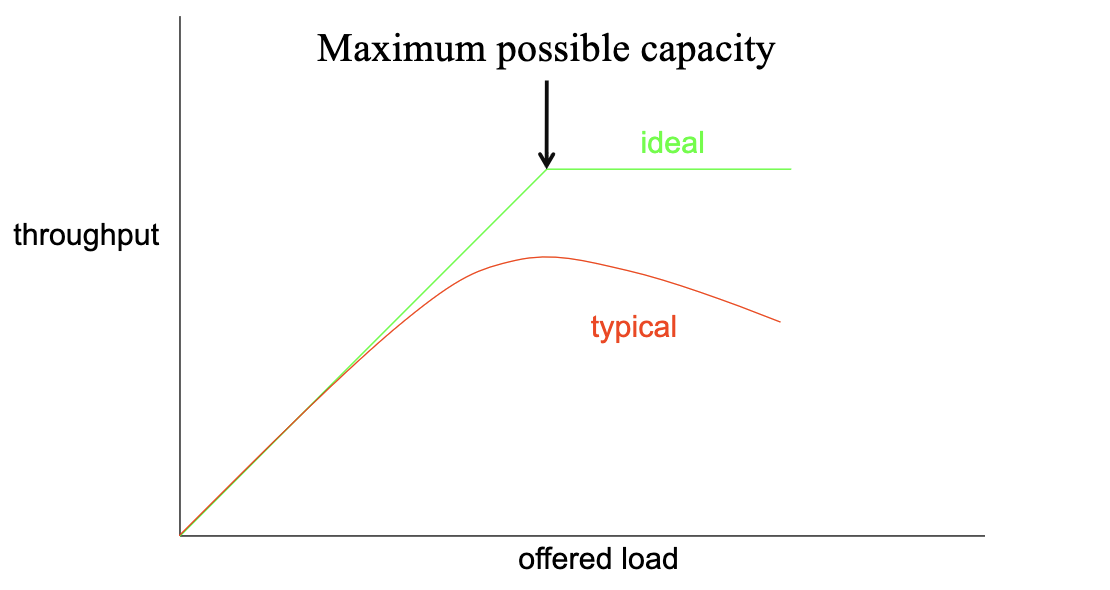
\includegraphics[scale=0.4]{images/throughput.png}
\end{center}

This happens because scheduling isn't free! It takes time to dispatch a process (overhead). More
dispatches mean more overhead (lost time). Consequently, less time (per second) is available to run
processes. Naturally, we can try minimizing the performance gap by reducing the overhead per dispatch and minimize the
number of dispatches.
\exampleEnd

\exampleBegin{Delay Doozy}
\begin{center}
  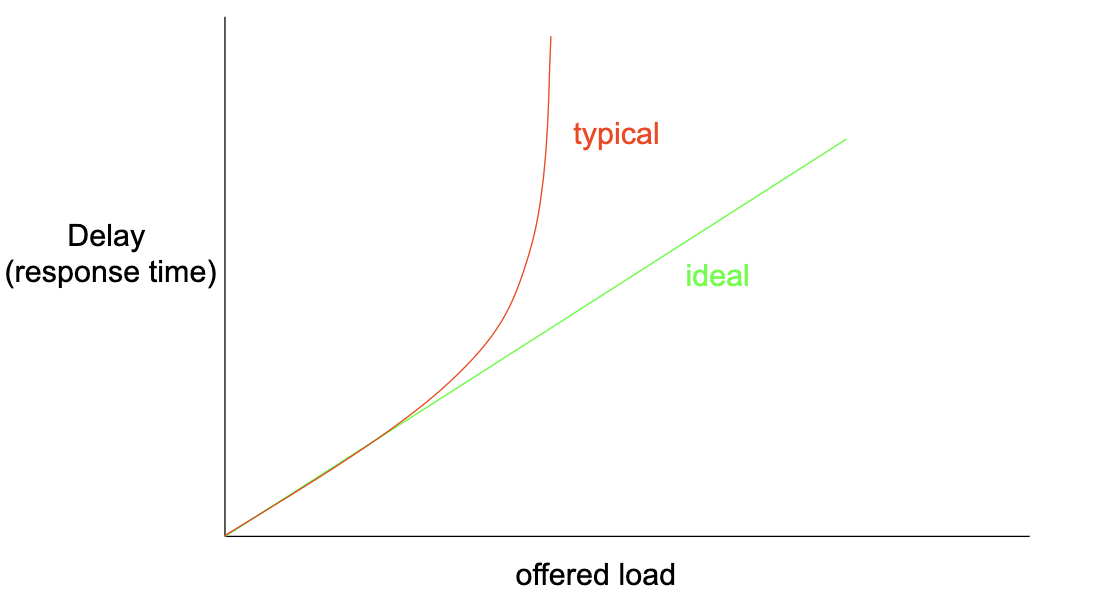
\includegraphics[scale=0.4]{images/delay.png}
\end{center}

This happens because real systems (unfortunately) have finite limits (like queue size). When limits
are exceeded, requests are typically \textit{dropped}\footnote{Dropped: We simply don't process the
  request}. From the requester's view, this looks like an infinite response time since the request
isn't begin serviced at all! Even if there are mechanisms like automatic retries (e.g. TCP
retransmissions), the retries themselves could also be dropped, further exacerbating the
situation. During these periods of heavy loads, the system performance drops severely since
overheads like context switching and memory management will explode. Careful system design and resource management can help to minimize this problem, but it is not
guaranteed to \textit{fix} the problem.
\exampleEnd


\subsection*{Graceful Degradation}
\addcontentsline{toc}{subsection}{Graceful Degradation}
\definitionBegin{Overload and Graceful Degradation}
A system is said to be \textbf{overloaded} when it can no longer meet its service goals.
\tcblower
\textbf{Graceful degradation} ensures that the system will continue service, but with degraded
performance.
\definitionEnd

When a system is overloaded, we want to use the graceful degradation principle to at least do
\textit{some} work. We \textit{never} want to allow throughput to drop to zero. This will allow
response times to grow without limit; i.e. this will lead to infinite response times!





\section{Non-Preemptive Algorithms}


\subsection{First Come First Serve}
The First Come First Serve (FCFS) algorithm consists of running the processes in the order that they
arrived. We run the first process on the ready queue until it completes or yields. One of the
primary characteristics of this algorithm is that it has highly variable delays since it relies on
the process order.

\bookBegin{FIFO/FCFS}
What happens when we relax assumption \textit{(i)} (See \textbf{\nameref{subsubsec:SM}})? Well,
long-running processes will monopolize CPU time, delaying the execution of shorter processes! This
results in poorer performance if a long-running process runs first.
\bookEnd

While FCFS ensures that all processes will eventually be served, it may not be the most efficient
since it can result in poor utilization of the CPU and inefficient response times. Long-running
processes will monopolize CPU time, delaying the execution of shorter processes.


\subsection{Shortest Job First}
The Shortest Job First (SJF) algorithm runs the processes in the order of their run-times. We run
the process with the shortest run-time on the ready queue until it completes or yields. One of the
primary characteristics of this algorithm is that it optimizes for throughput (good for batch
processing!).

\bookBegin{FIFO/FCFS}
What happens when we relax assumption \textit{(ii)} (See \textbf{\nameref{subsubsec:SM}})? Well, we
run into the same problem as FCFS if the long-running process arrives first! The long-running
process will monopolize CPU time, delaying the execution of the other processes! 
\bookEnd





\section{Real-Time Schedulers}
Real-time schedulers are used in systems with time-sensitive tasks. Deadlines can either be
\textit{hard}\footnote{Hard: Under no circumstances can the deadline be missed.} or
\textit{soft}\footnote{Soft: It isn't the end of the world if the deadline is missed.}.


\subsection{Hard}
Hard real-time schedulers rigorously enforce deadlines through careful analysis and pre-defined
schedules. Often times, this means that we know \textit{in advance} the schedule of processes to be
run. Therefore, there is no nondeterminism in your scheduler, and it is inherently non-preemptive.
These real-time schedulers are uncommon. 

\exampleBegin{Deadly Deadline}
Assume you have to write a scheduling algorithm to control a nuclear power plant. If you miss a
particular process deadline, your plant will probably blow up. So, you carefully analyze your
processes to come up with the \textit{perfect} schedule that will \textit{never} miss a
deadline. Since you know the processes in advance, there is no nondeterminism in your
schedule.
\exampleEnd


\subsection{Soft}
Soft real-time schedulers \textit{want} to meet deadlines, but it won't be the end of the world if
they don't. So, we want to optimize our scheduler to avoid missing deadlines. We can do so by giving
each process a priority level: the higher the priority, the sooner the deadline.

One possible algorithm is Earliest Deadline First (EDF), which will sort jobs based on deadlines,
minimizing total lateness.

If deadlines are missed, the system's response depends on its design and may involve dropping the
job, falling behind, or dropping future jobs to compensate.

\exampleBegin{Choppy Video}
When watching a video, the reason why it may be choppy at times is because the scheduler will drop
certain packets that missed their deadline! Thus, to the end user it appears choppy, probably
because their internet sucks (they might be using eduroam).
\exampleEnd





\section{Preemptive Algorithms}
\bookBegin{Preemptive Algorithms}
When we relax \textit{(iii)} (See \textbf{\nameref{subsubsec:SM}}), we get preemptive algorithms.
\bookEnd


\subsection*{Preface: Implementing Preemption}
\addcontentsline{toc}{subsection}{Preface: Implementing Preemption}
Preemption can be caused by syscalls or clock interrupts. Before returning control to the process,
the scheduler is consulted to determine if there are higher-priority ready processes or any
processes that need to be woken up. The scheduler will find the highest priority ready process,
switching to it (if it's not the current process), effectively preempting the current process.

We can use clock interrupts to do this. Modern CPU's have a clock peripheral device that can
generate interrupts at fixed time intervals. These clock interrupts will temporarily halt the
currently running process, transferring control to the scheduler, allowing for preemptive scheduling.


\subsection{Round Robin}
\label{subsubsec:RR}
The Round Robin (RR) algorithm consists of assigning a time slice to all processes (usually the same
size). Processes are scheduled as they arrive and run until they either block or their time slice
expires. After running, the process is put at the end of the process queue. Eventually each process
will get a turn to run for its allotted time slice.

Some key characteristics of RR is that this usually results in faster response times (for
interactive applications), but since more context switches occur, they can be
expensive. Additionally, runaway processes have less impact since they only take a fraction of the
overall cycles, and will not run forever.

\bookBegin{Round Robin}
Note that ``fair'' algorithms like RR will perform poorly in turnaround time. Thus, we use response
time to measure such algorithms. Now, relaxing assumption \textit{(iv)} (See
\textbf{\nameref{subsubsec:SM}}), we can see that there may be gaps where the CPU isn't doing
anything! To remedy this, we want to move the process to the back of the process queue whenever the
process halts, \textit{regardless} of how (I/O, interrupt, etc.). This way, the CPU is
\textit{always} doing something useful.
\bookEnd


\subsection{Choosing a Time Slice}
The duration of the time slice is crucial for optimizing performance. Longer time slices reduce the
frequency of context switches, but are bad for response times. Shorter time slices are better for
response time, but are more expensive since they require more context switches. Striking the right
balance is important!


\subsection{Cost of Context Switches}
When a context switch occurs, the OS goes through several steps, handling the interrupt, saving
register values, and invoking the scheduler, all of which incur overhead. Additionally, context
switching involves changing the stack and handling non-resident process descriptions. Furthermore,
the switch requires mapping out the old and new processes, affecting the efficiency of address space
changes. More notably, the loss of instruction and data caches significantly impacts the speed of
subsequent instructions, reducing overall performance.





\section{Priority Algorithms}
\definitionBegin{Starvation}
\textbf{Starvation} refers to when processes that have low priority don't run very often or don't
run at all.
\definitionEnd

Priority scheduling assigns each process a particular priority level (higher usually meaning more
important). Priority scheduling depends on if the scheduler is preemptive or
non-preemptive. Non-preemptive priority schedules simply dictate the order the processes will run
in. However, if the scheduler is preemptive, we may have a case where, when a new process is
created, it preempts the running process (assuming the new process has higher priority). One concern
for preemptive priority algorithms is the possibility of starvation.


\subsection{Hard and Soft}
\definitionBegin{Hard and Soft Priorities}
A \textbf{hard priority} refers to when processes with the highest priority has absolute precedence
over lower-priority processes and can preempt them to gain immediate access to the resource.
\tcblower
A \textbf{soft priority} refers to when resources are allocated according to their priority
level. Higher priority processes receive a larger share of resources, but lower-priority
processes aren't blocked entirely.
\definitionEnd

\exampleBegin{Linux Priorities}
Linux uses soft priorities, represented by a ``nice value'' assigned to each process. The nice value
indicates the share of CPU resources a process should receive. Users can adjust priorities using
specific commands, but can only request \textit{lower} priorities. Higher priorities can only be
requested by privileged users.
\exampleEnd


\subsection{Multi-Level Feedback Queue}
\bookBegin{Multi-Level Feedback Queue}
What happens when we relax assumption \textit{(iii)} (See \textbf{\nameref{subsubsec:SM}})? We get
the Multi-Level Feedback Queue! This scheduler is so important that there's an entire chapter
dedicated to it!
\bookEnd

The Multi-Level Feedback Queue (MLFQ) is a technique that uses multiple ready queues with varying
time slices to accommodate different types of processes. We want to optimize both response time for
interactive tasks and minimize overhead for longer background tasks. The foreground queue with
shorter time slices (high priority) is used for quick responses. The background queue with longer
time slices (low priority) minimizes overhead.

When a new process enters the scheduler, it is initially placed in the high priority queue. Once its
time slice expires, the process is then moved to the low priority queue. Periodically, all processes
are moved back to the high priority queue to prevent starvation!

MLFQ achieves acceptable response times for interactive jobs without wasting CPU
resources. Additionally, the scheduler dynamically adjusts based on the actual behavior of jobs,
providing an automatic and adaptive scheduler!










\chapter{Memory Management}
\label{chap:MM}
There are three primary goals for memory management:
\begin{enumerate}[label=\textit{(\roman*)}]
\item Transparency: Processes should only be able to see their own address space. That is, their
  address space is isolated, and processes are oblivious of any memory sharing with other
  processes. This ensures data privacy and security.
\item Efficiency: The system should utilize memory efficiently to optimize resource allocation and
  minimize waste. The allocation and (when necessary) relocation of memory should be performed with
  low run-time overhead to maximize system performance.
\item Protection and isolation: We want to ensure that the data within a process remains protected
  and is isolated from outside processes. That is, other processes can neither access it nor modify
  it.
\end{enumerate}
The memory management problem involves several key aspects:
\begin{enumerate}[label=\textit{(\roman*)}]
\item Unpredictability: Processes usually cannot accurately predict the exact amount of memory they
  will require during execution.
\item Continuity Expectations: Processes expect to find their existing data where they left it,
  implying that processes assume they have a contiguous address space.
\item Limited Physical Memory: The total memory required by all the processes may exceed the
  available physical memory.
\item Efficient Process Switching: We need to optimize the delay for copying data.
\item Low Overhead: The cost of memory management should be minimized to maximize system performance.
\end{enumerate}





\section*{Preface: Physical and Virtual Addresses}
\addcontentsline{toc}{section}{Preface: Physical and Virtual Addresses}
\definitionBegin{Physical and Virtual Memory Addresses}
\textbf{Physical memory addresses} refer to the actual hardware location of a particular memory
block.
\tcblower
\textbf{Virtual memory addresses} are an \textit{abstraction} over physical memory addresses, and
are \textit{not} the same as physical addresses. They represent a contiguous block of memory, when
in reality the physical addresses may be scattered.
\definitionEnd

Virtual memory addresses are used in processes and allow for more flexibility in memory management,
but require a virtual to physical translation unit. 





\section*{Preface: Fragmentation}
\addcontentsline{toc}{section}{Preface: Fragmentation}

\definitionBegin{Internal and External Fragmentation}
\textbf{Internal fragmentation} occurs when there is wasted space \textit{inside} a block of
allocated memory. That is, the requester was given more memory than he needed.
\tcblower
\textbf{External fragmentation} occurs when there is free space in the memory that cannot be used to
satisfy any memory allocation request since the available free memory is fragmented into smaller,
non-contiguous blocks. As a result, the total amount of free memory may satisfy the request, but
since the memory isn't contiguous, we cannot fulfill it.
\definitionEnd





\section{Fixed Partition Allocation}
Fixed Partition Allocation divides the available memory into fixed-size partitions (go figure), and
each partition is assigned to a specific process. The number of partitions is pre-allocated and is
based off the expected number of processes and their sizes. Each process can only access the
partition assigned to it and cannot access the memory allocated to other processes.

This approach is relatively easy to implement and was used in early batch processing systems. The
de/allocation of partitions are straightforward and efficient. However, it is not very flexible
since it requires a predetermined number of partitions and may lead to inefficient memory
utilization if the partition sizes are not well-matched with the actual memory requirements of the
processes.

To enforce memory protection, hardware support is often used. Special registers that hold the
partition boundaries ensure that each process can only access memory within its allocated
partition. However, fixed partition allocation does not use virtual addresses, meaning the processes
use the physical addresses directly.


\subsection{Problems}
\label{subsec:PROB}
There are several problems with Fixed Partition Allocation:
\begin{enumerate}[label=\textit{(\roman*)}]
\item Static Allocation: Fixed Partition Allocation requires knowing the exact memory requirements
  of all processes in advance, making it challenging to handle dynamic memory demands.
\item Limitations: The number of partitions defines the maximum number of processes that can be
  accommodated concurrently. If the partitions are not efficiently sized or the number of processes
  exceed the partition count, some processes may not be able to run concurrently.
\item Inefficient: Some partitions may be unused or underutilized, leading to poor memory
  utilization.
\item Limited Sharing: Processes cannot easily share memory, making it difficult to implement
  communication and data sharing between processes.
\item Internal Fragmentation: If partitions are not efficiently sized, they may succumb to internal
  fragmentation, leading to wasted memory.
\end{enumerate}
Because of these reasons, this approach isn't commonly used in modern operating systems.





\section{Dynamic Partition Allocation}
Dynamic Partition Allocation allows variable-sized partitions which accommodate almost any size
requested. Each partition has contiguous addresses, and processes are allowed to access the
partitions it requested. These partitions can be shared between multiple processes, and a single
process may have multiple partitions with different sizes and characteristics. However, in the basic
scheme, memory addresses are still physical, which can lead to external fragmentation and limited
address space. 


\subsection{Problems}
\label{subsec:PROB2}
There are several problems with Dynamic Partition Allocation:
\begin{enumerate}[label=\textit{(\roman*)}]
\item Not Relocatable: Once a partition is allocated, it is very hard to relocate its contents to
  another memory location, which can lead to inefficient memory utilization.
\item Not Expandable: Dynamic partitions are limited in their ability to grow/shrink to
  accommodate changing memory requirements of processes.
\item Limited Support: Dynamic partitions may struggle to support address spaces larger than
  physical memory, hindering their ability to handle memory-intensive jobs.
\item External Fragmentation: As processes de/allocate memory over time, dynamic partitions can
  suffer from external fragmentation, leading to wasted memory.
\end{enumerate}
Relocation and expansion can be challenging in dynamic partition allocation because partitions
are tied to specific address ranges during execution. Relocating the contents of a partition require
updating all the pointers within the contents, which is not always feasible, especially if you don't
know which memory locations contain pointers. Additionally, expanding a partition may be challenging
since there may not be enough contiguous free space. These limit the usefulness of dynamic partition
allocation. 





\subsection{Managing Variable-Sized Partitions}
\label{subsec:FL}
\definitionBegin{Free List}
The \textbf{free list} is a data structure (often implmented with a list or array) that keeps track
of all available chunks of unallocated memory.
\definitionEnd

To manage variable-sized partitions, the memory manager starts with a single large block of memory
known as the ``heap'', and maintains a data structure called the ``free list''. When a process
requests memory, the memory manager will consult the free list, carving a chunk (of the requested
size) and putting the remainder back onto the free list. When processes deallocate memory, it is put
back onto the free list.





\section{Free-Space Management}
Fixed sized blocks are easy to track: we can use a bitmap to indicate which blocks are free.

Variable chunks require more information. Each chunk of memory has a descriptor containing
information about its free status, chunk size, and a pointer to the next chunk. These chunks are
typically organized into a linked list.

Variable sized partitions are not as subject to internal fragmentation since processes, in theory,
request the exact amount of memory needed. However, they are subject to external fragmentation. We
can minimize external fragmentation by consulting an algorithm to determine how we manage our free
list.


\subsection{Best Fit}
The best fit algorithm will search for the \textit{smallest} available chunk that meets the size
requirements. This minimizes memory waste and reduces internal fragmentation.

\begin{tcbraster}[raster columns=2, raster equal height, raster force size=false]
  \begin{tcolorbox}[colback=green!5!white,colframe=black!75!green,title=Advantages]
    \begin{enumerate}[label=\textit{(\roman*)}]
    \item Increased odds of a (near) perfect fit.
    \end{enumerate}
  \end{tcolorbox}
  \begin{tcolorbox}[colback=red!5!white,colframe=black!40!red,title=Disadvantages]
    \begin{enumerate}[label=\textit{(\roman*)}]
    \item An exhaustive search is necessary.
    \item Quickly creates small fragments.
    \end{enumerate}
  \end{tcolorbox}
\end{tcbraster}


\subsection{Worst Fit}
The worst fit algorithm will search for the \textit{largest} available chunk that meets the size
requirements. This tries to minimize memory waste by creating large fragments.

\begin{tcbraster}[raster columns=2, raster equal height, raster force size=false]
  \begin{tcolorbox}[colback=green!5!white,colframe=black!75!green,title=Advantages]
    \begin{enumerate}[label=\textit{(\roman*)}]
    \item Tends to create large fragments.
    \end{enumerate}
  \end{tcolorbox}
  \begin{tcolorbox}[colback=red!5!white,colframe=black!40!red,title=Disadvantages]
    \begin{enumerate}[label=\textit{(\roman*)}]
    \item An exhaustive search is necessary.
    \item Over time, small fragments are inevitable.
    \end{enumerate}
  \end{tcolorbox}
\end{tcbraster}


\subsection{First Fit}
The first fit algorithm will search for the \textit{first} available chunk that meets the size
requirements. This reduces overhead since there's no need (potentially) to search exhaustively.

\begin{tcbraster}[raster columns=2, raster equal height, raster force size=false]
  \begin{tcolorbox}[colback=green!5!white,colframe=black!75!green,title=Advantages]
    \begin{enumerate}[label=\textit{(\roman*)}]
    \item Creates random sized fragments.
    \item Doesn't require an exhaustive search.
    \end{enumerate}
  \end{tcolorbox}
  \begin{tcolorbox}[colback=red!5!white,colframe=black!40!red,title=Disadvantages]
    \begin{enumerate}[label=\textit{(\roman*)}]
    \item The first chunks quickly fragment
    \item Over time, the searches become longer.
    \end{enumerate}
  \end{tcolorbox}
\end{tcbraster}


\subsection{Next Fit}
The next fit algorithm will search for the \textit{first} available chunk that meets the size
requirements \textit{starting from the last allocation point} instead of the beginning of the free
list. This reduces overhead and tries to minimize fragmentation.

\begin{tcbraster}[raster columns=2, raster equal height, raster force size=false]
  \begin{tcolorbox}[colback=green!5!white,colframe=black!75!green,title=Advantages]
    \begin{enumerate}[label=\textit{(\roman*)}]
    \item Creates random sized fragments.
    \item Reduces overhead since we don't start from the beginning.
    \end{enumerate}
  \end{tcolorbox}
  \begin{tcolorbox}[colback=red!5!white,colframe=black!40!red,title=Disadvantages]
    \begin{enumerate}[label=\textit{(\roman*)}]
    \item Over time, memory chunks still fragment.
    \item Over time, the searches become longer.
    \end{enumerate}
  \end{tcolorbox}
\end{tcbraster}





\section{Coalescing Partitions}
Coalescing partitions is a technique used to reduce external fragmentation in variable-sized
partition allocation algorithms. When a process frees a chunk of memory, the memory management
system checks if the neighboring chunks are also free. If they are, the system combines them into a
larger, contiguous block, reducing fragmentation.

\bookBegin{Free-Space Management}
To simplify the coalescing process, we can organize the free list such that neighboring chunks are
placed close to each other. One way to do this is by ordering the free list by addresses, making it
more efficient to find neighboring chunks and merge them when necessary.
\bookEnd

Coalescing helps minimize external fragmentation by reducing the number of small, unusable gaps
between allocated memory blocks. However, it is worth noting that it doesn't \textit{completely}
eliminate external fragmentation since it can only merge \textit{contiguous} chunks.

When multiple processes operate in parallel, it's challenging to predict which process will dominate
and how they will interact, leading to potential fragmentation issues. The fraction of space
typically allocated depends on the number and size of processes running; if a significant portion of
memory is allocated, coalescing becomes less effective due to limited free space.

Additionally, the speed of allocated memory turnover affects coalescing; processes holding memory
chunks for extended periods reduce the effectiveness of coalescing. Note that coalescing only
minimizes fragmentation since external fragmentation will \textit{always} occur over time.





\section{Buffer Pools}
Certain chunk sizes are requested more frequently than others. Key services like I/O, network
protocols, etc. usually work with fixed-size buffers. Thus, we can reserve special pools of
fixed-size buffers for popular buffer sizes.

\definitionBegin{Buffer Pool}
A \textbf{buffer pool} is a reserved section of fixed-sized memory buffers used to handle frequently
requested memory sizes (like Reiher's favorite 4K), reducing memory management overhead and external
fragmentation.
\definitionEnd

Buffer pools are used to handle frequently requested memory sizes efficiently. When there are
popular buffer sizes, the operating system can reserve special pools of fixed-size
buffers. When a request for a matching buffer size arrives, it is taken out of the buffer pool as
opposed to the free list. This reduces external fragmentation and memory management overhead.

However, the OS needs to determine an appropriate size for the buffer pool. Too small and it might
not improve efficiency. Too large and it might lead to a lot of unused buffer space.
It is also worth noting that buffer pools will only satisfy \textit{perfectly} matching requests,
since otherwise we get internal fragmentation.


\subsection{Sizing}
We dynamically adjust the size of the buffer pool based on the system load and buffer
availability. When the pool runs low on fixed-size buffers, we simply acquire more memory from the
free list\footnote{If the free list gets dangerously low, we ask each major service with a buffer
  pool to return space.} and divide it into new buffers. When the pool is too large, we release some
buffers back into the free list. We can tune these thresholds (low space and high space) to
determine when to adjust the buffer pool size. This approach makes the system highly adaptive to
changing workloads and memory requirements.





\section{Memory Leaks}
\definitionBegin{Memory Leak}
A \textbf{memory leak} is when memory is allocated but never freed, causing the memory to remain
occupied indefinitely.
\definitionEnd

Memory leaks in the context of buffer pools occur when a process is done with a buffer, but fails to
free it. This causes the buffer to remain in the pool indefinitely, wasting memory. Long running
processes with memory leaks can result in substantial memory waste over time. Addressing memory
leaks is crucial if we want efficient memory utilization.

\exampleBegin{Leaky Program}
Assume you have a small program that allocates some memory and immediately terminates. You are
surprised that there are no memory leaks! However, this is just because when a process dies,
\textit{all} of its memory gets reclaimed, \textit{implicitly} freeing the memory you allocated in
your program. But what if you had a \texttt{while (true)} loop in your code? Since you aren't doing
anything with that memory, it's probably a good idea to let someone else use it! But, since you
never explicitly freed it, the memory you allocated is inaccessible (until the process terminates)!
Because of this, It is generally bad practice to not \textit{explicitly} free any memory you
\textit{explicitly} allocate. 
\exampleEnd





\section{Garbage Collection}
Garbage collection (GC) is a technique to address memory leaks and reclaim unused memory. Instead of
relying on processes to release memory on their own, garbage collection monitors the amount of free
memory left on the system. When there is \textit{memory pressure}\footnote{Memory pressure: When the
  amount of free memory becomes dangerously low.}, garbage collection is triggered.

The system will search the data space to identify all reachable objects, noting their address and
size. Then, any unreachable objects (inaccessible memory) is then reclaimed and added back into the
free list. This ensures that memory is efficiently utilized and helps prevent memory leaks!


\subsection{Determining Accessible Memory}
In general, we want to identify and reclaim memory that is no longer used. To do this, we do the
following:

\begin{enumerate}[label=\textit{(\roman*)}]
\item Find all pointers in allocated memory: We need to traverse \textit{all} allocated memory to
  locate the pointers that reference other objects/data.
\item Determine the size of each pointer: We must determine the size and extent of the memory
  region each pointer references.
\item Determine what is/n't pointed to: We need to identify objects that are still accessible and in
  use by actively referenced pointers.
\item Free inaccessible memory: We put all inaccessible memory back into the free list.
\end{enumerate}
GC can be difficult because it requires comprehensive scanning of the entire memory space to
identify references and determine object boundaries. Furthermore, it also needs to be able to handle
complex references (e.g. cyclic data structures) for accurate identification of unused
memory. Additionally, GC takes time, and therefore can slow down system performance.


\subsection{Problems}
There are several problems we need to address:
\begin{enumerate}[label=\textit{(\roman*)}]
\item Identifying pointers are \textit{hard}. Locations in a program's data or stack segments may
  \textit{appear} to contain addresses but are actually just data (that \textit{resembles}
  addresses). We need to accurately identify valid pointers to avoid reclaiming active memory.
\item Even if pointers are identified, we need to determine if they are still accessible and in use! This
  requires recursive analysis of dynamically allocated data structures to ensure that all referenced
  memory remains reachable. Even so, statically allocated data structures are harder to analyze.
\item We also need to determine the size of each object pointed to, which can be challenging! Measuring
  exact boundaries may be hard for complex data structures or objects with variables sizes.
\end{enumerate}





\section{Memory Compaction and Relocation}
GC is simply another method to release memory, and therefore doesn't significantly impact
fragmentation. Ongoing memory de/allocations can prevent coalescing, leading to fragmentation over
time\footnote{Frequent allocations can starve coalescing, reducing its effectiveness.}. 

To counter this, we can compact active memory to one end, coalescing the other end to eliminate
fragmentation! However, this requires relocation, which is extremely complicated, since we need to
update all memory references correctly.

When a process is relocated, all addresses within the program will become invalid, resulting in
potential errors and crashes. We would need to:

\begin{enumerate}[label=\textit{(\roman*)}]
\item Update all references in the code segment (e.g. calls and branches to other parts of code) to
  point to the correct memory addresses in the new location.
\item Update referees to variables in the data segment to point to the correct addresses in the new
  location.
\item Ensure that new pointers are adjusted to point to the correct addresses after relocation.
\end{enumerate}
To solve the relocation problem, we can make the process location independent! By doing this, we can
avoid the complexities of update memory references, \textit{abstracting} away \textit{(i) -- (iii)}! We want to enable processes to execute in \textit{any} part of memory
without adjusting memory addresses. 

We can achieve this using various techniques:
\begin{enumerate}[label=\textit{(\roman*)}]
\item Relative addressing: We can use offsets instead of absolute memory addresses to allow
  processes to be loaded into different memory locations with no address modifications.
\item Base and Bounds Registers: We can use hardware registers (base and bound registers) to
  automatically adjust memory references at runtime. These registers keep track of the base address
  and size (bound) of the process' memory space, allowing the CPU to translate relative addresses
  into absolute addresses during execution.
\item Virtual Memory and Paging: We can use VM techniques like paging to abstract the physical
  memory from the process' address space. This way, the process can work with the virtual addresses
  that get translated to physical addresses, making the process independent of its location.
\end{enumerate}

\abstractionBegin{Virtual Memory}
Virtual memory is an \textit{abstraction} over physical memory! A virtual address is \textit{not}
the same as its corresponding physical address, and requires a translation unit to convert between
the two. However, this is a small price to pay for making memory relocation \textit{significantly}
easier!
\abstractionEnd


\subsection{Segment Relocation}
Memory segment relocation is a technique that involves organizing a process' address space into
multiple segments, each representing a contiguous block of memory with a specific purpose (see
\refto{subsec}{PAS}). The segments are then moved as a unit during relocation.


\subsection{Base and Bounds Registers}
Computer architecture may include special relocation registers known as segment \textit{base
  registers}. These registers hold the starting address of each segment in physical memory. When the
CPU accesses a memory location, it will add the address to the address of the base register,
translating the virtual address to the physical address!

When a program is loaded into memory, the OS sets the base registers to the start of the
program. When relocating, we simply update the base register accordingly. This way, the program can
continue to run smoothly regardless of where it is located in physical memory.

\corollaryBegin{Security}
We still need to protect our memory! Protection refers to preventing a process from accessing memory
outside its allocated memory. To achieve this, we utilize a length (or limit) register, often
called the \textit{bounds register}, which specifies the maximum valid offset from the start of the
segment. Any address greater than the limit is considered illegal and should be inaccessible to the
process. \\

When processes attempt to access an illegal address, the CPU triggers a segmentation exception or
trap. This exception traps into the OS allowing it to take appropriate action (e.g. terminating the
process or controlling the violation).
\corollaryEnd





\section{Swapping}
Swapping is a technique to overcome the limitation of physical RAM by temporarily storing inactive
processes' memory on disk. When a process isn't actively running (e.g. yields, blocked), its entire
memory contents are copied to disk to free up RAM for other processes.

When a process is scheduled to run again, its memory is then copied back from disk onto RAM to
continue execution. If the system has relocation hardware, the memory can be placed in different RAM
locations, enabling processes to access their memory regardless of their physical addresses. This
allows the system to use disk space as a virtual extension of physical memory, giving the 
\textit{illusion} that each process gets all of RAM to itself. 

However, swapping incurs overhead since copying is expensive! The cost of a context switch are
\textit{very} high, since we need to:

\begin{enumerate}[label=\textit{(\roman*)}]
\item Copy all of RAM out to disk.
\item Copy other stuff from disk to RAM.
\end{enumerate}
\textit{before} the new process can do anything. Moreover, we still cannot exceed the amount of
physical RAM, which can limit memory-intensive processes or overall system performance.





\section{Paging}
\label{sect:PGING}
Paging is a technique that divides both physical memory and virtual address space into fixed-size
units\footnote{Usually 1-4K bytes or words.} called \textit{pages}. The pages in physical memory are
referred to as \textit{page frames}, while pages in virtual memory are just called \textit{pages}.

Each virtual page is mapped to a physical page frame, but it's not fixed nor is it
one-to-one. Instead, a per-page translation mechanism called a \textit{memory management unit
  (MMU)}\footnote{The Memory Management Unit (MMU) is hardware (often integrated into the CPU)
  responsible for handling memory access and virtual-to-physical address translation.},
is used to dynamically translate virtual page numbers to corresponding physical page frame
numbers. 


\subsection{Big Page Tables}
\definitionBegin{Translation Lookaside Buffer}
The \textbf{Translation Lookaside Buffer (TLB)} is the MMU cache that stores a subset of recently
accessed page table entries. This improves lookup times since we don't have to access page table
entries from main memory for \textit{every} memory access.
\definitionEnd

Traditionally, page tables were implementing using fast registers in the MMU. But with larger memory
sizes and smaller page sizes, there will be a \textit{lot} of pages.

\exampleBegin{How Many Pages?}
Suppose you have 64 GB memory with 4K page sizes. There would be $\frac{64 \textit{GB}}{16
  \textit{KB}} = 16$ \textit{million} pages! Unfortunately, we cannot afford to store 16 million
pages into fast registers. 
\exampleEnd

\definitionBegin{TLB Hit and Miss}
A \textbf{TLB hit} is when the required translation is found in the TLB.
\tcblower
A \textbf{TLB miss} is when the required translation is \textit{not} in the TLB, and an access to
the page table is necessary.
\definitionEnd
To remedy this, TLB's act as a high-speed cache for virtual-to-physical address translations,
reducing overhead. When the CPU needs to translate a virtual address, it first checks the TLB. If
the translation is found in the TLB, we return it. Otherwise, we need to consult the page table in
main memory to retrieve the required page table entry. The TLB is then updated accordingly.

Unfortunately, the TLB has a limited size, and therefore not all entries can fit into it. This lead
to the issue of cache invalidation and replacing entries when the TLB is full. Maintaining a high
TLB hit ratio is crucial for efficient VM performance.


\subsection{Swap Space}
\definitionBegin{Page Fault}
A \textbf{page fault} is when the required address is not in the TLB, is valid, but is not present
(i.e. it is in the swap space or page file). 
\definitionEnd

Since we have more pages than RAM, we need to store some of them somewhere other than
RAM. Typically, some pages are kept on disk and are referred to as the \textit{swap space} or
\textit{page file}. When a page fault occurs, the OS retrieves\footnote{In the meantime, other
  processes can execute} the required page from the swap space, loading it into an available page
frame in RAM. The program counter is backed up to retry the failed instruction after the page is
loaded, allowing the process to continue running.  


\subsection{Ongoing Operations}
The MMU has many ongoing operations. Here are three important ones:
\begin{enumerate}[label=\textit{(\roman*)}]
\item Adding/Removing Pages: When the current process dynamically de/allocates memory, the MMU
  needs to reflect this in the page table. The OS will directly update the active page table in
  memory to adjust the relevant page mappings. A privileged instruction is used to flush any stale
  cached entries in the MMU to ensure an accurate mapping.
\item Context Switching: When the system switches processes, the MMU needs to switch the appropriate
  page table for the new process. Each process has a separate page table, and a privileged
  instruction is used to load the pointer to the new page table. Before the new process begins
  execution, a reload instruction flushes any previously cached entries, preventing invalid access.
\item Page Sharing: Page sharing allows for memory sharing between multiple processes. The page
  tables can be configured to point to the same \textit{physical} page. This means multiple
  processes can have access to the same page in RAM. Page sharing can be read/write or read-only
  depending on access requirements and memory protection mechanisms enforced by the OS. This
  approach is good for sharing read-only data (e.g. code segments, shared libraries), reducing
  redundancy.
\end{enumerate}


\subsection{Demand Paging}
Demand paging is a technique where not all pages of a process are loaded into RAM at once. Rather,
only pages that are actively being referenced are brought into memory when needed, allowing for
better memory efficiency and less overhead during process scheduling and context switching.

Demand paging frees up RAM by keeping the majority of a process' data on disk until it's actually
needed, enabling the system to accommodate more processes and improves overall memory
utilization. Demand paging utilizes page faults to signal when pages need to be fetched from disk. 

One problem of demand paging is performance optimization. Frequent page faults incur overhead since
the time it takes to fetch from disk can add up. Efficient page replacement algorithms like
\textit{Least Recently Used (LRU)}\footnote{The page that hasn't been accessed for the longest
  period of time is booted from RAM.} are used to minimize the number of page faults triggered to
ensure that relevant pages are kept in RAM.


\subsection{Locality of Reference}
\label{subsec:LOR}
Locality of reference suggests that the next address a program will access is most likely to be
close to the one it just accessed. This is usually present in programs since they often execute
sequences of consecutive (or nearby) instructions, have short branches, access data in the
current/previous stack frame, and (tend to) access recently allocated heap structures. While there
are no guarantees, identifying these trends help reduce the number of page faults.










\chapter{Virtual Memory}
Virtual memory (VM) is a generalization of demand paging, and is a technique that provides a large
and uniform address space to each process. It gives the \textit{illusion} that each process has
access to a vast amount of memory (much larger than the physical RAM available).

\abstractionBegin{Virtual Memory and Paging}
Virtual memory is an \textit{abstraction} over demand paging. It extends the concept of paging by
providing a much larger address space to each process by using dynamic paging and swapping.
\abstractionEnd

Processes can directly request segments in this space, and the virtual memory system handles the
mapping of virtual to physical addresses via page tables. VM allows processes to run even if their
entire address space doesn't fit into physical memory. Instead, only actively referenced portions
are loaded into RAM, while the rest sits on disk.





\section{Replacement Algorithms}
Replacement algorithms are the key technology to making virtual memory work. We want to have the
relevant pages loaded into RAM when a process needs to access them.

We do this by relying on the principle of locality of reference. Doing this allows us to make smart
choices about which pages to keep in memory and which ones to kick to disk.

Page replacement happens when we need to free up space in memory for new pages. Whenever a page
fault occurs, we select an appropriate page to replace via an algorithm (like LRU).


\subsection{The Optimal Algorithm (Belady's Algorithm)}
The optimal replacement algorithm replaces the page that will be accessed furthest into the future,
minimizing the number of page faults. However, this requires an oracle, and as such, it is
impossible to implement. This algorithm is also known as ``Belady's Algorithm''.


\subsection{FIFO and Random}
According to Reiher (and common sense), these are dogshit so I'm not going to cover them.


\subsection{Least Frequently Used}
The Least Frequently Used (LFU) policy kicks the least frequently used page back to disk. It isn't
the best in the world.


\subsection{Least Recently Used and Clock Algorithm}
\label{subsec:LRU}
Least Recently Used (LRU) policy kicks the page with the oldest timestamp back to disk. This is done
(naïvely) by timestamping each time a page is accessed. When a page needs to be replaced, we search
through all pages to kick the one with the oldest timestamp. This incurs a lot of overhead and
therefore is not commonly used.

Rather, we usually use an approximate LRU, or ``Clock Algorithm''. We maintain a circular buffer of
pages in memory, with each page having an additional reference/use bit (typically stored in the
MMU). When a page is accessed, we set the reference bit to 1, indicating it has been recently
used. When determining the page to replace, we scan starting at a fixed point, replacing the first
page with reference bit 0.

This algorithm, while not a perfect one-to-one with LRU, offers performance on par with LRU for a
fraction of the cost. Therefore, it is usually implemented in favor of a ``true'' LRU.





\section{Page Replacement}
We don't want to clear out \textit{all} page frames on each context switch as it can be
inefficient. There are several ways to deal with this:

\begin{enumerate}[label=\textit{(\roman*)}]
\item Single Global Pool: All processes share a single pool of page frames in memory. When a process
  runs, it uses any available free page frame for its page.
\item Fixed Allocation per Process: Each process is assigned a fixed number of page frames when it
  starts. The number of page frames stays constant throughout execution.
\item Working Set-Based Allocations: The working set of a process represents the set of pages it is
  actively referencing at any given time. Page frames are allocated dynamically based on a process'
  working set. When a process runs, its working set is loaded into RAM, and when it's switch out,
  its page frames are potentially freed.
\end{enumerate}


\subsection{Single Global Pool}
In the Single Global Pool approach, all page frames in memory are treated as a shared resource, and
an approximation of LRU is used as the replacement algorithm. However, this sucks when paired with
round-robin scheduling (see \refto{subsubsec}{RR}).

\exampleBegin{Fair or Unfair}
In RR scheduling, the process that was last in the queue will find all of its pages swapped
out. Thus, when this process runs, it will experience a high volume of page faults since all of its
pages were replaced.
\exampleEnd

This is because this approach doesn't account for the specific working sets of each process. For
this reason, this approach is usually pretty dogshit.


\subsection{Per-Process Pools}
In the Per-Process Pool approach, a fixed number of pages are allocated for each process, and the
approximate LRU is used \textit{separately} for each process. This allows for dynamic and customized
allocation of page frames to each process.

However, a fixed number of pages per process sucks because different processes exhibit varying
levels of locality, and the pages needed by each process usually change over time. Moreover,
processes have different natural scheduling intervals, and as such, their memory requirements vary
throughout execution!


\subsection{Working Sets}
\definitionBegin{Working Set}
A \textbf{working set} is defined to be the set of pages a process actively referenced within a
fixed sampling interval in the immediate past.
\definitionEnd

Working sets are used to allocate page frames to each running process based on its specific memory
needs. We allocate a sufficient number of page frames to hold each process' working set. This
ensures that the frequency of accessed pages are kept in memory, reducing the volume of page
faults. Each process will manage its own set of pages, usually using an approximate LRU for page
replacement. 

Working sets dynamically adjust the allocation of page frames for each process based on its current
behavior, optimizing memory usage and responding to changes in workload and access patterns.


\subsection*{Optimal Working Sets}
The optimal working set for a process is the set of pages it needs during its next time slice (or a
specific period of time). Allocating less than the optimal amount leads to a lot of page faults.

We determine the size of the working set by observing the process' behavior over time. Tracking the
frequency of page faults and memory references, the system can identify which pages the process
frequently accesses, including them in the working set.


\subsection*{Page Stealing: Working Set-Clock Algorithm}
The Working Set-Clock algorithm tracks the last use time for each page for its owning process,
replacing the page that was least recently used.





\section{Thrashing}
\definitionBegin{Thrashing}
\textbf{Thrashing} refers to when a system spends a significant amount of time/resources swapping
pages between RAM and disk, but isn't able to efficiently make any progress in the executing
process.
\definitionEnd

Thrashing occurs when the total demand for memory by \textit{all} running processes exceeds the
available physical memory. When thrashing happens, we seldom execute any useful instructions since
so much time is spent swapping pages. This results in an underutilized CPU and degraded performance.

Thrashing typically happens hen the working set of each process exceeds the available physical
memory. When there are not enough page frames to accommodate the working sets of all active
processes, they constantly compete for memory.

To protect against thrashing, the OS takes proactive measures like reducing the degree of
multiprogramming (i.e. limiting the number of active processes), using page replacement algorithms
that prioritize larger working sets, or allocating more physical memory (lol). The goal is to avoid
thrashing by ensuring that each process has enough pages in memory to execute efficiently.

\exampleBegin{Everyone Gets a Turn}
When reducing multiprogramming, we can use a RR approach for swapping processes in and out of disk,
ensuring that all processes get a fair share of CPU time while minimizing thrashing!
\exampleEnd





\section{Clean and Dirty Pages}
\definitionBegin{Clean and Dirty Pages}
A \textbf{clean page} refers to a page in memory that hasn't been modified since it was brought from
disk. They can be safely replaced without needed to write them back to disk since their contents
match that of the one on disk.
\tcblower
A \textbf{dirty page} refers to a page in memory that has been modified or updated after it was
brought from disk. That is, the in-memory version of the page is different from the one on disk. If
a dirty page needs to be removed from memory, the page must be written back to disk to update the
appropriate page on disk, ensuring that the most recent version of the data is saved before kicking
it from memory. 
\definitionEnd

When given a choice, the OS will prioritize kicking clean pages since they can be safely removed
without the need for I/O. Dirty pages however, need to be written back to disk to preserve data integrity.





\section{Preemptive Page Laundering}
Preemptive page laundering is a technique used to increase the flexibility of the memory manager by
converting dirty pages to clean ones. Rather than waiting to write when pages gets kicked, we
initiate a background write-out of dirty pages that are not actively in use. This way, we reduce
the risk of thrashing and increase the number of clean pages we have.










\part{Concurrency}
\label{part:C}
\chapter{Threads}
\definitionBegin{Thread}
A \textbf{thread} is a unit of execution and scheduling in a program. Each thread has its own stack,
program counter, and registers, allowing it to operate independently of other threads.
\definitionEnd

Threads within the same process share the same code and data segment, making them more efficient and
less resource-intensive than processes.

In multi-threaded programs, multiple threads can run concurrently within the same process. They
share the process' resources (e.g. memory, files), but each thread maintains its own execution
state. This allows for better communication and coordination between different parts of the
program.

They can be implemented and managed in various ways. User-level threads are managed by the process
itself and rely on voluntary yielding. Scheduled system threads are managed by the OS and can be
preemptively scheduled, meaning the OS can interrupt it to give other threads CPU time.





\corollaryBegin{Why Not Processes?}
Processes are expensive! Since each one has private resources and a private address space, it makes
interprocess communication difficult. Additionally, certain programs may not require such strong
separation. So, we can use threads to remedy such limitations of processes.
\corollaryEnd





\section{Process v. Thread}
When should you use a process? A thread?

\begin{tcbraster}[raster columns=2, raster equal height, raster force size=false]
  \begin{tcolorbox}[colback=teal!5!white,colframe=black!75!teal,title=Processes]
    \begin{enumerate}[label=\textit{(\roman*)}]
    \item Running multiple, \textit{distinct} programs.
    \item Creation/destruction are \textit{rare} events.
    \item Running with distinct privileges.
    \item Limited interactions/shared resources.
    \item Strong separation between other processes.
    \end{enumerate}
  \end{tcolorbox}
  \begin{tcolorbox}[colback=yellow!5!white,colframe=black!75!yellow,title=Threads]
    \begin{enumerate}[label=\textit{(\roman*)}]
    \item Parallel activities in a \textit{single} program.
    \item Creation/destruction are \textit{frequent}.
    \item All can run with the same privilege.
    \item Need to shared resources.
    \item Frequent message/signal exchange.
    \item When you don't need protection from each other.
    \end{enumerate}
  \end{tcolorbox}
\end{tcbraster}


\subsection{Tradeoffs}


\subsubsection*{Processes}
\begin{tcbraster}[raster columns=2, raster equal height, raster force size=false]
  \begin{tcolorbox}[colback=green!5!white,colframe=black!75!green,title=Advantages]
    \begin{enumerate}[label=\textit{(\roman*)}]
    \item String isolation: Processes have distinct address spaces.
    \item Fault tolerance: Processes don't affect other processes.
    \item Easier resource cleanup: When a process terminates, all resources are automatically freed.
    \end{enumerate}
  \end{tcolorbox}
  \begin{tcolorbox}[colback=red!5!white,colframe=black!40!red,title=Disadvantages]
    \begin{enumerate}[label=\textit{(\roman*)}]
    \item Slower communication: Interprocess communication is more complex and slower.
    \item Potential duplication: Since each process has a distinct address space, this allows for
      unnecessary duplication.
    \end{enumerate}
  \end{tcolorbox}
\end{tcbraster}


\subsubsection*{Threads}
\begin{tcbraster}[raster columns=2, raster equal height, raster force size=false]
  \begin{tcolorbox}[colback=green!5!white,colframe=black!75!green,title=Advantages]
    \begin{enumerate}[label=\textit{(\roman*)}]
    \item Efficient communication: Threads share resources making communication and data sharing
      much faster.
    \item Lightweight: Threads have lower overhead since they share resources.
    \item Faster context switching: Switching between threads is faster than switching between
      processes because of \textit{(i)} and \textit{(ii)}.
    \end{enumerate}
  \end{tcolorbox}
  \begin{tcolorbox}[colback=red!5!white,colframe=black!40!red,title=Disadvantages]
    \begin{enumerate}[label=\textit{(\roman*)}]
    \item Synchronization issues: Threads must be synchronized to run properly.
    \item Increased complexity: Multi-threaded code is hard.
    \end{enumerate}
  \end{tcolorbox}
\end{tcbraster}





\section{Thread Stacks and State}
Each thread has its own stack, registers, program counter, and process status. The maximum stack size for
each thread is specified at creation, and needs to be managed carefully to avoid stack overflow or
memory waste. Since a process can contain many threads, they cannot all grow towards a single
hole. Thus, the thread creator needs to know the maximum required stack size. Moreover, stack space
must be reclaimed whenever threads exit.





\section{User v. Kernel Threads}
\begin{tcbraster}[raster columns=2, raster equal height, raster force size=false]
  \begin{tcolorbox}[colback=teal!5!white,colframe=black!75!teal,title=Kernel]
    \begin{enumerate}[label=\textit{(\roman*)}]
    \item Provided and managed by the OS kernel.
    \item Share the same address space.
    \item Scheduled by the kernel.
    \end{enumerate}
  \end{tcolorbox}
  \begin{tcolorbox}[colback=yellow!5!white,colframe=black!75!yellow,title=User]
    \begin{enumerate}[label=\textit{(\roman*)}]
    \item Managed by the user with no intervention from the OS kernel.
    \item Invisible to the kernel.
    \item Scheduled by the user.
    \end{enumerate}
  \end{tcolorbox}
\end{tcbraster}










\chapter{Interprocess Communication}
\definitionBegin{Interprocess Communication}
\textbf{Interprocess communication (IPC)} refers to the techniques provided by the OS to enable
communication and data exchange between different processes.
\definitionEnd

There are several IPC mechanisms:

\begin{enumerate}[label=\textit{(\roman*)}]
\item Pipes: A unidirectional communication channel that allows data to flow from one process
  to another.
\item Named Pipes (FIFO's): Similar to \textit{(i)}, but can be accessed by multiple processes for
  bidirectional communication.
\item Message Queues: Allows processes to exchange messages via a system managed message queue.
\item Shared Memory: Allows processes to share a region of memory.
\item Sockets: A network communication mechanism that enables processes running on different
  machines to communicate.
\end{enumerate}
The OS supports IPC by providing system calls. They typically require activity from \textit{both}
communicating processes and are mediated by the OS for protection and to ensure correct behavior.





\section{Goals}
IPC aims to achieve:

\begin{enumerate}[label=\textit{(\roman*)}]
\item Simplicity: The mechanism should be easy to understand, use, and implement to avoid
  unnecessary complexities.
\item Convenience: It should provide a convenient interface for developers to exchange information
  and coordinate actions between processes.
\item Generality: The IPC mechanism should be flexible and versatile enough to handle various types
  of IPC scenarios.
\item Efficiency: It should be efficient in terms of time and resource usage to minimize overhead
  and maximize performance.
\item Robustness and reliability: The IPC mechanism should be resilient to errors and failures,
  ensuring that communication is consistent and dependable.
\end{enumerate}
Some of these goals are contradictory, and thus multiple different IPC mechanisms are provided to
optimize for different goals.





\section{Synchronous and Asynchronous}


\subsection{Synchronous}
Both read/write operations block until the data is sent, delivered, or received, respectively. This
means that the processes involved have to wait until the data exchange is complete before continuing
execution. It is simple for programmers to understand but can introduce delays if processes
frequently need to wait for data.


\subsection{Asynchronous}
Both read/write operations return promptly. Reads return quickly even if no new data is
available. Writes return after the system accepts the data without waiting for confirmation of
transmission, delivery, or reception.

Since asynchronous IPC doesn't block processes, they can continue execution, which may introduce
data synchronization problems.

\exampleBegin{404}
Assume you set up asynchronous IPC, and have process A read some data from process B. Since it's
asynchronous, A won't wait for B to send everything over and will continue executing! So, it may be
the case that your code starts executing instructions on data that you don't have.
\exampleEnd

To handle asynchronous operations, we need to introduce an auxiliary mechanism to learn when there's
new data, often called a ``wait for any of these'' operation. This operation allows processes to
efficiently wait for any of the asynchronous operations to complete.





\section{Mechanics}
Typical IPC operations include the following:

\begin{enumerate}[label=\textit{(\roman*)}]
\item Create/destroy an IPC channel: These operations involve setting up and tearing down
  communication channels between processes. The creation of a channel allows processes to exchange
  data with each other, while its destruction terminates the communication link.
\item Write/send/put: This operation involves inserting data into the channel, allowing a process to
  send information to another process. The data placed in the channel will be made available for the
  receiving process to read.
\item Read/receive/get: The read operation extracts data from the channel, enabling a process to
  receive information sent by another process. The data is retrieved from the channel and made
  available for processing by the receiving process.
\item Channel content query: This operation allows processes to check the amount of data currently
  present in the communication channel. This is useful to monitor the status of the channel and ensure
  efficient data transfer.
\item Connection establishment and query: Processes may require control over how their channel ends
  are connected to each other. These operations involve setting up and managing the connections
  between the two ends of the channel. Information like the identities of the end-points and the
  status of connections can also be queried using these operations.
\end{enumerate}





\section{Messages and Streams}
Each style of data exchange are suited for particular kinds of interactions.


\subsection{Streams}
Stream-based IPC is when data flows in a continuous stream of bytes. Processes can read/write in
various sizes, and the size of read/write buffers are not directly related. This gives greater
flexibility in handling data of different sizes. Streams are more suitable for continuous data
exchange like real-time streaming, where data arrives and is processed in an uninterrupted flow.


\subsection{Messages}
Messages (or datagrams) transmit distinct messages, each having its own length (with
limitations). They are typically read/written as a whole unit; i.e. each message is treated as a
separate entity. Messages are more suitable for discrete data exchanges, where separate units of
data needs to be transmitted and processed independently.





\section{Flow Control}
\definitionBegin{Flow Control}
\textbf{Flow control} is the process of regulating data transmission between a fast sender and a
slow receiver so as to not overwhelm the reader with data.
\definitionEnd

In queued IPC, data is buffered n the OS until the receiver is ready to accept it. However, various
factors can increase the required buffer space (e.g. fast sender, non-responsive receiver). To limit
the required buffer space and ensure effective flow control, we can:
\begin{enumerate}[label=\textit{(\roman*)}]
\item Enforce sender-side flow control: The sender can be blocked or refuse communication if the
  receiver's buffer is full.
\item Enforce receiver-side flow control: The receiver can block the sender or flush old data if it
  cannot keep up.
\item Implement feedback mechanisms: Network protocols or the OS can provide feedback to the sender
  so that it can adjust its data transmission appropriately.
\end{enumerate}





\section{Reliability and Robustness}
Within a single machine, the OS ensures that data isn't lost accidentally during
transmission. While on a single machine, data is never lost, it may never get processed, since the
receiver could be invalid, dead, or unresponsive.

Data can get lost when communicating across a network due to network issues/failures. When this
happens, we need additional mechanisms like acknowledgments and retransmission protocols to
guarantee reliable data delivery.

Reliability involves determining when to acknowledge successful delivery, the level of persistence
in delivery attempts, and the handling of IPC data after receiver restarts. The timing of
acknowledgment can be when the message is queued locally in the sender's system, added to the
receiver's input queue, or explicitly read by the receiver. 

For network communication, the system may attempt multiple retransmissions and explore alternate routes or
servers to ensure delivery. Whether IPC data survives receiver restarts depends on the application;
some systems may allow persistence for seamless data continuation, while others may require
resending messages after restarts. The choice of reliability options depends on the application's
requirements and the trade-off between reliability and overhead. 





\section{Pipelines}
Pipelines allow for data to flow through a series of programs, passing a simple byte stream buffered
in the OS\footnote{We don't need temporary files!}. It is a straightforward and efficient way to
pass data between programs.

\exampleBegin{Pipe Up!}
Consider the following: \texttt{ls | grep 'CS111'}. This is an example of a pipe! the data from
\texttt{ls} gets sent to the standard input of \texttt{grep}! We also implemented this in lab 1.
\exampleEnd

They are secure and \textit{trusted}\footnote{They are trusted since all programs are controlled by
  a single user.}, but can be limiting. Error conditions include EOF and detecting failures in the
programs that are part of the pipeline.





\section{Sockets}
Sockets allow IPC between addresses and ports (communication between processes on different
machines). They offer various data options (e.g. reliable or best-effort), streams, messages, remote
procedure calls, etc. They involve complex flow control and error handling with features such as
retransmissions, timeouts, and handling node failures. 

They allow for reconnection and fail-over in case of disruptions. However, this generality adds
complexity such as trust, security, privacy, and integrity concerns. They are usually used for
network communication due to their flexibility.





\section{Shared Memory}
Shared memory is when the operating system allows processes to share read/write memory segments that
are mapped into multiple process' address spaces. The OS doesn't mediate data transfer between
processes. Rather, it provides the memory segments and trusts that the applications manage sharing
control.

This direct memory access allows for faster communication, but the simplicity of the approach also
assumes that cooperating processes will handle synchronization and data integrity. Shared memory
also only works on local machines, limiting its scope to IPC on a single device.


\subsection{Synchronization}
Synchronization is the process of coordinating and ensuring multiple events/actions occur in the
correct order. This is an issue that multi-threaded applications must deal with, and can get
complex. It is crucial for \textit{parallelism}\footnote{Parallelism: Multiple threads/processes executing
  concurrently.}, and to ensure correctness in our programs. 


\asideBegin{Parallelism}
Parallelism gives us many benefits! It lets us run multiple tasks concurrently, improving
throughput. Parallelism also facilitates breaking down complex tasks into smaller, more manageable
pieces, supporting modularity. When using parallelism, if one thread/process fails, it doesn't
affect the others, improving robustness and isolating problems.

Aside from local benefits, parallelism also support common paradigms like client-server computing,
which are inherently parallel in nature. Furthermore, real-world phenomena involve the cooperative
interaction of multiple processes or entities, and we can use parallelism to model these behaviors!
\asideEnd










\chapter{Synchronization}
Synchronization refers to the process of coordinating the execution of multiple concurrent
threads/processes to ensure orderly and predictable behavior in a parallel system. It involves two
interdependent subproblems: the critical section serialization and the notification of asynchronous
completion.

While true parallelism can be complex and difficult to understand, many systems employ
pseudo-parallelism, where the focus is on controlling and coordinating key points of interaction
rather than attempting a truly parallel execution. Synchronization mechanisms often address both
problems simultaneously, as solving one implicitly addresses the other. However,
understanding and solving critical section serialization and notification of asynchronous completion
can be solved separately to manage the complexities of parallel systems effectively. 





\section{Race Conditions}
Race conditions occur when the outcome of a program depends on the order in which concurrent
threads/processes run. As such, they can affect the correctness of a given program.

\exampleBegin{No I Wrote First!}
A race condition can happen when we read and write to the same piece of data from different threads
(that aren't synchronized). \texttt{counter = counter + 1} is a great example! Who knows
\textit{when} each thread will increment \texttt{counter}, and which value they'll go off of? No one!
\exampleEnd

We employ strategies like mutual exclusion, synchronization, and transactions to try and mitigate
race conditions in concurrent systems.

\corollaryBegin{Nondeterminism}
Nondeterministic execution is more general than race conditions, and refer to \textit{any} execution
that make behavior less predictable.

\exampleBegin{I/O}
Suppose you write code that takes in input. When your program waits for a read from your keyboard,
the time it takes to read the data may vary drastically, depending on how dumb your user is! This
makes I/O inherently nondeterministic.
\exampleEnd

Addressing these issues requires careful synchronization and coordination mechanisms.
\corollaryEnd





\section{The Critical Section}
\definitionBegin{Critical Section}
A \textit{critical section} is a code segment where shared resources are accessed and
modified. Naturally, it must not be accessed simultaneously by more than one entity to avoid race
conditions and other synchronization issues.
\definitionEnd

The state of the shared can be altered by the critical section, including changes to its contents or
relationships with other resources. Therefore, it is crucial to control access to it to avoid
conflicts and preserve the integrity of the shared resource.

Correctness depends on the execution order of the threads/processes/CPU's, which is influenced by
the scheduler. Additionally, the relative timing of asynchronous and independent events can also
impact the behavior of critical sections and therefore the overall system. Managing critical
sections involves coordinating the access to the shared resource to prevent undesirable interleavings





\section{Interrupt Disables}
One solution to the critical section problem is to use interrupt disables, which temporarily block
some or all interrupts! By temporarily blocking some or all interrupts, we can ensure that there
will be no preemption by interrupt handlers (or threads) during a critical section.

Interrupt disables have a multitude of abilities and dangers. On the bright side, they prevent
time-slice interrupts and avoid re-entry of device driver code, ensuring that the critical section
is executed without interruption. However, some risks of disabling interrupts can include delaying
important operations (like preemptive scheduling) or being permanently disabled due to a
bug. Additionally, disabling interrupts isn't an option in user mode, and requires the use of
privileged instructions (for safety purposes). It is worth noting that they don't solve \textit{all}
synchronization problems, especially on multi-core machines. 





\section{Mutual Exclusion}
\definitionBegin{Mutual Exclusion}
\textbf{Mutual exclusion} ensures that only one thread can execute a critical section at a time. To ensure
proper synchronization, we need to enforce mutual exclusion; i.e. if one thread is running the
critical section, the other definitely isn't.
\definitionEnd


\subsection{Atomicity}
\definitionBegin{Atomicity}
\textbf{Atomicity} is defined by two aspects: ``Before or After'' and ``All or None''.
\begin{enumerate}[label=\textit{(\roman*)}]
\item Before or After: Given two threads A and B, if A enters the critical section \textit{before} B
  starts, B will enter the critical section \textit{after} A completes (and vice versa). That is,
  there is \textit{no} overlap between threads.
\item All or None: Updates within the critical section are performed entirely or not at all. If an
  update starts, it will either complete successfully and apply changes or revert back to its
  original state (before the critical section).
\end{enumerate}
\definitionEnd
Achieving both aspects of atomicity is essential for correctness and consistency.


\subsection{Locking}
Locking is a technique used to protect critical sections. It involves a data structure called a
``lock'' which serves as a synchronization mechanism.

When a thread wants access to a critical section, it will attempt to acquire the lock associated
with it. If it's available, the thread locks it and can access the critical section. Otherwise, the
thread must wait (e.g. blocked, suspended) until the lock becomes available.

Locks ensure that only one thread can hold a lock at any time, enforcing mutual exclusion and
preventing multiple threads from simultaneously accessing a critical section. Proper use of locks
avoid race conditions and maintain correctness of parallel programs. However, they have their
separate issues like deadlocks and lock contention.


\subsection*{Implementing Locks}
Unfortunately, ISA's usually don't include instructions for building locks, so we need to build
locks in software. However, this raises other issues of enforcing \textit{their} mutual
exclusion. Luckily, we can solve these issues with hardware assistance!

Individual CPU instructions are atomic, so we want to implement a lock with a \textit{single}
instruction! Remember, acquiring a lock requires that we:
\begin{enumerate}[label=\textit{(\roman*)}]
\item Check no one else has it.
\item Change the lock to ``acquired''.
\end{enumerate}
Lucky for us, hardware designers have solutions for that!


\exampleBegin{Test and Set}
Below is a \textit{representation} of how locks are implemented. Remember, the \textit{real}
instructions are silicon, not in C!

\begin{verbatim}
bool test_and_set(char *p) {
  bool rc;
  rc = *p;   // note the current value
  *p = true; // set the value to true (i.e. acquired)
  return rc; // return the OLD value
}
\end{verbatim}
Now, when we evaluate \texttt{if !test\_and\_set(flag)}, we know that if \texttt{rc} was false, no
one else ran it, so we can acquire the lock! If \texttt{rc} was true, then someone else already ran
it, so they have the lock.
\exampleEnd

\corollaryBegin{Spin Waiting}
When you don't get the lock, you can do something known as \textit{spin waiting}! Essentially, you
put the lock request in a while loop until you get the lock.

\begin{tcbraster}[raster columns=2, raster equal height, raster force size=false]
  \begin{tcolorbox}[colback=green!5!white,colframe=black!75!green,title=Advantages]
    \begin{enumerate}[label=\textit{(\roman*)}]
    \item It properly enforces access to critical sections! This also assumes you implemented locks
      properly.
    \item They're simple to program. I mean it's usually just a while loop.
    \end{enumerate}
  \end{tcolorbox}
  \begin{tcolorbox}[colback=red!5!white,colframe=black!40!red,title=Disadvantages]
    \begin{enumerate}[label=\textit{(\roman*)}]
    \item It's wasteful. Spinning uses CPU cycles which is inefficient!
    \item The cycles burned could be used by the locking party to finish its work!
    \item Bugs can lead to infinite spin-waits.
    \end{enumerate}
  \end{tcolorbox}
\end{tcbraster}
\corollaryEnd





\section{Asynchronous Completion}
The asynchronous completion problem occurs when parallel activities run at different speeds, and one
activity needs ton wait for the other to complete without hindering performance. examples include
I/O, network request responses, or real-time delays.


\subsection{Spinning}
Spinning sometimes makes sense:

\begin{enumerate}[label=\textit{(\roman*)}]
\item When the operation proceeds in parallel, such as a hardware device accepting a
  command or another core quickly releasing a held spin lock.
\item When the operation is guaranteed to happen soon, spinning can be less expensive than using
  sleep/wakeup mechanism. 
\item When spinning does not significantly delay the operation or impact system resources,
  like when burning CPU cycles does not hinder other processes or slow I/O operations due to memory
  bandwidth.
\item When contention for the resource is expected to be rare, as having multiple waiters for the
  same resource could substantially increase overhead and inefficiencies.
\end{enumerate}


\subsection{Yield and Spin}
Yield and Spin is a technique where a thread repeatedly checks if a particular event has
occurred, yielding the CPU if it hasn't. The thread keeps checking and yielding until the event is
ready. This approach avoid busy-waiting, maximizing useful CPU time.


\subsection*{Problems}
Some problems of Yield and Spin include: 

\begin{enumerate}[label=\textit{(\roman*)}]
\item Extra Context Switches: Frequent yielding and spinning can lead to additional context
  switches, which are expensive operations and can impact overall system performance.
\item Wasted Cycles: If a process spins every time it is scheduled, it can waste CPU cycles,
  especially if the event it is waiting for doesn't occur in the expected timeframe.
\item Delayed Scheduling: There's no guarantee that a process will be scheduled to check for the
  event in a timely manner, potentially causing delays in responding to the event.
\item Poor Performance with Multiple Waiters: When multiple processes are waiting for the same
  event, the Yield and Spin approach can result in unfairness, where some processes are repeatedly
  scheduled and others are not, leading to an inefficient use of resources.
\end{enumerate}


\subsection{Completion Events}
Completion events provide a more efficient approach for synchronization compared to spinlocks or
busy waiting. Instead of repeatedly checking for the availability of a lock or resource, a thread or
process that cannot acquire the lock can choose to block and be notified later when the lock becomes
available.

This mechanism is also applicable to situations where a process needs to wait for other
processes or I/O operations to complete before proceeding further.

\exampleBegin{What to Do?}
A thread can wait for an I/O operation to finish, or another process to complete its task, without
wasting CPU cycles. 
\exampleEnd

These completion events are implemented using condition variables provided by
the operating system, which allow threads to block efficiently and wake up only when the desired
condition is met, thus avoiding unnecessary context switches and improving overall system performance.


\subsection{Condition Variables}
Condition variables allow threads to block and wait for a specific even or state change before
proceeding. When the desired condition is met, another thread signals the condition variable which
unblocks the waiting threads and allows them to continue execution.

Condition variables are usually provided by the OS or implemented in thread libraries. When a thread
waits on a condition variable, it's blocked and removed from the ready queue. The OS or thread
library then monitors the variable and unblocks the waiting thread(s) when the desired event occurs,
placing it back on the ready queue (or possibly preempting the current thread). 


\corollaryBegin{Multiple Waits}
Threads can wait on several different things, so we want to wake threads up only when they
\textit{should}. So, the OS or thread library should allow easy selection of the correct thread(s)
to wake up. Usually, we use a waiting queue to handle multiple waits.
\corollaryEnd


\subsection{Waiting Lists}
Rather than spinning for a lock, we often use waiting lists, a shared data structure that keeps
track of threads waiting for a particular lock. However, this implementation may have circular
dependencies (which should be avoided!): since the waiting list itself is shared, we should probably
put a lock on it to prevent concurrent access.

\exampleBegin{Sleeping Beauty}
Suppose thread B locks a resource that thread A wants to use. So, thread A will call \texttt{sleep()} to
wait for the lock to be free. At the same time, thread B finishes and calls \texttt{wakeup()} to
release the lock. Assuming no other threads are waiting for the resource, we have a race condition!
\texttt{wakeup()} may potentially have no immediate effect (since there's no one waiting for the
resource), and thread A might sleep indefinitely.
\exampleEnd

The example above illustrates an example of \textit{deadlock}\footnote{Deadlock refers to the
  situation where a set of threads are unable to proceed with execution because they're waiting for
  a resource that is held by another process in the set. Consequently, all processes in the set wait
  indefinitely.}. Fortunately, this is a mutual exclusion problem! \texttt{sleep()} is the
\textit{critical section} that we need to handle. We need to prevent \texttt{wakeup()} and other
people from joining the waiting list.

\corollaryBegin{Fairness}
Fairness in the context of mutual exclusion refers to the guarantee that all processes, threads, or
machines requiring access to a resource will eventually be granted access. The goal is to prevent
starvation, where some processes are consistently denied access while others frequently obtain it. \\

Achieving fairness in locking mechanisms can be challenging and depends on the choice of
approach. For instance, using First-In-First-Out (FIFO) locks ensures that access is granted based
on the order of arrival, enforcing fairness in request sequence. \\

Additionally, priority inversion avoidance techniques can be employed in systems with priority
levels assigned to processes. Implementing yielding in spinlocks can also promote fairness by
allowing other processes to make progress while a lock is held. \\

Advanced locking techniques like ticket locks or MCS locks inherently provide fairness properties by
ensuring waiting processes are granted access in a fair manner. Although achieving perfect fairness
in all scenarios might not always be feasible, considering fairness in the design of the system can
help maintain equitable resource access among multiple contenders. 
\corollaryEnd










\chapter{Synchronization Primitives}
Synchronization primitives are tools to manage the concurrent execution of multi-threaded
programs. They help prevent race conditions and ensure that shared resources are accessed in a
controlled and safe manner. They provide mechanisms for controlling the order of execution, ensuring
data consistency, and preventing any race conditions.





\section{Semaphores}
\definitionBegin{Semaphores}
\textbf{Semaphores} are a synchronization mechanism that controls access to shared resources and
manages concurrent execution of multiple processes or threads.
\definitionEnd

While semaphores are \textit{theoretically} well-defined, they are not always the most practical
choice for real-world synchronization primitives, since there are gaps between theory and
\textit{practical} implementation; i.e. some abstract concepts of semaphores may not directly
translate to intuitive solutions in real code. 


\corollaryBegin{Computational Semaphores}
Computational semaphores are \textit{the} classic synchronization mechanism\footnote{Computational
  semaphores were introduced by Edsger Dijkstra in 1968.} as its behavior is well-defined and is
the foundation for most synchronization studies. They are more powerful than simple locks, providing
a richer set of features. For the rest of this section, when we refer to semaphores, we are
referring to \textit{\textbf{computational semaphores}}.

\exampleBegin{Waiting in Line}
Semaphores incorporate a FIFO waiting queue, ensuring that \textit{all} processes/threads are
granted access in the order they requested it, avoiding potential issues like
starvation. Additionally, unlike binary flags used in simple locks, computational semaphores use a
(modifiable) counter to manage access to allow a limited number of concurrent access to a critical section. 
\exampleEnd
\corollaryEnd


\subsection{Structure}
A semaphore consists of two primary components: the \textit{integer counter} and \textit{FIFO
  waiting queue}. The integer counter represents the current state of the semaphore and manages
access to a critical section. The FIFO waiting queue manages which order the
threads are granted access to the critical section.


\asideBegin{Why Semaphores Don't Broadcast}
Semaphores, in their basic form, don't provide a built-in mechanism to broadcast because they
weren't designed to. They are designed to control access to a critical section by limiting the
number of threads that can access the resource simultaneously rather than manage communication
between multiple threads.  
\asideEnd


\subsection{Operations}
There are two operations: \textit{Proberen} and \textit{Verhogen}.


\subsubsection{P (Proberen/Test)}
The P operation\footnote{Also known as ``wait''.} is used when a thread wants to access a critical
section protected by a semaphore. Its steps are as follows:

\begin{enumerate}[label=\textit{(\roman*)}]
\item Decrement the \textit{integer counter}.
\item If the resulting value is non-negative ($0 \leq$), the thread is allowed to proceed, and
  enters the critical section.
\item If the resulting value is negative ($< 0$), the resource is currently unavailable, so the
  thread is added to the waiting queue.
\end{enumerate}


\subsubsection{V (Verhogen/Raise)}
The V operation\footnote{Also known as ``signal''.} is used to release the semaphore and
\textit{signal} that the shared resource is now available for use. Its steps are as follows:

\begin{enumerate}[label=\textit{(\roman*)}]
\item Increment the \textit{integer counter}.
\item If the waiting queue is non-empty, wake up one of the waiting threads and allow it to enter
  the critical section.
\end{enumerate}
These operations ensure that threads interact with the shared resource in a coordinated and
controlled manner. The P operation enforces mutual exclusion by allowing only one thread access at a
time, while the V operation ensures that there is no resource starvation by allowing
\textit{everyone} to \textit{eventually} access the critical section via the \textit{FIFO waiting queue}.


\subsection{Use Cases}
\exampleBegin{Exclusion}
Semaphores can be used to ensure exclusion: only one thread can access a critical section of code at
a time, preventing data corruption.

We can do this by doing the following:
\begin{enumerate}[label=\textit{(\roman*)}]
\item Initialize the \textit{integer counter} to 1\footnote{The integer counter reflects the number
    of threads allowed to hold the lock on a critical section. Initializing the counter to 1 ensures
    mutual exclusion!}. 
\item When a thread wants to take a lock, use \textit{P/wait}. Here, the first \textit{wait} will
  succeed (counter = 0). Any subsequent \textit{wait}'s will block (counter = $-1$).
\item When a thread is done and wants to release the lock, use \textit{V/signal}. Now, counter = 0,
  and if there are any waiting threads, unblock the first one. This thread will now take the lock.
\end{enumerate}
\exampleEnd

\exampleBegin{Notifications}
Semaphores can be used to implement notifications or signaling mechanisms between threads.

We can do this by doing the following:
\begin{enumerate}[label=\textit{(\roman*)}]
\item Initialize the \textit{integer counter} to 0\footnote{The integer counter reflects the number
    of completed events that need to be signaled. Initially, there are no completed events that need
    to be signaled. Therefore, we initialize the counter to 0!}. 
\item When a thread wants to wait for a notification (completion event), use \textit{P/wait}. If the
  counter is positive ($0 <$), the operation will succeed immediately since a completion event has
  occurred, and the thread can proceed. If the counter is 0, there are no completed events, so \textit{wait} will block.
\item When a thread wants to signal an event completion (notification), use \textit{V/signal}. The counter is incremented,
  indicating an event has been completed. If there are waiting threads, the first thread in line
  will be unblocked and allowed to proceed. This thread will decrement the counter back to 0.
\end{enumerate}
\exampleEnd

\exampleBegin{Counting}
Semaphores can be used to manage a fixed number of resources.

We can do this by doing the following:
\begin{enumerate}[label=\textit{(\roman*)}]
\item Initialize the \textit{integer counter} to $n$\footnote{The integer counter reflects the number
    of available resources to be managed. We initialize the counter to $n$ since there are initially
    $n$ available resources!}. 
\item When a thread wants to consume a resource, use \textit{P/wait}. If the counter is positive ($0
  <$), there are available resources, so the thread takes the resource and decrements the
  counter. If the counter is 0, all resources are currently consumed, so \textit{wait} will block.
\item When a thread wants to release the resource, use \textit{V/signal}. The counter is incremented
  to indicate that the resource it was using is now available. If there are waiting threads, the
  first thread in line will be unblocked and allowed to proceed. This thread will decrement the counter.
\end{enumerate}
\exampleEnd


\subsection{Limitations}
While semaphores are a fundamental synchronization mechanism, they have certain limitations which
impacts their overall usability and practicality.

\begin{enumerate}[label=\textit{(\roman*)}]
\item Too \textit{Basic}: Semaphores are considered a basic mechanism for synchronization. They were
  designed to be simple tools that could be used in mathematical proofs to demonstrate the
  correctness of concurrent algorithms.
\item Limited Features: Because they were designed to be simple tools for theoretical analysis, they are
  ill-fitted for practical synchronization in real-world symptoms.
\item Deadlocks and Blocking: It is relatively easy to unintentionally create deadlocks with
  semaphores. Moreover, we cannot check if a lock is available without potentially blocking if
  it's not.
\item Shared Access: Semaphores don't inherently support complex synchronization scenarios such as
  read/write shared access\footnote{In read/write shared access, multiple readers can access a
    shared resource, but exclusive access is needed for writers.}.
\item Recovery: If a process crashes or becomes unresponsive while holding a semaphore, the
  semaphore can become ``wedged'', where it cannot use \textit{V/signal} to resolve itself.
\item Priority Inheritance: Semaphores don't address priority inversion issues, where lower-priority
  tasks can block higher priority ones.
\end{enumerate}
Despite these limitations, semaphores are widely supported and used in most operating systems and
concurrent programming environments. They serve as a fundamental synchronization tool due to their simplicity.





\section{Mutexes}
\definitionBegin{Mutex}
A \textbf{mutex} is a synchronization mechanism used in (mostly) Unix/Linux environments to provide
mutual exclusion and lock sections of code, ensuring only one thread can access a critical section
at any given moment. 
\definitionEnd

Mutexes are designed to lock (typically) small and critical sections of code, implying that these
locks are expected to be held \textit{briefly}\footnote{Locks are expected to be held briefly
  \textit{relative} to the program.}. They are typically used for multiple threads\footnote{Mutexes
  are \textit{assumed} to be used for threads operating on shared data; i.e. all threads are operating
  in a single address space. This implies that mutexes (protecting \textit{code}) won't work for
  multi-process programs} of the same process and have low overhead and are very general.


\subsection{Object Locking}
Recall that mutexes only protect critical sections of \textit{code}. To protect persistent
\textit{objects}, we want to lock the objects themselves. Object locks are more versatile than
code-level locking since they can protect resources that persist beyond the lifetime of a program's
execution (e.g. a file) and offer adjustable \textit{granularity}\footnote{Granularity: We may want
  to either lock an entire object at a time or lock specific methods or sections \textit{within} the
  object.}.

Though object-level locking provides mutual exclusion, it can bottleneck performance and limit the
scalability of a project (via excessive locking). Furthermore, object locks can potentially cause
deadlocks. Thus, object-level locking is very specific, as we need to carefully work with the
concurrency requirements and choose an appropriate granularity to ensure effective and efficient
locking mechanisms.


\corollaryBegin{Advisory v. Enforced Locking}
\definitionBegin{Advisory and Enforced Locking}
\textbf{Advisory locking}\footnote{Also known as: user-level or application-level locking.} is a
locking mechanism that is \textit{purely suggested} by the application. It relies on developers
respecting the locking protocols being used and are \textit{non-blocking}\footnote{Non-blocking:
  Advisory locks do \textit{not} automatically block threads that attempt to access a locked
  resource. Thus, it is the application's responsibility to check and handle locks.}. Mutexes and
\texttt{flock()}'s are examples of advisory locks.
\tcblower
\textbf{Enforced locking}\footnote{Also known as: mandatory or kernel-level locking.} is a locking
mechanism that is \textit{strictly enforced} by the OS or underlying system infrastructure. It is
typically used when data integrity is crucial. They are done within the implementation of object
methods and are guaranteed to happen\footnote{Blocking: Enforced locks will automatically block
  threads that attempt to access a locked resource, enforcing mutual exclusion.}.
\definitionEnd

We will take a look at an example of an \textit{advisory} lock and an
\textit{enforced}\footnote{Whether or not \texttt{lockf} is enforced depends on the underlying file
  system.} lock.

\exampleBegin{A \texttt{flock} of Seagulls}
Let's take a look at Linux's file descriptor locking: \texttt{int flock(\textit{fd,
    operation})}. Supported operations include: 

\begin{enumerate}[label=\textit{(\roman*)}]
\item \texttt{LOCK\_SH}(ared): Place a \textit{shared} lock on \texttt{\textit{fd}}. More than one
  process may hold a shared lock for a given \texttt{\textit{fd}} at a given time.
\item \texttt{LOCK\_EX}(clusive): Place an \textit{exclusive} lock. Here, only one process may hold
  an exclusive lock for a given \texttt{\textit{fd}} at a given time.
\item \texttt{LOCK\_UN}(nlock): Remove an existing lock held by the calling process.
\end{enumerate}

This lock applies to \textit{open} instances of the same \texttt{\textit{fd}}. Note that
\textit{distinct} opens are \textit{not} affected. Moreover, these locks are \textit{advisory} and
not strictly enforced.  \exampleEnd

\exampleBegin{A \texttt{lockf} of eagullsS}
Let's look at the Linux ranged file lock: \texttt{int lockf(\textit{fd, cmd, offset,
    len})}. Supported commands include: 

\begin{enumerate}[label=\textit{(\roman*)}]
\item \texttt{F\_LOCK}: Set an \textit{exclusive} lock on the specified section of the file. If
  (part of) this section is already locked, the call \textit{blocks} until the previous lock is
  released. If this section overlaps an earlier locked section, both are merged. File locks are
  released as soon as the process holding the locks closes some \texttt{\textit{fd}} for the
  file. Note that a child process does \textit{not} inherit these locks.
\item \texttt{F\_TLOCK}: Same as \textit{(i)}, but the call \textit{never} blocks. Instead, we
  return an error if the file is already locked.
\item \texttt{F\_ULOCK}: Unlock the indicated section of the file. This may split a single locked
  section into two locked sections.
\item \texttt{F\_TEST}: Test the lock: returns 0 if the specified section is un/locked by this
  process; returns $-1$ and sets \texttt{errno = EAGAIN/EACCES} if another process holds a lock.
\end{enumerate}

This lock applies to the \textit{file}, not its open instance. Thus, this lock is process specific
and closing \textit{any} \texttt{\textit{fd}} for the file releases for \textit{all} of the process'
\texttt{\textit{fd}}'s for that file. Depending on the underlying system, these locks are
\textit{enforced}.
\exampleEnd
\corollaryEnd





\section{Locking Problems}
We will talk about two main problems related to locking: performance/overhead and contention.


\subsection{Performance and Overhead}
\label{subsec:PAO}
Locking mechanisms are usually implemented as syscalls, incurring traditional syscall
overheads\footnote{If locking operations are performed frequently, we may incur high overhead since
  it is essentially calling syscalls frequently.}. When locking operations are called frequently
(e.g. a \textit{heavily} threaded application, the cumulative overhead of the syscalls may become
significant enough to notice, leading to contention and degraded performance, reducing overall
efficiency.

Enforced locks often incur more overhead than advisory locks since the OS needs to manage and
coordinate access to the locked resource among multiple threads/processes. However, even if locking
isn't enforced or is implemented outside of the OS, we still need to execute extra instructions to
lock and unlock. 

The granularity of locks can also impact performance. \textit{Fine-grained
  locks}\footnote{Fine-grained: Locks that protect small sections of code.} can reduce contention but
may incur overhead, since we un/lock more frequently. \textit{Course-grained
  locks}\footnote{Course-grained: Locks that protect larger sections of code.} can reduce overhead but
may result in more contention among threads/processes. 

Unfortunately, locking code in operating systems have already been highly optimized, thus there is
not much more that can be done. 


\asideBegin{Locking Costs}
Locking is typically used when we need to protect critical sections to ensure correctness. Since
many critical sections are very brief (e.g. in/out in nano-seconds), the overhead of the locking
operations may be much higher than the time spent in the critical section. This is why we care about
locking overheads!
\asideEnd


\subsection{Contention}
When a thread doesn't get a lock, we block! However, blocking introduces significant overhead
compared to simply acquiring a lock, and the cost can vary depending on the likelihood of
contention.

\definitionBegin{Contention}
\textbf{Contention} refers to when multiple threads/processes are competing for access to a shared
resource. 
\definitionEnd

The expected cost of acquiring a lock, taking into account the probability of contention, is defined as:
\[C_\textit{expected} = (C_\textit{block} \cdot P_\textit{conflict}) + (C_\textit{get} \cdot (1 -
  P_\textit{conflict}))\]
where

\begin{enumerate}[label=\textit{(\roman*)}]
\item $C_\textit{expected}$ is the expected cost of acquiring a lock.
\item $C_\textit{block}$ is the cost associated with a thread being blocked due to contention. This
  include the overhead of context switches, potential queuing, and any other blocking costs.
\item $C_\textit{get}$ is the cost associated with successfully acquiring the lock without
  contention. Typically, this cost is lower than \textit{(ii)}.
\item $P_\textit{conflict}$ is the probability of a contention occurring.
\end{enumerate}
$(C_\textit{block} \cdot P_\textit{conflict})$ represents the cost when there is contention, while
$(C_\textit{get} \cdot (1 - P_\textit{conflict}))$ represents the cost when there is no contention
(i.e. acquires the lock without blocking). Considering both scenarios and their costs, this formula
provides an estimation of the overall expected cost of acquiring the lock.


\subsection{Reducing Contention}
There are many solutions to reduce contention. Here, we will cover the following:
\begin{enumerate}[label=\textit{(\roman*)}]
\item Eliminate the critical section entirely.
\item Eliminate preemption during critical sections.
\item Reduce the time spent in critical sections.
\item Reduce the frequency of entering critical sections.
\item Reduce \textit{exclusive} use of serialized resources.
\item Spread requests out over more resources.
\end{enumerate}


\subsubsection{Eliminating Critical Sections}
We can solve the contention problem by simply eliminating the source of contention: critical
sections. In this approach, we eliminate shared resources entirely, giving everyone their own
copy. Additionally, we use atomic instructions wherever possible. This approach is great when
feasible, but we often cannot simply avoid critical sections.


\subsubsection{Eliminating Preemption in Critical Sections}
In this approach, we do not allow preemption when inside of a critical section. If critical sections
cannot be preempted, we eliminate synchronization problems! However, this usually involves disabling
interrupts and is not always viable.


\subsubsection{Reducing Time Spent in Critical Sections}
Here, we move potentially blocking operations\footnote{Potentially blocking operations include (but
  are not limited to): allocating memory, I/O, etc.} outside of critical sections and minimize the
code inside the critical section. We want to include only code that is subject to destructive
races. Unfortunately, while this approach is intuitive, it may complicate the code, unnaturally
separating parts of a single operation.


\subsubsection{Reducing the Frequency of Entering Critical Sections}
This approach involves minimizing the number of times threads/processes need to access shared
resources or critical sections. We achieve this by simply using high-contention resources/operations
less often by either optimizing our algorithms to reduce the reliance on them or simply use them
less. Additionally, we can perform batch operations rather than executing individual operations one
by one.

In some scenarios, we can employ \textit{sloppy counters}. Here, each thread maintains and updates a
private counter as opposed to the shared global counter. This however implies that the global
counter is not always up-to-date. Additionally, thread failure can lose updates if it hasn't written
to the global. Alternatively we can sum single-writer private counters when we need to access the
global counter.


\subsubsection{Remove Exclusivity Requirements}
We want to reduce the amount of resources that require \textit{exclusive} access. For example,
in read/write locks, only \textit{writers} require exclusive access. Thus, we allow many
\textit{readers} to access the shared resource, only enforcing exclusivity when
\textit{writing}\footnote{This requires a new policy: how do we determine when writers are allowed
  in? A bad policy can lead to potential starvation if writers must wait for readers.}.


\subsubsection{Spread Requests Over More Resources}
This approach changes the lock granularity (See \refto{subsec}{PAO}) to reduce
contention. Coarse-grained locks are simpler and more idiot-proof, but increase resource
contention. Fine-grained locks spread activity over many locks to reduce contention, but increase
overhead. 


\subsection{The Convoy Effect}
\label{subsec:TCE}
\definitionBegin{Convoy Effect}
The \textbf{convoy effect} refers to the scenario where multiple threads/processes are blocked while
waiting for access to a single shared resource. These threads/processes form a queue or
\textit{convoy}, with each one waiting for the resource to become available.
\definitionEnd

While the convoy is waiting for the resource, no other work can be done. This means that parallelism
is effectively eliminated during the time the convoy is waiting, since even if there are other
unrelated tasks that \textit{could} run in parallel, they are delayed due to the resource
contention. Since processes are waiting in line, they are \textit{forced} to execute in a sequential
manner. Process $i + 1$ can only proceed after process $i$ releases the resource. This causes the
resource to be a bottleneck in the system; that is, the overall system performance is limited by the
speed at which the resource can be accessed and released. Thus, the system's throughput and
efficiency can be severely compromised.



% \exampleBegin{Delay Doozy}
% \begin{center}
%   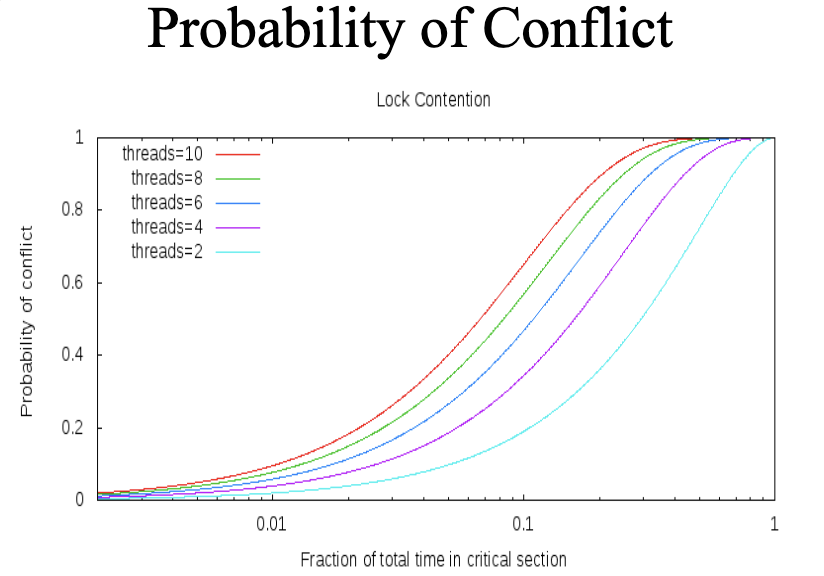
\includegraphics[scale=0.5]{images/contention.png}
% \end{center}
% \exampleEnd

In a FIFO queue formation\footnote{FIFO formation happens when threads wait in line to access the
  resource.}, the formula to estimate the probability of contention is defined as
\[P_\textit{conflict} = 1 - \left(1 - \frac{T_\textit{wait} + T_\textit{critical}}{T_\textit{total}}\right)^{\textit{threads}}\]
  where
  
\begin{enumerate}[label=\textit{(\roman*)}]
\item $P_\textit{conflict}$ is the probability of contention.
\item $T_\textit{wait}$ is the time spent waiting for the resource.
\item $T_\textit{critical}$ is the time spent actively using the resource in a critical section,
  where it has exclusive access.
\item $T_\textit{total}$ is the total time a thread takes to complete its execution, including both
  the time spent waiting(\textit{(ii)}) and the time spent using the resource (\textit{(iii)}).
\item $\textit{threads}$ is the number of threads.
\end{enumerate}
In the general case\footnote{The general case assumes there is no FIFO queue formation.}, we get
\[P_\textit{conflict} = 1 - \left(1 - \frac{T_\textit{critical}}{T_\textit{total}}\right)^{\textit{threads}}\]

In both cases, as contention increases, the probability of contention increases. If
$T_\textit{wait}$ becomes \textit{long enough}\footnote{$T_\textit{wait}$ reaches teh mean
  inter-arrival time.}, newcomers joining the queu can make the wait time even longer, potentially
ceasing parallelism. 

\exampleBegin{The Convoy Effect}
\begin{center}
  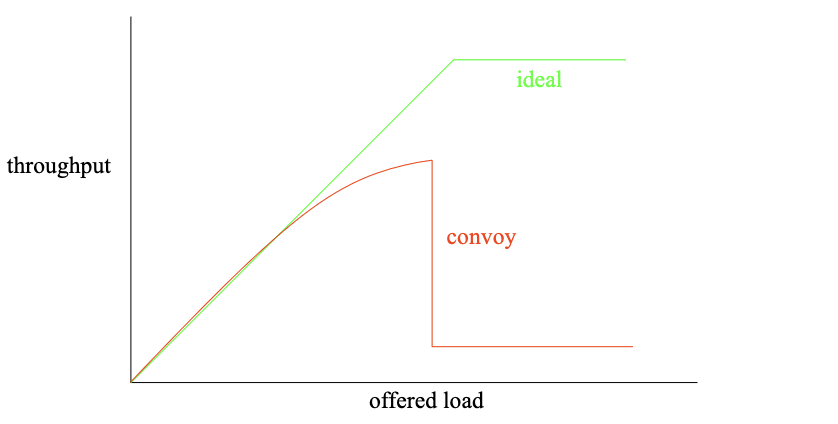
\includegraphics[scale=0.8]{images/convoy.png}
\end{center}

Here we see the graph illustrating the convoy effect. The inflection point of the convoy line
represents the system bottlenecking due to a high $T_\textit{wait}$.
\exampleEnd





\section{Priority Inversion}
\definitionBegin{Priority Inversion}
\textbf{Priority inversion} refers to a situation in priority-based scheduling systems using locks
where a higher-priority process is blocked and delayed by a lower-priority process that currently
has a lock on the desired resource. This effectively reduces the higher-priority process to the
lower-priority process. 
\definitionEnd

Priority inversion can lead to reduced performance, since the program may be bottlenecked by the
lowest-priority process.  This leads to an inefficient utilization of resources and increases the
risk of deadlock, especially with intermediate priorities\footnote{Intermediate priorities may lead
  to a cyclic dependency which will cause a deadlock scenario.}. Moreover, the program becomes
unpredictable and has the potential to cause system crashes.

\exampleBegin{Get on my Level}
Suppose we have two processes, $L$ (low-priority) and $H$ (high-priority) and a mutex $M$. Say $L$
is holding $M$ and is preempted since $H$ has higher priority and is ready to run. However, $H$
blocks for $M$ since $L$ is currently holding it! This reduces $H$'s priority to $L$'s priority. 
\exampleEnd


\subsection{Priority Inheritance}
A common solution to the priority inversion problem is \textit{priority inheritance}. It involves
temporarily raising the priority of the lower-priority task, $L$, (holding the lock) to that of the
highest-priority task waiting for the locked resource, $H$. This prevents $L$ from being preempted
by a higher priority task waiting on the locked resource. Once the resource is released, the
priority of $L$ is reduced to its original value.





\section{Deadlocks}
\definitionBegin{Deadlock}
A \textbf{deadlock} is a situation where two entities are unable to proceed with execution because
they are each waiting for the resource that the other entity holds.
\definitionEnd

Understanding deadlocks are important for a myriad of reasons. They pose a major risk in complex
applications since they can lead to system failures. Moreover, they are usually hard to detect and
their occurrence is usually nondeterministic. Hence, it is usually commonplace to prevent the
possibility of deadlocks at design time.

\exampleBegin{The Dining Philosophers Problem}
Suppose there are 5 philosophers at a table along with 5 plates of pasta and 5 forks. Each
philosopher needs two forks to eat pasta, but must pick them up one at a time. Assume that the
philosophers will not negotiate with one another and they may try to eat at any given moment. Given
these constraints, we see a potential deadlock.

If all 5 philosophers attempt to eat at the same time, each grabs one fork. Since the philosophers
do not negotiate with each other, they wait on another philosopher to 
relinquish a fork. However, since all 5 philosophers are waiting, we see that none of the
philosophers will eat, leading to deadlock!
\exampleEnd

Deadlocks are usually hard to detect since process' resource needs are constantly changing, as they
depend on what data they are operating on, where in computation they are, and what errors have
occurred. Additionally, modern software usually relies on many
\textit{independent}\footnote{Independent: Services need not be aware of others' existence.}
\textit{services}\footnote{Services encapsulate a \textit{lot} of complexity, and as such, we don't
  know what resources they require nor do we know when/how they are serialized.} that each requires
a variety of resources.  


\subsection{Resource Types}
\definitionBegin{Commodity and General Resources}
\textbf{Commodity resources} are ones that are given to processes in \textit{quantities}. They are
usually shareable among processes and can be divided/allocated as needed.
\tcblower
\textbf{General (serially reusable) resources} are ones where processes require exclusive access to
a particular instance.
\definitionEnd


\exampleBegin{Commitment Issues (Over-commitment)}
Suppose you have a system with 8 GB of physical memory and a Virtual Machine that allocates a total
of 16 GB of virtual memory to 4 \textit{VM's}\footnote{In this example, VM will refer to Virtual
  Machines.}. So, each VM thinks it has 4 GB of memory. Now assume that all VM's start using their
allocated memory extensively. As they begin to exceed the amount of physical memory available,
potential deadlocks can arise if the resource manager is not careful.
\exampleEnd

\exampleBegin{Cyclic Dependencies}
Suppose there are two processes A and B and two semaphores X and Y. Now, assume A acquires X and B
acquires Y. A deadlock happens when:

\begin{enumerate}[label=\textit{(\roman*)}]
\item A tries to acquire Y but is blocked since it's being held by B.
\item B tries to acquire X but is blocked since it's being held by A.
\end{enumerate}
So, we have that A and B are both waiting on each other, forming a cyclic dependence. These types of
deadlocks are usually prevented at design time.
\exampleEnd


\subsection{Deadlock Conditions}
\label{subsec:DC}
For a deadlock to occur, \textit{all} four conditions \textit{must} be met:
\begin{enumerate}[label=\textit{(\roman*)}]
\item Mutual exclusion
\item Incremental allocation
\item No preemption
\item Circular waiting
\end{enumerate}


\subsubsection{Condition I: Mutual Exclusion}
The resource in question \textit{must} be one that requires exclusive access; i.e. once a resource
has been given to a process, \textit{all} other requesting processes \textit{must} wait. Otherwise,
we wouldn't have deadlock since we can just give an instance of the resource to all the requesting
processes. 


\subsubsection{Condition II: Incremental Allocation}
Entities are allowed to ask for resources at any time rather than requesting them before
execution. Otherwise, they either get everything they need and run to completion or don't get
everything they need and abort execution. In either case, we don't get deadlock.


\subsubsection{Condition III: No Preemption}
When an entity has access to a resource, we cannot preempt it; i.e. once an entity has access to a
resource, we must wait for it to free the resource. Otherwise, we can resolve all deadlocks by preempting the
offending process(es). 


\subsubsection{Condition IV: Circular Waiting}
We \textit{must} have a situation that causes a circular wait; i.e. we have a cycle in a graph of
resource requests. Otherwise, there is no cycle, so \textit{someone} can complete without anyone
releasing a resource. This allows even a long chain of dependencies to
\textit{eventually}\footnote{We promise that it eventually unwinds, not that it unwinds quickly.} unwind.


\subsection{Avoiding Deadlock: The Reservation System}
Note how we said in the previous section that \textit{all} four conditions must be met for a
deadlock to arise. However, that is much easier said than done. We can, however, use methods that
guarantee that no deadlock can occur by nature. We introduce the notion of \textit{reservations}.

In the reservation system, the resource manager tracks outstanding reservations requested by
processes. Rather than fulfilling any and all requests, we only honor reservations if and only if
the resources are truly available. This prevents situations where too many tasks expect resources
that aren't there (over-commitment), detecting over-subscriptions early.

In the reservation system, we may run into resource starvation. Because reservations are only
honored if the resource is available, some processes may never receive the resources they
reserved. While this leads to resource scarcity, it does \textit{not} lead to a deadlock! This
allows us to handle this scarcity in a \textit{controlled} way.

We clearly face a dilemma: should the resource manager over-commit or under-utilize? Striking a
balance is key to maintain optimal resource utilization without risking critical resource shortages.


\subsubsection{Handling Reservations}
Entities seldom require \textit{all} available resources at all times. As a corollary, we
extrapolate that all clients don't need their maximum allocated resources simultaneously. This
raises the question: Can we \textit{safely} over-book resources.

\exampleBegin{Fly Fucked}
Airplanes often over-book on every flight, banking on people not showing up. Fortunately for them,
they are often correct! Can we apply the same concept to operating systems?
\exampleEnd

Let's define what a safe allocation is:

\definitionBegin{Safe Allocation}
A \textbf{safe allocation} is one where everyone can \textit{eventually}\footnote{Again, we only
  promise that all entities eventually complete, not that they complete in a swift manner.} complete
their tasks. That is, we ensure that no deadlocks!
\definitionEnd

\corollaryBegin{Commodity Resource Management in Real Systems}
Many real-world systems use advanced reservations to manage resource efficiently. In these systems,
one a reservation is accepted, the system is obligated to honor it. This way, we prevent resource
starvation since allocation failures only occur at the time of reservation, usually before the start
of execution. This makes system behavior more predictable and easier to handle. This also forces the
client to deal with the reservation failure, meaning we don't have to!
\corollaryEnd


\subsection{Reservation Failures}
While reservations eliminate deadlock, applications still need to deal with reservation failures. We
should design applications to handle failures \textit{gracefully}\footnote{For example, we can
  refuse to perform a new request, but continue running.}. Additionally, we need to be able to
communicate to the requester that a reservation failed (e.g. error messages or return
codes). Finally, the application \textit{must} be able to continue running. Naturally, this forces
all critical resources to be reserved prior to execution.

While rejecting requests are not ideal, they are better than system failure later down the
road. This way, the advanced notice allows applications to adjust their services to work without the
unavailable resource. If the application is in the process of fulfilling a request and the resource
becomes unavailable, complications arise. At this point, if a failure occurs, we need to roll back
the actions that have already taken. This process can be complex or even impossible depending on the
situation.

\exampleBegin{Reservation Rejected!}
Consider a web server that relies on a database. If the database becomes temporarily inaccessible
(e.g. maintenance or network issues), we can adjust our services to display a cached version of the
web page or show an error message instead of crashing entirely! We can do this by implementing
mechanisms like graceful degradation. Let's look at an example of a situation where a reservation is
rejected in the middle of fulfilling a request. Suppose we have a shopping application is processing
a customer's order, and the payment gateway becomes inaccessible between deducting funds and
confirming the order. Here, we need to refund the money which would be a nontrivial task.
\exampleEnd


\subsection{Avoiding Deadlock: Additional Measures}
Deadlock prevention focuses on ensuring that a specific lock doesn't lead to deadlock by addressing
one of the four deadlock conditions (See \refto{subsec}{DC}). Remember, if \textit{any} of the four
conditions are not met, we don't have deadlock! Let's take a look at how we can prevent deadlock by
failing to satisfy each of the four conditions.


\subsubsection{Condition I: Mutual Exclusion}
We can prevent deadlock by utilizing shared and private resources. Recall that deadlocks cannot
occur over shareable resources, which are typically managed using atomic instructions. Like
shareable resources, deadlock cannot occur over private resources since they are owned by individual
processes!

\subsubsection{Condition II: Incremental Allocation}
To combat deadlock, we can allocate all our resources in a single operation as well as use
non-blocking requests. Here, if we cannot allocate everything, we return failure and don't
lock, proceeding otherwise. Note that in this approach, we get an all or nothing
allocation. Non-blocking requests will fail if the request cannot be satisfied immediately. Finally,
we can disallow blocking while holding resources. That is, we must release all held locks before
blocking, reacquiring them \textit{after} you return\footnote{It is important to note that while this
approach may solve the deadlock problem, it can introduce new ones. Remember, CS is all about give
and take!}.


\subsubsection{Condition III: No Preemption}
We can implement resource confiscation to combat deadlocks. Here, we seize and reallocate resources
from existing processes. We achieve this via resource ``leases'', with time-outs and ``lock
breaking''\footnote{Lock breaking: When a process' ``lease'' is up, the resource is automatically
  taken away and returned to the resource pool.}. This approach requires us to enforce resource
revocation. We can do this by either invalidating resource ownership \textit{(i)} or terminating the previous
owner \textit{(ii)}. To achieve \textit{(i)}, when a resource is taken away from a process, the
ownership of that resource is invalidated. Thus, the process loses access to the resource and
prevents it from attempting to use a confiscated resource! To achieve \textit{(ii)}, we simply
terminate the previous owner. This option is usually a last resort and is only used when resource
invalidation is not possible\footnote{Like Condition II, lock breaking may fix deadlock but can
  damage resources!}.


\asideBegin{Seizing Resources}
The operating system can only seize a resource if the process has to use a system service to access
the resource. If the process has direct access to the object (e.g. the object is part of the
process' address space), then we're fucked and usually have to resort to terminating the process to
free the resource.
\asideEnd


\subsubsection{Condition IV: Circular Waiting}
We can enforce \textit{total resource ordering}. Here, all processes requesting resources follow the
same order when allocating them. Given two resources $R_1$ and $R_2$, \textit{all} processes are
\textit{required} to allocate $R_1$ before attempting to allocate $R_2$. This way, we prevent
circular dependencies by creating a DAG\footnote{DAG: Directed Acyclic Graph}! To implement total
resource ordering, we need to order the resources! We can do this by ordering them by resource type
(e.g. groups before members) or by relationship (e.g. parents before children).

\asideBegin{The Lock Dance}
Suppose two process ($P_1$ and $P_2$) needs to allocate resources ($R_1$ and $R_2$) out of
order. Initially, we have $P_1: R_1$ and $P_2: R_2$, but our desired state is $P_1: R_2$ and $P_2:
R_1$. Let's do the lock dance!

\begin{enumerate}[label=\textit{(\roman*)}]
\item $P_1$ releases $R_1$ ($P_1:\O$, $P_2: R_2$)
\item $P_2$ releases $R_2$ ($P_1:\O$, $P_2: \O$)
\item $P_2$ acquires $R_1$ ($P_1: R_2$, $P_2: \O$)
\item $P_1$ acquires $R_2$ ($P_1: R_2$, $P_2: R_1$)
\end{enumerate}
\asideEnd


\subsubsection{Conclusion}
There is no universal solution to all deadlocks. Determining which solution to use is on a
case-by-case basis, and fortunately for us, we only need to implement one of the four!


\subsection{A Deadlock ``Solution''}
We can also elect to simply ignore the problem. In many cases, deadlocks are \textit{very}
improbable and implementing any of the solutions provided above can be very expensive. So, we can
just forget about them and pray to the CS gods that we don't run into a deadlock.


\subsubsection{Deadlock Detection and Recovery}
We can allow deadlocks to occur, but we want to be able to detect them once they occur (the sooner
the better). Once we detect them, we need a method of breaking them to continue execution. Whether
or not this is a good idea depends.

In general, it's probably a more practical approach since the
overhead and complexity of deadlock-proofing your system may be too expensive. However, in critical
systems where resource availability is crucial (e.g. real time systems), we might want to invest the
time and energy into preventing deadlocks, since they can lead to severe disruptions, data loss, or
even safety hazards.


\subsubsection{Implementing Detection}
We can implement deadlock detection by using a wait-for graph or an equivalent data structure. When
a lock request is made, the system updates the wait-for graph and checks for the presence of a
deadlock (cycle detection).

Whether or not it's better to reject a lock request (that will lead to deadlock) and not let the
requester block depends. If we reject a lock request, there's no deadlock, but it might result in
process disruptions and inefficiencies. If we allow the requester to block, we may get deadlock, but
the system will be more resource-efficient overall. 

Implementing detection may be challenging however, since we need to identify \textit{all} resources
that can be locked.


\subsubsection{Application Level Deadlocking}
Some applications include their own internal locking mechanisms independent of the operating
system. Since the OS doesn't know about these locks, it cannot offer any help. Here, deadlock
detection may be appropriate since the application itself has the necessary information to identify
and handle deadlocks.


\section{Health Monitoring}
Not everything is a deadlock! There are a lot of reasons systems hang and make no
progress. Occasionally, it really is a deadlock. Other times, it's something else (e.g. live-lock,
lock flaws, etc.). If there are no locks, it's definitely not deadlock. Even if there are, it may
not necessarily be deadlock.

We can use service/application \textit{health monitoring} in lieu of deadlock detection. Here, we
monitor application progress and submit test transactions. If responses take \textit{too
  long}\footnote{Too long is subjective and is dependent on the system requirements.}. Health
monitoring is much easier to implement than deadlock detection and can detect a wider range of
problems, including (but not limited to):

\begin{enumerate}[label=\textit{(\roman*)}]
\item Live-lock: A process is running but unable to proceed due to unmet dependencies.
\item ``Sleeping Beauty'': A process waits indefinitely for an event(s) that will never happen.
\item Priority inversions: Health monitoring can detect when priority inversions cause system
  hangups!
\end{enumerate}


\subsection{Monitoring Process Health}
We can use a variety of metrics to determine process health. We will cover:
\begin{enumerate}[label=\textit{(\roman*)}]
\item Obvious Failures
\item Passive Observation
\item External Monitoring
\item Internal Instrumentation
\end{enumerate}


\subsubsection{Obvious Failures}
We can actively check for obvious failures like abnormal process exits or core dumps. These
indications can be monitored and analyzed to identify the cause of failure.


\subsubsection{Passive Observation}
We can identify processes that are unresponsive or hanging by monitoring CPU usage, blocking status,
and network/disk I/O. If a process is not consuming CPU time or blocked for extended periods of time, it may be
stuck. Likewise, if a process is not performing expected I/O operations or engaging in network
activities, it may potentially be stuck.


\subsubsection{External Monitoring}
We can interact with processes to asses their responsiveness. Common techniques are pings, null
requests, and standard test requests. We can ping the process to measure response time. If the
process fails to respond within a given time frame, it may be unresponsive. Like pings, we can send
a null/dummy request expecting acknowledgment by the process. Lack of acknowledgment can indicate
unresponsiveness. More specifically, standardized test requests expect specific responses from the
process. Failure to provide the expected response may trigger alerts.


\subsubsection{Internal Instrumentation}
We can embed monitoring and testing directly within the codebase of the process via white box
audits, exercisers, and continuous monitoring. White box audits involve reviewing internal code and
data structures to identify potential vulnerabilities, inefficiencies, or errors. Exercisers are
designed to simulate various scenarios to stress-test the process, which can help uncover unexpected
behavior and/or vulnerabilities, particularly in complex systems. Continuous monitoring keeps track
of key performance metrics and states within the process. Monitoring tools collect data and trigger
alerts when the numbers deviate from the expected behavior.


\subsection{Unhealthy Processes}
When processes are unhealthy, killing and restarting any and all affected software is a common and
easy recovery strategy. However, deciding which processes to kill and restart requires a balance
between addressing the issue and minimizing disruptions.

It is important to note that unresponsive processes may not necessarily be the cause of the
problem. Thus, we need to take into consideration how kills and restarts can impact current clients
which are dependent on service API's and protocols. Applications must be designed to handle
different types of restarts: cold, warm, or partial. In highly available systems, restart groups are
well-defined and specify the groups of processes to be restarted together as well as inter-group
dependencies.


\subsection{Failure Recovery}
\definitionBegin{Cold Restart}
A \textbf{cold restart} involves terminating the entire process and restarting it from
scratch\footnote{This ensures a clean slate but may incur longer downtime.}
\definitionEnd

\definitionBegin{Warm Restart}
A \textbf{warm restart} involves restarting the process but maintaining existing
connections/sessions\footnote{This minimizes disruption but may not solve the problem.} 
\definitionEnd

\definitionBegin{Partial Restart}
A \textbf{partial restart} involves restarting only specific components of the process$^a$.
\definitionEnd

The failure recovery methodology involves retries, rollbacks, and continued functionality. First, we
retry a request (if possible), but set limits on how many/how long we wait. If a request ultimately
fails, we want to roll back failed operations to before the request and return an error. Finally, we
continue with reduced capacity/functionality, accepting only requests we can handle, rejecting
otherwise. Additionally, we implement automatic restarts (cold, warm, partial) and use escalation
mechanisms to address failed recovery attempts.


\subsection*{Interlude: Making Synchronization Easier}
\addcontentsline{toc}{subsection}{Making Synchronization Easier}
Locks, semaphores, and mutexes are hard to use correctly, since they may not be used when they're
needed, may be used incorrectly, and may lead to deadlock or other hanging situations.

One way we can make synchronization easier is to automate the generation of serialization
mechanisms. Here, shared resources (objects with methods that require serialization) are
identified. Code is written to operate on shared resources without \textit{explicitly} adding
synchronization. The compiler then generates the required locking and releasing mechanisms to ensure
proper serialization.





\section{Monitors}
\definitionBegin{Monitors}
\textbf{Monitors} are objects with built-in synchronization mechanisms.
\definitionEnd

We introduce the concept of monitors as protected classes. Here, each monitor object is associated
with a mutex that is automatically acquired when a method is invoked on the monitor and released
upon method return. Monitors provide encapsulation, allowing developers to manually avoid
identifying critical sections, and clients are relieved of the responsibility of managing locks.


\subsection{Simplicity v. Performance}
Monitors provide simplicity in synchronization by automatically locking the \textit{entire} object
during method invocations. Since objects are locked for the entire duration of any method
invocation, it is a conservative approach to synchronization and can potentially lead to performance
issues. Locking the entire object can eliminate parallelism and create the potential for thread
contention, resulting in convoys (See \refto{subsec}{TCE}). When implementing synchronization
primitives, we consider the trade-offs of simplicity v. performance. Fine-grained locking is
difficult and error prone, but often performs well while coarse-grained locking may be simpler to
implement, but can create bottlenecks.


\subsection{Java's Synchronized Methods}
In Java synchronized methods, each object has an associated mutex and is acquired for specified
synchronized methods. Here, not \textit{all} methods need to be synchronized; synchronization is
needed only for the methods with access to shared resources. The mutex is automatically released
upon the \textit{final} return of the synchronized method.

Here, nested calls by the same thread do not reacquire the mutex, avoiding unnecessary locking and
unlocking. Static synchronized methods lock the class-level mutex, affecting all instances of the
class. Advantages include finer lock granularity and a reduced risk of deadlocks, but the cost
usually involves the responsibility of developers to \textit{correctly} identify which methods need
synchronization.










\part{Persistence}
\chapter{Devices and Device Drivers}
\section{Overview}
This chapter covers the OS's role in properly handling devices via device drivers.

\definitionBegin{Peripheral Device}
A \textbf{peripheral device} is an external device that is attached to the computer to perform
specific functions.
\definitionEnd

Each peripheral device has code associated with it for performing operations and integration into
the system. In modern commodity operating systems, the amount of code dedicated to handling devices
is substantial and can outweigh other parts of the system's codebase!

Peripherals are usually connected to the computer via a bus, which facilitates communication between
peripherals and other system components. They are designed to perform specific (usually predefined)
functions rather than independently executing arbitrary computations. The system sends a signal on
the bus to instruct the peripheral to perform its designated task, which is then performed asynchronously
alongside other system activities. Once finished, the signal is sent back from the peripheral to the
system on the bus to communicate the results of the operation.

\section{Devices and Performance}
Compared to the CPU, bus, and RAM, most peripheral devices are \textit{slow}\footnote{Sometimes
  several orders of magnitude slower than the CPU, bus, or RAM.}. Consequently, managing devices
\textit{efficiently} presents performance challenges. The system operates at the speed of the CPU,
bus, and RAM, but correct behavior often requires interactions with \textit{slow}$^1$ devices. Thus,
it is up to the system to effectively manage the discrepancy in speed to ensure accurate
functionality and optimal performance!

\subsection{Why the Operating System?}
Peripheral devices are often managed by the operating system rather than user-level code for various
reasons.


\subsubsection{Criticality for Correctness}
Certain devices are integral to the proper functioning and correctness of the entire system.

\exampleBegin{Flash Drives}
A flash drive that holds swap space is crucial for efficient memory management, an OS service (See
\refto{chap}{MM})! Managing such critical resources requires coordination and control at the OS
level to ensure reliable operation.
\exampleEnd


\subsubsection{Shared Access}
Many devices must be shared among multiple processes which requires OS-level control! Managing
shared access in a fair and efficient manner requires sophisticated synchronization mechanisms and
resource allocation strategies.


\subsubsection{Complexity}
Handling shared resources involves intricate resource management (including locking, queuing, and
prioritization). Such complexity is beyond the capabilities of user-level code and requires OS-level
control.


\subsubsection{Security}
Certain devices have security implications, and as such we need a trusted system to manage them. Oh
look, the OS \textit{is}\footnote{should*} be trusted!

\exampleBegin{Network Interfaces}
Network interfaces that handle communication between applications and external
systems require OS-level control to ensure a secure channel for communication.
\exampleEnd





\section{Device Drivers}
\definitionBegin{Device Driver}
A \textbf{device driver} is specialized software that acts as a bridge between a computer's OS and
specific hardware (peripheral) devices, enabling communication and interaction between software and
hardware components.
\definitionEnd

Device drivers enable us to interface with the device from the application layer! When we need to
interact with the device, we send a signal to the OS which will in turn call the appropriate device
driver. The device driver then feeds detailed instructions to the hardware, performing the desired task.

Code for hardware devices is usually specialized to their unique functionalities. The code serves as
a \textit{driving} force behind the device, enabling it to carry out its intended operations. Thus,
each hardware device within a system usually has its own driver (code segment).


\subsection{Properties}
Let's take a look at typical properties of device drivers. They are:

\begin{enumerate}[label=\textit{(\roman*)}]
\item Device drivers are highly specific to the particular hardware device(s) they are meant to
  support.
\item Device drivers are inherently modular, allowing them to be developed and maintained independently.
\item Device drivers typically interact with the rest of the system via limited and well-defined
  (see \textit{(i)}) interfaces, promoting compatibility and predictable behavior.
\item Correctness is paramount to a device drivers' utility since it affects both the accuracy of
  the operation it implements as well as the system as a whole.
\item Device drivers are often developed by programmers with an in-depth understanding of the
  \textit{specific}\footnote{Note that these developers may not be experts in the broader system, but they
    need not worry about that (see \textit{(ii)}).} device's functionality.
\end{enumerate}


\subsection{Abstractions}
Let's abstract away device drivers!

\abstractionBegin{Driver Abstractions}
We define an idealized class of devices, an \textit{abstraction} over device drivers. These classes
define expected behavior/interfaces that the drivers will support.
\abstractionEnd

These abstractions over device drivers provide a structured way to interact with a diverse set of
hardware devices. Mainly, it lets device drivers to adhere to a common framework by abstracting
device-specific complexities. Further, they regularize and simplify the interaction between software
(applications) and hardware (devices).

As with any abstraction, driver abstractions encapsulate the knowledge of how to use devices
effectively, translating standard operations we interface with into device-specific
actions. Consequently, they provide a consistent and intuitive interface for users and ensure proper
coordination between devices and software. Furthermore, we have fault handling embedded in
abstractions, guiding the handling of recoverable device-level faults and avoiding their escalation into
system-wide faults.


\subsection{Generalizing Abstractions}
At first glance, it may seem that each device deserves its own unique driver. But upon closer
inspection, we can see that there are many commonalities between them, particularly among classes
of devices.

\exampleBegin{Class of Devices}
Let's look at the class of flash drives. Here, we see that \textit{all} flash drives utilize NAND
flash memory to store data. We can leverage commonalities such as the NAND flash memory to build an
abstraction layer atop the \textit{class} of flash drives.
\exampleEnd


\subsection{Providing Abstractions}
The OS will define device \textit{classes} (e.g. flash, display, printer, etc.). These classes
define the expected interfaces/behavior; i.e. \textit{all} drivers in the class supports
\textit{all} the standard methods defined by the OS. 





\section{Interfaces}
\subsection{Device Driver Interface}
\definitionBegin{Device Driver Interface}
The \textbf{device driver interface (DDI)} is a standardized set of top-end entry points that
connect the operating system with device drivers.
\definitionEnd

The DDI serves as a basis for device-independent applications and enable the system to seamlessly
integrate new devices. It plays a critical role in providing a contract for third-party developers
and is composed of entry points that align with syscalls (like \texttt{open()}, \texttt{close()},
\texttt{read()}, \texttt{write()}) and OS frameworks (like block I/O for flash drivers or network
protocols for network drivers).


\subsection{Driver/Kernel Interface}
\definitionBegin{Device/Kernel Interface}
The \textbf{device/kernel interface (DKI)} is the specification of bottom-end services provided by
the operating system to device drivers.
\definitionEnd

The DKI outlines the functionalities that drivers can request the kernel to perform, similar to an
ABI (See \refto{sec}{ABIS}). It is essential for the DKI to be well-defined and stable to facilitate
teh development of third-party drivers and to ensure backwards compatibility. Each OS has its own
DKI, but they are all similar.

\exampleBegin{``You'll Never Find Someone Like Me''}
All DKI's provide functionalities like memory allocation, data transfer and buffering, I/O resource
(ports, interrupts, etc.) management, DMA, synchronization, error reporting, dynamic module support,
configuration, plumbing, and more!
\exampleEnd

\exampleBegin{Linux Device Driver Abstractions}
Linux takes inspiration from older Unix systems and organizes devices into several super-classes
(e.g. block, character, (potentially) network devices). Each super-class defines a set of common
behaviors and interfaces for device drivers. This classification allows Linux to provide a
structured framework for various types of device drivers and enhances code reusability.

Classes provide a good organization for abstraction since they provide a common framework to reduce
the amount of code required for each new device. However, it is important to note that a
\textit{lot} of driver functionality is specific to the device, implying that class abstractions
don't cover \textit{everything}, but are rather used to ensure all devices in a class provide
certain minimal functionalities.
\exampleEnd

\section{Device Drivers in Operating Systems}
There are usually a \textit{lot}\footnote{A Linux 2.6 kernel came with over 3200 drivers!} of device
drivers in a system, most of which are relatively independent. So, a pluggable model is commonly
used to integrate device drivers into the OS, especially since we may need to add more device
drivers in the future. The operating system provides mechanisms that enable users to plug in
specific drivers in well-defined ways, simplifying the process of modifying, updating, and/or
expanding driver support in the OS.


\subsection{Layering Device Drivers}
Device drivers have multiple layers reflecting different levels of interactions and
functionality. At the lowest layer we have interactions with the bus. Here, we have standardized
processes for addressing devices, signaling coordination, and data transfers. Interactions at this
level are relatively independent of the specific devices that are in use. At the highest layer, we
have relatively standardized interactions, often involving file-oriented approaches for
communication. Between these two layers, we have device-specific interactions which accommodate the
unique behaviors and features of individual devices. These layers allow for a modular development,
encapsulation of device-specific complexities, and separation of concerns!


\subsection{Device Driver Code Operating Systems}
While device driver code \textit{can} be integrated into the operating system, we often distribute
code based on the functionality it brings. Common functionalities like caching, file systems code
(independent of a particular device), and network protocols (above physical/link layers) are best
suited to be part of the operating systems. Conversely, specialized functionalities that differ
between devices are better suited for device drivers.

\exampleBegin{Graphics Drivers}
Suppose we want to write code for a particular brand of graphics card. The intricacies of managing
\textit{unique}\footnote{Suppose we need to implement hardware-accelerated shading using the
  graphics card's highly parallelized architecture...} graphics card's functionalities would be
confined to its respective driver, whereas a functionality like display resolution/screen layout
management would be reserved to the operating system, since any graphics card worth its money
supports that functionality.
\exampleEnd





\section{Devices and...}
\subsection{Interrupts}
\label{subsec:INTER}
Devices in operating systems rely heavily on the interrupt-driven model for communication and
coordination. It is important to note that drivers are not treated as processes and therefore not
scheduled. Since they work at a (much) slower speed than the CPU, drivers typically perform their
tasks independently while the CPU engages in other activities. Interrupts are then used to alert the
CPU and gain its attention when they require processing.

\subsection{Buses}
Devices are not directly connected to the CPU. Instead, both the CPU and devices are connected to a
bus (which can be the same or differ between the two). Devices communicate with the CPU via the bus
for both sending and receiving interrupts as well as for transferring data and commands.

Devices signal the controller when they are done/ready. When the device finishes, the controller
puts an interrupt on the bus, which then transfers it to the CPU.


\asideBegin{CPU's and Interrupts}
Note that interrupts are similar to traps! Traps come \textit{from} the CPU, whereas interrupts are caused
externally \textit{to} the CPU. Unlike traps, interrupts can be en/disabled by special CPU
instructions. That is, devices can be told when they may generate interrupts. Furthermore,
interrupts may be held \textit{pending}\footnote{Pending state: The interrupt is recognized
  by the system but is not immediately serviced by the CPU.} until the software is ready for it.
\asideEnd





\section{Device Performance}
This section explores how we can efficiently utilize the devices in our system.


\subsection{Good Device Utilization}
\label{subsec:GDU}
Recall that key devices, such as those handling file I/O and network communication, are notably
slower than the CPU. When these devices are underutilized and remain idle, their throughput drops,
which in turn can lead to lower overall system throughput, longer service queues, and slower
response times. The consequences of such inefficiencies are reflected in degraded system performance
and a less responsive user experience.

It is critical to strike a balance between high level of activity for these key devices and reducing
CPU wait time. A common strategy is to start request $n + 1$ immediately after request $n$ finishes.

\exampleBegin{Device Delays}
Suppose we have a real time system that interfaces with several devices.  Delays in device
utilization can disrupt real-time data flows, resulting in unacceptable performance numbers and
potential data loss!
\exampleEnd

How do we achieve good device utilization? Parallelism! Since devices operate independently of the
CPU, they can operate in parallel with the CPU. However, one key challenge is how to address a
situation where both the device(s) and CPU need to access shared memory (RAM). It is essential to
manage and coordinate access to RAM to prevent conflicts, ensure data consistency, and optimize
system performance.

\asideBegin{CPU Caching}
Modern CPU's try to avoid going into RAM by utilizing registers and on-chip caches to store and
retrieve frequently used data and instructions quickly. By minimizing the number of trips to RAM
(sometimes referred to as a cache hit), the CPU can operate at much faster speeds and achieve better
performance.
\asideEnd

CPU caching frees up the memory bus for devices to use, offloading some of the bus-related
activities from the CPU and potentially improving system performance. We need to balance memory bus
usage between devices and the CPU to avoid contention and ensure optimal parallelism.


\subsection{Direct Memory Access}
\definitionBegin{Direct Memory Access}
\textbf{Direct Memory Access (DMA)} allows two \textit{devices}\footnote{These devices must be
  attached to the memory bus.} to transfer data directly between each other without involving the
CPU as an intermediary.
\definitionEnd

While DMA offers efficient data transfer, it also limits the memory bus; the memory bus can only be
used for one purpose at a time, so if DMA is active, it's not servicing the CPU. Fortunately, the
CPU usually doesn't require bus access during DMA operations. DMA enables data to e moved from a
device to memory at the speed of the bus/device/memory, bypassing the CPU. 


\subsection{Keeping Devices Busy}
Recall that we want to keep key devices busy and optimize their utilization within the OS (See
\refto{subsec}{GDU}). We can do this by utilizing several techniques.


\begin{enumerate}[label=\textit{(\roman*)}]
\item We can allow multiple pending requests at the same time by queuing them, similar to how we put
processes in a ready queue.
\item We can utilize DMA for data transfers to minimize delays and overhead on the CPU.
\item We can coordinate the process of handling completed requests via interrupt-driven mechanisms
  (See \refto{subsec}{INTER} and \refto{subsec}{GDU}).
\end{enumerate}


\subsection{Transfer Size}
Bigger data transfers are non-trivially more efficient than smaller transfers. This is because data
transfers come with inherent overhead per operation, including factors like DMA, device-specific
tasks, and OS involvement. Overhead activities involve setting up the transfer, initiating new
operations, and handling completion interrupts. Thus, larger data transfers are more efficient since
they have lower overhead per byte! These efficiency gains are not limited to software and extend to
hardware and other contexts as well! The principle of reduced overhead per byte is a fundamental
aspect of optimizing data movements and resource utilization.


\section{I/O and Buffering}
\definitionBegin{Buffer}
A \textbf{buffer} is a temporary storage area used to hold data that is ready to be processed or
transferred.
\definitionEnd

Recall that I/O requests involve transferring data between memory and devices. Data that is part
of I/O operations is stored in memory locations called buffers. Buffers play a key role in
facilitating efficient data movement and communication between devices and memory (especially in
I/O). They usually contain data that is ready to be sent to a device or is awaiting data from a
device.

An essential aspect of buffer management is ensuring that buffers are available when devices are
prepared to use them. The OS is responsible for coordinating the availability of buffers to ensure
smooth data transfers.

\subsection{Buffering Issues}
While fewer and larger data transfers are more efficient for I/O operations, they may not
necessarily align with application requirements since natural record sizes are often small. The
operating system can address this issue by employing various buffering strategies.

We can consolidate I/O requests to optimize data transfers by maintaining a cache of recently used
disk blocks, enhancing the efficiency of subsequent operations. For small write operations, the OS
accumulates the data and flushes it out as blocks fill up, minimizing the overhead associated with
frequent writes.

When reading data, the OS reads entire blocks and delivers the requested data from the cached
blocks, enhancing read performance. Further, we can employ read-ahead; the OS anticipates upcoming
read operations and proactively reads/caches blocks that have not yet been requested.


\subsection{Deep Request Queues}
Deep request queues refer to when we have a large number of queued I/O operations. Maintaining such
a queue helps keep the device(s) busy, minimizing idle time. For example, deeper queues also contribute to
reducing mean seek distance and rotational delay in disk-based devices. Furthermore, adjacent requests may be
combined in the queue, optimizing data transfers. In some cases, certain write operations can be
avoided or optimized via efficient queue management.

We can achieve a deep request queue in a multitude of ways: we can have many entities make requests,
individual processes make parallel requests, read-aheads, and write-back cache flushing.


\subsection{Scatter/Gather I/O}
Since user buffers are paged in virtual memory, buffers may be spread all over physical memory!
Scatter/gather I/O is when we read from/write to multiple page frames, allowing data to be
efficiently transferred between user buffers and devices. There are three basic approaches to
address scatter/gather I/O:

\begin{enumerate}[label=\textit{(\roman*)}]
\item Copy all user data into a physically contiguous buffer.
\item Split logical requests into chain-scheduled page requests.
\item Utilize teh I/O MMU to automatically handle scatter/gather operations.
\end{enumerate}

\subsection{Memory Mapped I/O}
Memory-mapped I/O is an alternative to DMA, and is used for certain types of devices. While DMA is
designed for large contiguous transfers, they may not be the best fit for devices requiring
frequent, small, sparse transfers. Memory-mapped I/O treats registers or memory in a device as part
of the regular memory space, accessible through memory operations.

\exampleBegin{Display Adapters}
This approach is particularly relevant for devices like bit-mapped display adapters, enabling
efficient updates to displays with low overhead and no interrupts. Here, each word of memory
corresponds to one pixel on the display. Applications can use ordinary memory stores to update the
display, simplifying programming and providing efficient access to device-related memory.
\exampleEnd










\chapter{File Systems}
\section{Overview}
Persistent data storage is essential for retaining data across reboots and power downs. Even the
operating system relies on persistent storage to maintain its state! There are several options for
persistent storage: raw storage blocks, databases, and file systems.

\subsection*{Raw Storage Blocks}
Using raw storage blocks involves storing data directly on storage devices like hard disks or flash
drives without any \textit{structure}. While this approach is flexible when it comes to data layout,
it's not very user-friendly and is hard to manage due to its low-level nature.


\subsection*{Databases}
Databases provide a \textit{structured} way to store and manage persistent data. They offer features
like data organization, indexing, and querying, making them good for structured data
management. However, databases often come with overhead and complexity, especially when the data
organization is more straightforward, leading to a bloated system.


\subsection*{File Systems}
File systems offer an organized and \textit{user-friendly} approach to structuring
persistent data. They provide a hierarchy of directories and files, making it intuitive for users
and programmers to store/retrieve data. File systems also manage metadata, permissions, and access
control. This option strikes a balance between raw storage blocks and databases, and is what we will
be focusing on in this chapter.

\definitionBegin{File}
A \textbf{file} is a self-contained entity that can store various types of data (e.g. documents,
spreadsheets, messages, programs, etc.).
\definitionEnd

The basic idea of a file system is to organize data into coherent units, each of which are referred
to as a \textit{file}. The primary goal of a file system is to provide efficient access to files and
a powerful organizing principle for managing the collection of files.


\subsection{File Systems and Hardware}
File systems are typically stored on hardware that provides persistent memory (e.g. flash), with the
expectation that files stored in a particular location (on flash for example) will remain there
between access instances.

For optimal performance, file systems should also be implemented with the underlying hardware in
mind for optimal performance while also striving for cross-hardware compatibility.

\exampleBegin{Flash Drives}
The flash drive is a solid state persistent storage device; i.e. it has no moving
parts. Reads/writes are fairly \textit{fast}\footnote{Reads up to 100 MB/sec, writes up to
  40MB/sec.}, but a given block can only be written once. Writing over a block requires erasing,
which is slower and involves erasing larger sectors of the drive.
\exampleEnd


\subsection{Data v. Metadata}
\definitionBegin{Data and Metadata}
\textbf{Data} refers to the content that a file is intended to store (e.g. text, images, program
instructions, etc.).
\tcblower
\textbf{Metadata} refers to information about the file (e.g. attributes like file size, creation
date, permissions, etc.).
\definitionEnd

Both data and metadata need to be stored persistently within the file system. Typically, data and
metadata are stored on the same storage hardware to ensure that both are accessible together.

\asideBegin{Uniform Functionality}
File systems should be designed to function uniformly across various storage media. This enables the
same program to interact with the file system regardless of the storage medium being used
(e.g. flash v. disk), enhancing program portability and reducing
\textit{complexity}\footnote{Complexity of adapting programs to different storage technologies.}. By
maintaining a consistent interface, the file system can seamlessly manage different storage media
without requiring major changes to program code!
\asideEnd


\subsection{Properties}
Properties we want in a file system include (but are not limited to):

\begin{enumerate}[label=\textit{(\roman*)}]
\item Persistence: The file system should ensure that data and metadata are stored persistently even
  between power cycles.
\item Easy Use Model: The file system should be user-friendly for both accessing individual files
  and organizing collections of files.
\item Flexibility: The file system should not impose limits on the number of files, file sizes,
  types, or contents, allowing users to manage diverse data.
\item Portability: The file system should be able to function consistently across different hardware
  device types, ensuring program portability.
\item Performance: The file system should be robust and dependable, minimizing the risk of data loss/corruption.
\item Security: The file system should incorporate appropriate security measures to protect data
  from unauthorized access or tampering.
\end{enumerate}

\asideBegin{Issues}
There are some concerns we should bring to light before continuing the discussion on file systems:

\begin{enumerate}[label=\textit{(\roman*)}]
\item Performance: Ideally, we would like our file system to be as fast as things like the CPU, bus,
  and memory. However, these devices operate at \textit{nanoseconds} today, and flash drives are
  roughly 1000x slower. This implies that we need to do some \textit{serious} work to hide the
  mismatch in performance speeds.
\item Reliability: Trivially, persistence implies reliability; we want our files to be there when we
  check, \textit{no exceptions}. This implies our file system needs to be free of errors on both the
  hardware \textit{and} software side, the latter of which may be hard to ensure (see
  \refto{part}{C}).
\item Security: We want to ensure controlled and well-defined access to data; i.e. data owners
  should have the ability to determine who has access to their data via an access control model and
  mechanism. We need \textit{strong} guarantees that the system will enforce owners' desired
  controls, implying we'll need to check permissions on access. But remember, we need to strike a
  balance with \textit{(i)}. 
\end{enumerate}
\asideEnd

File systems are built using multiple layers of abstraction. At the top, applications interface with
and access \textit{files}. At the bottom, various block devices are reading/writing to
\textit{blocks}.

\abstractionBegin{File Systems}
Like with any abstraction, we do this for simplicity and portability. Directly translating from
application file operations to devices' block operations are extremely difficult and have a lot of
variable parameters. Different devices may have varying block sizes, addressing schemas, and
protocols. Furthermore, direct translation may not take advantage of higher-level optimizations like
caching and buffering, leading to suboptimal performance. Lastly, we want to make our code
\textit{flexible} and \textit{maintainable}. Direct translation goes against both.
\abstractionEnd


\section{File System API}
\label{sec:FSA}
Ideally, we would provide a single API to programmers and users for \textit{all} files regardless of
how the file system is actually implemented\footnote{This is a requirement for portable
  programs!}. The File System API can be categorized into three groups:

\begin{enumerate}[label=\textit{(\roman*)}]
\item File Container Operations: These operations handle creating/deleting and opening/closing files. These operations manage
  the overall file structure and relationships between files and their metadata.
\item Directory Operations: These operations handle directories and their contents, including
  creating/deleting, listing, and navigating directories.
\item File I/O Operations: These operations handle read/write operations from/to files. These
  operations manage data transfer between programs and files in the file system.
\end{enumerate}

The API abstracts away the underlying implementation, allowing the user to focus on interfacing
with the API without worrying about low-level details.


\subsection{File Container Operations}
\label{subsec:FCO}
These operations involve standard file management system calls that manipulate files as
\textit{objects}\footnote{These operations focus on managing the files themselves rather than the
  content of them.}. These operations are implemented using standard file system methods, which
handle tasks such as getting/setting attributes, ownership, protection, creating/destroying
files/directories, and managing links. The actual work of performing these operations occurs within
the file system implementation.

\begin{enumerate}[label=\textit{(\roman*)}]
\item Get/Set Attributes: Functions to retrieve/modify attributes associated with files
(e.g. permissions, timestamps, ownership).
\item Create/Destroy Files/Directories: Functions to create new files/directories or destroy
existing ones.
\item Create/Destroy Links: Functions to create/destroy hard/symbolic links to files.
\end{enumerate}


\subsection{Directory Operations}
These operations center around translating file names into lower-level file pointers within the file
system structure. The main focus of directory operations is to facilitate tasks related to searching
for files by name, creating new name-to-file mappings, and listing known names within a directory.

Directories can represent a complex logical hierarchy of files and subdirectories, even if the
underlying storage medium doesn't impose a strict hierarchical structure. They also provide users
with tools to navigate and manage the organization of files within a file system effectively.

\begin{enumerate}[label=\textit{(\roman*)}]
\item Searching: Function to search for a file in a file system by its name.
\item Mappings: Function to create a new name-to-file mapping to enable \textit{(i)}.
\item List: Function to list all known files in a given directory.
\end{enumerate}


\subsection{File I/O Operations}
These operations enable applications to interact with the data contained in files within a file
system. Operations include opening/closing files, reading/writing from/to files, seeking to
different positions in files, and mapping files into the address space of a process (See
\refto{subsec}{PAS}). We can implement these functions using a combination of logical block
management, data copying, and interaction with the file system's buffer management.

\begin{enumerate}[label=\textit{(\roman*)}]
\item Open/Close: Functions to initialize/destroy an instance of a file using its name.
\item Read/Write: Functions to read data from and write data to files. These operations involve
  logical block management and data transfer between user space and file buffers. Data is fetched
  into logical blocks, and copies are made between user space and file buffers.
\item Seek: Function to change the logical offset associated with an open instance of a file,
  facilitating navigation within the file's data.
\item Mapping: Functions to map the file(s) into the address space of a process. File block buffers
  are represented as pages of physical memory. By mapping the file, data can by directly accessed
  from memory, and page swapping is managed by the OS (See \refto{sect}{PGING}).
\end{enumerate}





\section{Virtual File System Layer}
The Virtual File System (VFS) layer acts as a \textit{federation layer} (See \refto{sec}{FF}) that
generalizes different file systems, allowing the operating system to treat all file systems in a
uniform manner. This layer enables a plug-in interface for various file system
implementations. Different file systems (e.g. DOS FAT, Unix, EXT3, etc.) are implemented as plug-in
modules with the same basic methods for file management (See \refto{sec}{FSA}).

Higher level clients interact with the VFS layer through the standardized methods/properties without
needing to know the specific implementation details of individual file systems.


\subsection{The File System Layer}
The file system layer is where the code implementation for each file system is stored. All file
systems are built atop block I/O, which allows them to be independent of the underlying physical
devices. This layer provides a common interface and functionality for different file system
types. All file systems perform a set of core functionalities (See \refto{sec}{FSA}).

\asideBegin{Why Multiple File Systems?}
Certain storage devices work better with certain file systems! Not only that, they provide different
types of services. It is to remember that this is CS, and tradeoffs are inevitable.

\exampleBegin{New File System New Services}
Suppose we have two file systems on our computer, $F_1$ and $F_2$. Despite having the same
interface, $F_1$ may be more reliable but slower than $F_2$ and vice versa. This simple example
illustrates the advantages of supporting multiple file systems on a single computer.
\exampleEnd
\asideEnd


\section{File Systems and Block I/O}
File systems typically sit on an abstracted block I/O layer; i.e. all block devices implement
standard operations (e.g. read/write, map block numbers to device addresses, etc.). One of the main
functions of the general block I/O layer is to map logical block numbers (used by the file system)
to their corresponding device addresses (located on the storage device), allowing direct
communication between the file system and storage device. This layer also encapsulates the specific
details of device support, including (but not limited to) completing I/O operations, error handling,
and handling size alignment limitations.


\subsection{Device Independence}
We use a device independent block I/O abstraction because it is more powerful over using generic
drives. It allows for the implementation of a unified LRU (See \refto{subsec}{LRU}) buffer cache
which can hold both frequently used data and prefetched read-ahead data, optimizing access patterns
and reducing I/O latency.

The device independent layer also provides buffers that facilitate data re-blocking; adapting the
file system block size to match the device block size or user-requested sizes. Along with this comes
automatic buffer management, which handles the de/allocation of buffers and ensures that modified
buffers are automatically written back to the storage device.


\subsection{Cache}
There are many advantages for implementing a buffer cache. Mainly, file access patterns are characterized by
high reference locality at multiple levels, leading to repeated access to data and
metadata.

Users often perform small read/write operations on parts of a single block, reusing that block in
subsequent operations. Moreover, the OS regularly consults the same metadata blocks for various
tasks. The cache optimizes file access by limiting the number of times we need to access the disk,
improving performance and reducing latency.

\corollaryBegin{Single Cache}
If caches are so good, why not have one per process (or user? or device?)? Well, a single cache is
more efficient when multiple users access the same file. More importantly, a single cache provides a
better hit ratio compared to multiple independent caches (regardless of how they are spread
out).
\corollaryEnd





\section{File System Control Structures}
Recall that a file is a named collection of data (e.g. text file, C program, etc.). The primary
roles of a file system is to store/retrieve data as well as manage the media/space where data is
stored.





\subsection{Finding Data on Devices}
One of the primary operations we need to implement is finding data on devices; i.e. managing the
space on devices. Space management is very complex, as there are a lot of variable parameters.

\exampleBegin{Harder Tetris}
Space management on devices can get very complex since there are millions of blocks and thousands of
files on the system. Furthermore, these files are continuously created and destroyed, and we have to
manage that as well. What happens when we want to extend the file after they have been written? We
need to deal with that as well. \\

Even if we manage the above, we still need to consider how our data placement will effect
performance. Evidently, poor space management leads to poor performance.
\exampleEnd

To start, we have a data structure (on-device) that stores information for each file on the file
system. 


\subsubsection{File Control Structures}
\label{subsubsec:FCS}
On-device file control structures provide descriptions of important attributes\footnote{Including
  where the file is located!} of a file on the storage device itself. Virtually all file systems
incorporate such data structures, each with their own implementation, performance characteristics,
and capabilities\footnote{Another example of how the choice of implementation can impact what a file
  system can do.}. On-device structures are usually paired with an in-memory representation of the
same information, which helps facilitate efficient file system operations (reduced disk access).


\subsubsection{Problems to Solve}
Recall a file typically consists of multiple data blocks. As such, the control structure needs to be
able to find \textit{any} of them quickly; i.e. we shouldn't need to scan the entire file to find a
particular block.

Moreover, blocks can and will be changed, and new/existing data can be added/deleted from/to the
file. The control structure we implement should address these issues as well.

We also have to address sparse files; (potentially large) files that have not been ``filled in'' in
its entirety upon creation. Adding data into these blocks may not necessary be linear. That is, we
may need to write into the middle of a file rather than appending it to the end.


\subsection{In-Memory Representation}
When a file is opened, we create the in-memory structure for that file (See \refto{subsubsec}{FCS}). It
is not an \textit{exact} copy of the on-device version, since that version points to device blocks,
whereas the in-memory version points to RAM pages (or indicates that a given block isn't in
memory). The in-memory version also tracks which blocks have been written.


\subsubsection{Multiple Opens}
In-memory control structures are per-process; i.e. if multiple processes have the same file open,
they each have an independent structure. The reason for this is because in-memory structures
typically contain a cursor pointer indicating how far into the file data has been read/written. Most
likely, different processes are going to have different cursor pointer values.

But what if cooperating processes are working with the same file? They may want to share a file
cursor and therefore the same in-memory structure! Moreover, how can we know when all processes are
done with an open file (for memory reclamation)? We have a two-level solution for this! We will have
one in-memory structure shared by \textit{everyone} that has a particular file open. We will then have a
secondary in-memory structure that is specific to each process that has the file open.










\chapter{File Systems: Structure}
\section{Overview}
Most file systems live on block-oriented devices like SSD's or HDD's. Volumes on these devices are
partitioned into fixed blocks of varying sizes (e.g. 512, 1024, 2048, 4096, 8192 bytes). Most of the
blocks are used for storing user data (in the form of files). Some blocks are used for storing and
organizing metadata (e.g. description of the file system, file control blocks, list of free blocks,
etc.). All file systems have these data structures, but implementations can vary depending on the
goals and objectives of each system.


\subsection{The Boot Block}
\definitionBegin{Boot Block}
The \textbf{boot block} contains the code that allows the machine to boot the OS!
\definitionEnd

The 0$^\text{th}$ block of a device is usually reserved for the boot block. File systems typically don't
have control over the boot block and simply ignore it. So, file systems typically start on block 1.


\subsection{Managing Allocated Space}
Deciding how to allocate space is a core activity for a file system. We can:

\begin{enumerate}[label=\textit{(\roman*)}]
\item Allocate fixed-sizes, but that causes internal fragmentation (See \refto{subsec}{PROB}).
\item Allocate fitted-sizes, but that causes external fragmentation (See \refto{subsec}{PROB2}).
\item Allocate space in pages, but we need to know how many chunks (``pages'') a file can hold. This
  is often determined by the file control structure, as it defined the maximum number of pages a
  file can have before it's considered ``full''.
\end{enumerate}


\section{Linked Extents}
Simply, we can create a linked list structure; the file control block contains exactly one pointer
(the first chunk of the file), and each chunk contains a pointer to the next. While this allows us to add
arbitrarily many chunks to each file, it takes away a small portion of every chunk (for the
pointer\footnote{Alternatively, pointers can be in auxiliary ``chunk linkage'' table.})  and
requires a linear scan to read chunk $n$.


\section{The DOS File System}
In the DOS file system, space is divided into ``clusters'' (alternative name for chunks). The
cluster size is typically a multiple of 512 bytes and is fixed for each file system. Clusters are
sequentially numbered from 1 to $n$, where $n$ is the total number of clusters in the file
system. The file control structure points to the first cluster of a file, initiating the file's data
allocation.


\subsection{File Allocation Table}
The File Allocation Table (FAT) consists of one entry per fluster, where each entry contains the
number of the next cluster in the file. An entry of 0 indicates that the cluster is not allocated to
any file, while an entry of $-1$ indicates the end-of-file (EOF) marker.


\subsection{Characteristics}
To locate a specific block within a file, we follow a chain of pointers through the FAT, starting
with the number of the first cluster obtained from the directory entry.

The entire FAT is maintained in memory, eliminating the need for disk I/O when finding a cluster,
speeding up the process\footnote{Larger files will still be relatively time-consuming.}.

Unfortunately, DOS doesn't support sparse files; if a file has a block $n$, it \textit{must} have
all blocks $< n$.

The width of the FAT determines the max file system size. The number of bits used to describe a
cluster address in the FAT determines the address space available for clusters. Originally, clusters
used 8 bits to describe cluster addresses, but this was eventually expanded to accommodate larger
file systems, using up to 32 bits.


\exampleBegin{File Size}
Let's take a look at how big a file we can handle! Originally, we had 4096 entries with each cluster
being 512 bytes. So, we have $2^{12} \cdot 2^9 = 2^{21} \approx 4MB$!
\exampleEnd


\section{File Index Blocks}
An alternative to FAT's, we have File Index Blocks. A file control block points to all blocks within
the file. This method offers fast access to \textit{any} desired block within the file. However, we
are limited by the maximum number of pointers the file control block can hold.

To address this, we can use extent descriptors that point to larger sections of data than individual
blocks. Unfortunately, we still have a limit on the number of pointers as well as possible fragmentation.


\section{Hierarchically Structured File Index Blocks}
To solve the issue of a file' size being limited by the entries in the file index block, we can use
a hierarchical approach. Here, the basic file index block directly points to data blocks similar to
traditional methods. Some of these blocks point to other blocks to create a hierarchical
structure. While we still have a limit on the number of pointers, it is very large, and this
approach offers the potential to adapt to a wide range of file sizes.


\subsection{Why the Complexity?}
While this approach may seem unnecessarily complicated, we prefer this approach since we can access
a significant portion (40K if we use 4K blocks) of a file before we need to perform additional disk
operations. Additionally, this approach is favored since it can efficiently manage files of varying
sizes.

\exampleBegin{File Sizes Round 2}
The on-disk inode contains 13 block pointers. The first 10 point to the first 10 blocks of the file,
11, 12, 13 to a single, double, triple indirect block\footnote{The indirect block points to 1024
  blocks.}. Assuming 4K bytes per block and 4 bytes per pointer, we get:

\begin{align*}
  10 \cdot 4KB = 40KB \\
  1K \cdot 4KB = 4MB \\
  1K \cdot 4MB = 4GB \\
  1K \cdot 4GB = 4TB \\
\end{align*}
Damn that's a lot of bytes.
\exampleEnd

\subsection{Performance}
Inodes are cached when files are open, allowing direct access to the first 10 blocks. The remaining
blocks require indirect blocks. These indirect blocks support sequential file processing, and block
I/O and buffer caching help maintain data blocks in the buffer cache.

Despite needing additional I/O for indirect blocks, the impact is limited to 1-3 extra I/O
operations per thousand blocks, with most data blocks being accessible in $< 3$ reads.

We can also support sparse files via index blocks, similar to how we use page tables for sparse
address spaces.










\chapter{File Systems: Allocation and Performance}
File systems are generally dynamic: we create new files and modify/destroy existing ones. Such
changes convert unused disk blocks to used ones (or vice versa). So, we need to be able to
efficiently (and correctly) implement these operations.





\section{Free Lists}
We can manage free space in storage devices using free lists (See \refto{subsec}{FL}). In storage
devices, free elements are usually fixed-sized blocks rather than variable-sized
partitions. However, challenges in organizing free lists arise: in HDD's, locality matters, and for
flash, there are erasure and load leveling challenges.





\section{File Operations}
\subsection{Creating a File}
In Unix, we allocate a free inode by searching the super-block free inode list and taking the first
free inode. The super-block is a data structure that contains information about the file system,
including the number of free inodes. Once a free inode is found, we mark it as allocated and
initialize it with the appropriate metadata (e.g. file type, permissions, ownership, timestamps,
etc.). We then give the new file a name.

In DOS, we start by searching the parent directory for an unused directory entry. We then initialize the
FCB\footnote{FCB: File Control Block.} with the appropriate metadata and give the new file a name.


\subsection{Extending a File}
When an application wants to write more data to a file, it requests that the file be extended to
accommodate the new data, which can either be explicitly requested by the application or implicitly
requested when we write to a currently non-existent data block.

We then find a free chunk of space large enough to hold the new data, which is often done by
traversing a free list (or bitmap). Once found, the file system allocates and reserves the space for
the file's extension, ensuring that the allocated space won't be used for other purposes until the
file extension is complete. The file's metadata is then updated to associate the newly allocated
space with the appropriate address within the file. We can now write to the extended portion of the
file.


\subsection{Deleting a File}
When a file is deleted, we need to release all the space that is allocated to that file. In Unix, we
return each block to the super-block free inode list by zeroing the inode and returning it to the
free list. 

In DOS, we use garbage collection to eventually reclaim the space by identifying and marking
deallocated blocks. When a file is deleted, we zero the first byte of the name in the parent
directory to indicate that it is available for garbage collection.





\section{Free Space Maintenance}
The file system manager is responsible for managing free space within the file system. Fast
de/allocation of blocks are crucial operations that need to be optimized, as they are frequent and
impact overall file system performance.

Unlike memory management, choosing which blocks to de/allocate matter due to specific considerations
related to storage devices.

\exampleBegin{Different Drives Different Problems}
When using flash storage, we need to keep in mind that we cannot overwrite fully-written
blocks. Moreover, it would be beneficial to perform \textit{wear-leveling}\footnote{Wear-leveling:
  Distributing write/erase cycles evenly across memory cells to extend the overall lifespan.}. \\

In Hard Drives, it would be beneficial to keep data contiguous for faster lookups!
\exampleEnd

Free list organization needs to address both the speed of de/allocation as well as the ability to
allocate blocks in preferred locations on the storage device.





\section{Allocation/Transfer Size}
Each I/O operation comes with overhead, including DMA, handling interrupts, and any device-specific
costs. As such, minimizing these overheads will improve overall I/O performance.

One way to minimize overhead and increase throughput is to use larger transfer units (or I/O block
sizes) to amortize the fixed per-operation costs over a greater number of bytes per operation.

While multi-megabyte transfers are efficient (especially with larger files or  streaming data), the
optimal transfer unit size can vary depending on the use case, storage technology (e.g. HDD v. SSD),
and the characteristics of the workload.


\subsection{Choosing the Allocation Unit Size}
As mentioned above, choosing the allocation size depends on multiple factors, but here are some
things to consider:

\begin{enumerate}[label=\textit{(\roman*)}]
\item Small chunks lead to efficient space utilization by minimizing internal fragmentation, but
  incur more overhead than larger chunks.
\item Larger, fixed-sized chunks can lead to internal fragmentation, which can be problematic if the
  workload involves a healthy mix of small and large files.
\item Variable sized chunks can reduce internal fragmentation, but introduces the risk of external
  fragmentation, making it challenging to allocate larger files contiguously.
\end{enumerate}


\subsection{Flash Drives}
Flash drives put HDD's in their place (the trash can), and their unique characteristics introduce
both opportunities and challenges for file system design. Let's take a look at some flash drive
characteristics:

\begin{enumerate}[label=\textit{(\roman*)}]
\item Flash is faster than HDD's  but still slower than direct access to RAM.
\item Unlike HDD's, flash has uniform access speed; i.e. every location on the flash is equally fast
  to access.
\item Flash has limited write endurance for each block. So, file systems often implement
  wear-leveling to address this issue.
\item Flash has the unique trait of being write-once/read-many (WORM) to address
  \textit{(iii)}. Moreover, flash memory must be erased in large blocks (erase blocks); i.e. we
  cannot erase smaller portions of flash memory.
\end{enumerate}


\section{Caching}
We can implement read/write caching to reduce the number of trips we need to take to storage.

\subsection{Read Caching}
Read caching addresses the issue of slow persistent storage I/O. While deep queues and large
transfers enhance efficiency, they don't drastically expedite the process. To tackle this, we can
minimize persistent storage I/O.

This is achieved by implementing an in-memory cache that capitalizes on data locality and reuses the
same blocks. By prioritizing cached data, the system can preemptively check the cache before
initiating I/O operations, thereby optimizing performance.

Note that the cache's effectiveness is based on data locality and the reuse of the same blocks (See
\refto{subsec}{LOR}).


\subsection{Read-Ahead}
Read-ahead involves proactively requesting data blocks from a storage device before they are
actually requested by a process. This technique is employed to reduce process wait times by ensuring
that the required data is readily available.

Read-ahead is particularly beneficial when sequential access is expected, and the client either
explicitly requests or appears to be reading data sequentially. However, this strategy comes with
potential drawbacks, including the possibility of utilizing device access time for unnecessary data
retrieval and consuming buffer space with unneeded blocks\footnote{If the preemptively fetched data
turns out to be unnecessary for upcoming processes, the buffer space occupied by unneeded blocks is
effectively wasted.}.


\subsection{Write Caching}
\label{subsec:WC}
Write caching (deferred writing) is a strategy used to optimize the process of writing data to
storage devices. In this approach, most device writes are initially directed to a write-back cache,
where they are temporarily stored before being eventually flushed out to the actual storage
device. This cache aggregates small writes into larger ones, which can be more efficient when
applications perform partial block writes.

Write caching eliminates redundant writes by recognizing scenarios where subsequent data changes or
deletions make earlier writes unnecessary. Additionally, the strategy involves accumulating batches
of writes in the cache to create larger, more efficient disk access queues, enhancing overall disk
scheduling efficiency.


\subsection{Disk Caching}
Disk caching encompasses various techniques to enhance storage performance. General block caching
involves storing frequently accessed and recently re-read files, providing buffers for read-ahead
and deferred writes.

Conversely, special purpose caches cater to specific needs; directory caches expedite directory
searches, while inode caches accelerate reuse of the same file. Although special purpose caches are
more intricate, they often outperform general caching by precisely aligning cache structures with
actual usage patterns, resulting in improved efficiency.


\subsection{Pinning File Data in Caches}
Pinning file data in caches involves the selective retention of specific data in memory, preventing
it from being replaced according to the typical cache replacement strategy (hence, \textit{pinning}
it), often resembling the LRU approach (See \refto{subsec}{LRU}).

This strategy ensures that certain data remains readily accessible for immediate reuse. For example,
contents of current working directories can be pinned to expedite access during ongoing operations.

\exampleBegin{Pinned Down}
One scenario in which file data is pinned involves the inodes of files associated with processes. By
pinning the inodes of files, the system ensures that these crucial structures are readily available
in memory, avoiding the potential delay of fetching them from storage when they are likely to be
used again!
\exampleEnd

While pinning data provides performance benefits, it's essential to strike a balance. Pinned data
consumes memory resources, and excessive pinning could lead to memory exhaustion. Therefore, careful
consideration is required to determine which data should be pinned, based on its frequency of use
and its impact on overall system performance. 





\chapter{File Systems: Naming and Reliability}
In file systems, naming files requires a method for referencing them. While the operating system
prefers using simple numbers as identifiers, these aren't user-friendly or usable by programs. A
more effective naming system is needed to address this. Such a system should be user-friendly,
facilitate organized management of numerous files, and be easily implementable within file systems. 




\section{Naming}
File systems manage files through internal descriptor structures, but for user convenience,
meaningful names are assigned to files. The process of mapping these names to internal descriptors
involves several tasks.

When users create new files, the system establishes the link between the provided name and a new
internal descriptor. Similarly, given a file name, the system must locate the corresponding
descriptor for any operations.

Renaming files while preserving their content and structure is a necessary feature. Users rely on
names to organize files, emphasizing the need for efficient name-based organizational tools.


\subsection{Name Space Structure}
\definitionBegin{Name Space}
A \textbf{name space} refers to the entire collection of names managed by a naming mechanism. It
encompasses all possible names within the system, including those that could potentially be created
in the future under the mechanism's rules.
\definitionEnd

Name spaces can be structured in various ways to manage the organization and retrieval of files. The
structure of a name space influences how names are organized and related to each other.


\subsubsection{Flat Name Space}
In a flat name space, all names coexist on the same level without any inherent hierarchy.  This
straightforward approach places all files on an equal footing, making them easily accessible without
the need to navigate through complex naming structures. However, this simplicity can also lead to
potential naming conflicts, as different files may end up with identical names, causing confusion
and hindering efficient file management.


\subsubsection{Graph-based Name Space}
Alternatively, name spaces can follow a graph-based structure. This can take the form of a strict
hierarchical tree, where names are organized in a top-down manner, creating a clear parent-child
relationship. Conversely, a general (usually directed) graph structure allows for more complex
relationships between names.


\corollaryBegin{Issues}
The structure of a name space presents several issues that impact how files are managed and accessed
within a file system. \\

In a flat name space structure, each name can be assigned to only one file within the
entire file system. In hierarchical name spaces, the restriction is refined to one file per
directory sharing a name. \\

Another aspect is the number of different names a single file can have. This introduces choices,
ranging from having a sole \textit{true name} to allowing multiple aliases for a single file. Decisions
around the concept of a \textit{true name} and its attributes can influence how files are perceived and
managed within the system. \\

Issues also arise concerning the consequences of deleting a specific name associated with a
file. Are other names linked to the same file affected as well, potentially leading to the removal
of the file itself? \\

Furthermore, considering access permissions, it's essential to determine whether
all names connected to a file share identical access rights or if different names can have distinct
permissions.
\corollaryEnd


\subsection{Hierarchical Name Space}
Hierarchical name spaces represent an organization of files that follows a graphical
structure. Here, directories are files that contain references to other files and function as
non-leaf nodes in the hierarchical graph. These directories also serve as contextual units for
naming.

The directory structure operates on the principle that each process has an associated current
directory. File names are interpreted relative to this current directory. The arrangement of nested
directories forms a tree, with files' paths described through this hierarchy.

The hierarchy's expansion stems from a root node, and names originating from this root are called
``fully qualified''. Despite the typical tree structure, it's important to acknowledge that the
hierarchy can actually be more complex, forming a directed graph if certain configurations are
allowed, such as files having multiple names.

Understanding and managing hierarchical name spaces involve considerations of current directories,
relative and absolute paths, as well as the potential for multiple naming contexts. This system
design is a cornerstone for efficient file organization and navigation within a computing
environment.


\section{Directories}
Directories in file systems are a special type of file that enables the operating system to link
file names with their corresponding physical files. A directory contains a collection of directory
entries, each of which provides crucial information about a particular file, including its
name. This arrangement allows users to interact with and access files using human-readable names
rather than internal file descriptors.

\subsection{Reading}
User applications are allowed to read directories, enabling them to gather information about the
files contained within a directory. By reading directories, applications can retrieve details about
individual files, such as their attributes and sizes.

\exampleBegin{Show Me What You Got}
\texttt{ls -options} will list the directory entries of the (current) directory! Common options are
\texttt{-a, -l, -i, -h, -R}. RTFM\footnote{RTFM: Read The Fucking Manpages.} to find out what they do!
\exampleEnd

\subsection{Writing}
Writing to directories is usually restricted to the OS to ensure the integrity of the directory
structure, preventing unintended modifications that could disrupt the organization and accessibility
of files.

In special cases, users can initiate writes to directories through specific system calls
provided by the operating system. These system calls ensure that changes to directories are
performed in a controlled and secure manner.

\exampleBegin{Make What?}
System calls \texttt{mkdir()} and \texttt{rmdir()} allow users to create and remove directories
respectively. 
\exampleEnd

Directories act as a bridge between user-friendly file names and the underlying file
system's structure. Their role is vital for maintaining file organization and providing a means for
applications and users to interact with files effectively.


\subsection{Traversing}
Entries within directories can serve as pointers to child directories, establishing links to lower
levels in the hierarchical structure. These connections enable the hierarchical representation of
files and directories within the system.

To access a file within a child directory, a specific naming convention is employed. This convention
requires the specification of the parent directory name, followed by the child directory name, and
finally, the file name. These components are usually concatenated using a delimiter to form a
complete path, indicating the file's location within the hierarchy.

An important consideration in directory navigation is moving upwards in the hierarchy. Many file
systems incorporate a special entry within directories to reference the parent directory, commonly
denoted as ``..''. It provides an efficient means of moving up the hierarchy, allowing users and
applications to traverse the directory tree in a logical and organized manner.


\subsection{File v. Path Names}
In certain systems, files had \textit{true names}, where each file is associated with a unique identifier
stored in a record. This singular identifier represents the exclusive name for that file, minimizing
naming ambiguity and ensuring precise identification.

\exampleBegin{DOS}
In systems like DOS, a file's description is contained within a directory entry. The name of the
file within the specific directory entry serves as its local name. Conversely, the fully qualified
name of the file is constructed by concatenating the directory path from the root to the directory
entry in question. This hierarchical path serves as a comprehensive identifier for the file's
location within the system!
\exampleEnd

\exampleBegin{Unix}
Unix file systems provide a unique approach to handling file names and associations with inodes. In
contrast to systems like DOS, Unix permits multiple file names to reference the same file, enhancing
the user experience and organizational capabilities. \\

File names within Unix are structured by slashes, resulting in paths that lead to specific
files. For example, the format \texttt{/user\_3/dir\_a/file\_b} indicates the path to a file named
\texttt{file\_b} located within \texttt{dir\_a}, which in turn is situated in \texttt{user\_3}. \\

The contents of a Unix directory entry consist of two key elements: the name of the associated file,
which is relative to the directory containing the entry, and a pointer to the inode representing the
file's data and attributes.
\exampleEnd

\asideBegin{Path Names as Sole Identifiers}
Suppose we have a system where files lack inherent names. Here, the naming of files is entirely
determined by their directory paths. Every file's name would be a composite of its position within
the directory hierarchy. \\

This approach would remove the need for distinct file names and emphasize the importance of the
directory structure. Each file's location within the hierarchy would serve as its sole identifier,
with the directory path acting as a complete and unique name.
\asideEnd


\section{Links (in Unix)}
Links in Unix don't store the actual file data but represent file names. All substantial file
information, such as attributes, permissions, and ownership, resides within the file's inode. Recall
that the inode acts as a central repository for metadata, with each file having a single inode
regardless of the number of links associated with it.

Access to files through links is \textit{uniform}\footnote{All links provide equivalent access to the
same file data.}. If a user has read access to a file, they can create additional links to that
file.

However, it's important to recognize that directories are also files, and they have their own
set of access control mechanisms. Not all users necessarily possess read or search access to every
directory, thus governing their ability to navigate the file system.

The concept of equal access via links underscores Unix's principle of treating all links to a file
as equal entities. There is no special significance attached to the first link created for a file or
to the link owned by the file's creator. This design choice reflects Unix's philosophy of simplicity
and consistency in its file system organization.


\subsection{Removing Links}
When a link to a file is removed, we need to ensure that the other links still point to the
file. More importantly, if a file is deleted entirely, we need to ensure that the remaining links
are cleaned up and don't reference a non-existent entity.

To resolve this, Unix takes the stance that a file's existence is tied to the presence of at least
one active link. This implies that a file will continue to exist as long as there's at least one
link that points to it.

To facilitate this approach, Unix maintains a reference count associated with each file's
inode. This reference count keeps track of how many links are currently pointing to the file. As
long as this reference count is greater than zero, the file remains accessible.

Crucially, the reference count is stored within the file's inode, not within any specific
directory. This ensures that the reference count information is maintained consistently across all
directories and links associated with the file.


\subsection{Hard Links}
\definitionBegin{Hard Link}
A \textbf{hard link} is a reference to a file that points to the file name and its corresponding
inode. 
\definitionEnd

Hard links will directly point to the data blocks of the original file. Creating a hard link creates
a new directory entry that share the same data on disk. It is important to note that we cannot hard
link directories or files on different file systems.


\subsection{Symbolic Links}
\definitionBegin{Symbolic Link}
A \textbf{symbolic link} is a special type of file that holds the path name to another file,
indirectly referencing it.
\definitionEnd

Note that symbolic links are distinct files with their own inodes. When a symbolic link is accessed,
the file system automatically opens the file it references. If the referenced file is inaccessible
or non-existent, the attempt to access the symbolic link fails.

Unlike hard links, symbolic links do not directly reference inodes. They do not prevent the deletion
of the linked file, nor do they influence the link count of the referenced file. Additionally,
symbolic links do not guarantee the ability to follow the specified path indefinitely, as changes in
the file system's structure can impact their validity.

\exampleBegin{Kinda Like URL's!}
Symbolic links share a conceptual similarity with internet URL's. Just as symbolic links serve as
indirect references to files, URL's act as indirect references to web resources. Both symbolic links
and URL's offer an abstraction layer that allows users and applications to access resources through a
more human-readable or manageable name.
\exampleEnd





\section{Reliability}
Maintaining the reliability and integrity of a file system is a critical concern, as various factors
can lead to issues that compromise data and overall system stability.

System crashes are one of the factors that can disrupt a file system's correct state. A sudden
shutdown or failure during file operations can leave the file system in an inconsistent or partially
updated state.

Moreover, data loss can arise due to hardware failures, such as disk crashes, or software errors
that result in the loss of file data.

In the event of data loss, files can become inaccessible or unreadable. Accidental alterations to
file data can further exacerbate the problem, affecting the correctness and usability of the stored
information.

Corruption can manifest in various ways, including the loss of free space, references to
non-existent files, or the occurrence of over-allocated space due to issues in the free space
management. Such corruption can result in file contents being overwritten by unrelated data, which
poses a serious threat to data integrity!

Corrupted directories within a file system can have profound implications. They can lead to files
becoming unfindable or lost, hampering users' ability to access their data. Moreover, corruption in
inodes can result in the loss of file information and pointers, making it difficult or impossible to
retrieve files even if their data is intact.


\subsection{The Core Problem}
Unfortunately, file system writes involve more than just writing data blocks to persistent
storage. Alongside writing data, various metadata blocks must also be updated to maintain the
consistency and integrity of the file system.

\exampleBegin{Meta Metadata}
Inodes store vital metadata about files, the free list tracks available storage, and directory
blocks manage the structure of directories. When we write to a file, we need to also update the
inode to reflect the changes in the file!
\exampleEnd

Ensuring the reliability of file system writes requires that all associated operations, including
both data and metadata block writes, are committed to disk. This commitment guarantees that the
entire operation is successful and that the file system remains in a consistent state\footnote{Without such
commitment, the file system could end up in a situation where data and metadata are inconsistent,
leading to potential data corruption or loss!}.

The problem arises from the nature of hardware operations. Each block write, whether for data or
metadata, is executed as an individual hardware operation. This poses a challenge when multiple
operations need to be synchronized to ensure the overall success of a write operation. Since data
and metadata blocks might require separate writes, achieving the proper order and synchronization
becomes complex. 


\subsection{Deferred Writes: Worst Case}
Deferred writes (See \refto{subsec}{WC}) can lead to a worst-case scenario in file system integrity
when not managed correctly. This occurs when we allocate a new block to a file, writing out the
updated inode immediately, but deferring the write-back of the free list. If a system crash occurs
before the free-list updates are committed, a stale free list might exist upon reboot.

The trouble arises when a new process seeks a new block for a different file after the crash. Due to
the stale free list, it's possible for the same block to be allocated to both files, resulting in
shared block ownership.

This shared block can then lead to disastrous consequences: when one of the files is written, the
shared block's content gets updated. Subsequently, when the other file is written, the same block's
content changes again. This corruption cascade results in both files becoming corrupted due to the
shared block's conflicting content updates.


\subsection{Expectations}
Recall that applications write to files via syscalls to the OS that encapsulate the process of
writing data to storage media and handling associated metadata updates. After an application
performs a write operation using a syscall, it expects that the data it wrote is
\textit{safe}\footnote{Safe: All written data will persist even in the event of a system crash or
unexpected shutdown.}. This expectation is rooted in the desire for data consistency and durability,
allowing applications and users to rely on the integrity of their stored information.

\exampleBegin{Blocked}
One approach involves blocking the writing application until the data is successfully stored,
ensuring that it is indeed durable. However, this approach comes with a trade-off: it might lead to
substantial delays, particularly if the storage process takes a considerable amount of time.
\exampleEnd

Additionally, we need to consider the rarity of system crashes. System crashes are relatively
infrequent events\footnote{This assumes you don't have a dogshit computer.}. Consequently, data
persistence failures caused by crashes are also rare occurrences.

Striking the right balance between performance and safety is a critical consideration. Implementing
safety measures to ensure data persistence is crucial, but it's equally important to avoid
unnecessary performance degradation for scenarios that are statistically unlikely. Optimizing the
system's behavior and employing techniques like caching and buffering can help manage this balance
effectively.


\subsection{Buffered Writes}
Buffered writes represent a strategy in file systems where the persistence of written data is
deferred to a later time, optimizing system performance and application responsiveness. Instead of
immediately writing data to persistent storage, buffered writes involve tracking data in RAM buffers
and providing early confirmation to applications that the write operation is successful.

\asideBegin{Buffered v. Deferred Writes}
To clarify, buffered writes temporarily hold data in a buffer before writing it to the storage
media. Conversely, deferred writes involve delaying the actual writing of data to the storage
media. Here, the data is initially written to a cache, where it is later flushed.
\asideEnd

\corollaryBegin{Benefits and Issues}
The primary benefit of buffered writes is that they minimize application blocking: by not requiring
applications to wait for the actual write to complete before continuing, the overall responsiveness
of the system improves. Buffered writes also enable the creation of deeper and more optimized write
queues, enhancing the efficiency of write operations! \\

Unfortunately, there is a notable downside to buffered writes: the potential risk of data loss. In the
event of a system crash or unexpected shutdown between the time data is buffered in memory and the
time it is actually written to persistent storage, there is a risk of losing the buffered data.
\corollaryEnd


\subsection{Ordered Writes}
\definitionBegin{Ordered Write}
\textbf{Ordered writes} refer to maintaining the sequence of write operations as they are issued by
applications to ensure data consistency, preserving the expected order of updates even in the
presence of caching and buffering mechanisms.
\definitionEnd

One key ordering principle is to write data before writing pointers to that data. Doing this
allows the file system to identify unreferenced objects through garbage collection, which can later
reclaim resources. Moreover, prioritizing the writing of data ensures that pointers point to
consistent and accurate information, reducing the risk of issues caused by pointers leading to
incorrect data. 

Prioritizing the writing of deallocation information before new allocations contributes to system
robustness. This strategy quickly releases resources associated with old files, allowing them to be
reused. The free list can be corrected through garbage collection, which manages resource allocation
more efficiently.

We care about ordered writes because while missing data can be addressed through recovery
mechanisms, data sharing problems or inconsistent pointers can lead to more serious consequences
that are harder to resolve.

\corollaryBegin{Practicality}
While ordered writes are intended to enhance data integrity and robustness in file systems, their
practical implementation involves significant trade-offs and challenges, more specifically I/O
performance. \\

The accumulation of nearby write operations, a common optimization technique, is eliminated with
strict ordered writes. This results in diminished overall throughput as the file system lacks the
ability to bundle similar write operations. Additionally, the consolidation of updates to the same
block, which often improves efficiency, is hindered. \\

Moreover, modern storage devices introduce additional complexity; they may reorder queued I/O
requests at the hardware level, regardless of the order enforced by the file system. Consequently,
even with strict ordering at the software level, the intended sequence of writes might be
disrupted. \\

Finally, ordered writes may not fully address the core problems they aim to solve. While they
attempt to ensure a specific order of writes, they don't eliminate other issues that can compromise
data integrity, such as incomplete writes. 
\corollaryEnd


\subsection{Audit and Repair}
Audit and repair strategies play a crucial role in enhancing file system robustness. To facilitate
these strategies, file system structures should be designed with redundancy, storing redundant
information in distinct locations for error detection and correction.

Auditing involves assessing the correctness and integrity of a file system. During this process,
redundant information is utilized to detect errors, and the redundant data can be leveraged to
perform automatic repairs when issues are identified.

\asideBegin{Practicality}
In the past, designing file systems with audit and repair capabilities was a common
practice. Redundancy and error-correcting mechanisms were incorporated to ensure data reliability
and integrity.

However, practicality concerns have arisen with the growth of modern large-scale file
systems. Thorough audits and comprehensive repairs are no longer feasible due to the immense storage
capacities involved. Auditing a 2TB file system at a rate of 100MB/second, for instance, would take
approximately 5.5 hours!
\asideEnd


\subsection{Journaling}
\definitionBegin{Circular Journal}
A \textbf{circular (buffer) journal} is a data structure used for maintaining a log of events
related to file system operations to ensure data integrity and consistency.
\definitionEnd

Journaling is a technique in file system design that enhances data integrity and system robustness
by ensuring that journal writes occur sequentially. It involves the creation of a circular buffer
journaling device to facilitate efficient recording and execution of file system updates.

The use of a circular buffer means that once the buffer is filled, new journal writes begin
overwriting the oldest records, creating a circular pattern. The circular nature of the buffer
allows for the efficient use of limited space, as the oldest data is progressively replaced by new
entries. Journal writes can also be batched together, which enhances efficiency by reducing overhead
and optimizing the write process.

To improve performance and reliability, the journal may utilize a relatively small section of
non-volatile RAM (NVRAM), ensuring that journal data can be quickly accessed and maintained even in
the event of power loss.

The journal captures a comprehensive range of updates within the file system. This encompasses
various changes, such as updates to inodes, block writes (data storage), and operations related to
storage allocation and deallocation. By journaling these updates, the file system establishes a
reliable mechanism for tracking modifications, making it possible to reconstruct the file system to
a consistent state in case of failures, crashes, or abrupt system shutdowns.

Beyond data capture, journaling enables efficient scheduling of actual file system
updates. Techniques like write-back caching, batching, and
\textit{motion-scheduling}\footnote{sequencing writes to minimize seek times.} are used to enhance
performance. These strategies reduce unnecessary overhead and delays, ensuring that updates are
executed in an optimized manner.

After a write operation is successfully executed in the actual file system, the journal records a
completion entry. This marks the point at which the intended updates are safely stored in persistent
storage. The completion entry provides a synchronization point between the journal and the file
system itself. In the event of a system failure or crash, the journal can be used to identify the
most recent completed writes and apply them to the file system, ensuring that data remains
consistent and accurate.

\asideBegin{Batched Entries}
Once a journal entry corresponding to an operation has been safely persisted, that operation is
considered to be in a safe state. This means that the caller initiating the operation must wait
until the journal entry has been successfully written to persistent storage. This process ensures
that the file system maintains a consistent state even in the event of system crashes or failures. \\

Even with the safety provided by journal entries, the overhead introduced by the journaling process
can impact the performance of small, frequent write operations. \\

To address the inefficiencies associated with small writes, a strategy is to accumulate journal
entries in batches; rather than immediately persisting each individual journal entry, the system
gathers multiple entries over a period of time. These entries are collected until either the batch
reaches its capacity or a maximum waiting time is reached. Once the batch is considered complete, it
is then written to persistent storage as a single operation. \\

This approach significantly reduces the overhead associated with frequent small writes, as the act
of writing multiple entries at once is more efficient than writing them individually. \\
\asideEnd


\subsubsection{Recovery}
Recall that the journal is a small circular buffer, and as such, it is designed to be recyclable,
with older operations removed once they have been confirmed as completed. Time-stamps are assigned
to entries in the journal, differentiating new operations from older ones.

The journal recovery process starts after a system restart or recovery from a failure. During this
process, the entire journal is reviewed. Operations that are known to have been successfully
completed are identified based on their time-stamps. Operations that lack confirmation of completion
are re-executed\footnote{Journals are self-contained; i.e. both the data and the destination
information for the write operation(s) are stored in the journal.} to ensure that their effects are
properly integrated into the file system.

\asideBegin{Idempotent}
Journal recovery works because all write operations are \textit{idempotent}\footnote{Idempotent:
re-executing the same operation multiple times does not result in unintended or undesirable
outcomes.}. This design choice ensures that the process of recovery doesn't introduce further
complications or inconsistencies.
\asideEnd

Once the recovery process is complete, the journal can be truncated, removing the entries that have
already been successfully recovered. This prepares the journal for the capture of new operations,
enabling the file system to resume normal operation while maintaining the integrity of stored data. 


\corollaryBegin{Why Journaling Works}
Journaling is an effective technique in file systems due to its inherent efficiency and design
principles that enhance system reliability. Several factors contribute to the success of journaling
in ensuring data integrity and swift recovery:

\begin{enumerate}[label=\textit{(\roman*)}]
\item Journal writes are notably faster than data writes because they are executed
  sequentially. Sequential writes optimize the write process, reducing the overhead associated with
  random access patterns.
\item The journal is write-only; the file system doesn't need to read or process the content of the
  journal under normal circumstances. This design choice simplifies the operation of the file system,
  focusing on capturing changes in a streamlined manner.
\item Scanning the journal after a restart or system failure is remarkably fast since the size of
  the journal is small compared to the size of the entire file system.
\item Journal pages may contain information related to multiple files; these pages often store
  information that pertains to various processes and users. This multi-file information organization
  is well-suited for capturing diverse changes across the file system, ensuring that updates from
  different sources are efficiently tracked and managed within the journal.
\end{enumerate}
\corollaryEnd


\subsection{Metadata Only Journaling}
Meta-data only journaling is a strategic approach in file systems that centers on capturing and
journaling changes to meta-data while optimizing efficiency and data integrity. This method, despite
some trade-offs, ensures the robustness of the file system's structure and operations.

Although metadata updates involve random I/O patterns, which are typically inefficient, they are
crucial for maintaining the integrity of the file system. The small size of metadata entries makes
it feasible to capture and store them within the journal, minimizing the impact of random I/O
inefficiency.

The key factor that drives the decision to journal metadata is the potential for significant data
loss in the event of a failure; by journaling metadata, the file system enhances its ability to
recover from disruptions and maintain data consistency.

Conversely, journaling data itself is generally avoided due to several reasons.

\begin{enumerate}[label=\textit{(\roman*)}]
\item Data updates are often large and involve sequential I/O patterns, which are significantly more
efficient than random I/O.
\item Due to its size, data would consume a substantial portion of the journal's capacity and
bandwidth, potentially limiting the space available for capturing meta-data changes.
\item Data updates are less sensitive to order, allowing for more flexibility in the recovery
process.
\end{enumerate}

When data updates are required, the system allocates new space to accommodate these changes. The
actual data updates are written to the newly allocated space, ensuring that the updated information
is safely stored. Subsequently, the corresponding metadata updates that describe these changes are
journaled. This two-step process guarantees that both the actual data and its associated metadata
are reliably captured and preserved in the journal.





\section{Log-structured File Systems}
\asideBegin{Redirect On Write}
\definitionBegin{Redirect On Write}
\textbf{Redirect-on-write (RoW)} is a data management technique that involves creating a
copy of data only when modifications are made, redirecting subsequent changes to the copied version
while keeping the original data unchanged. This minimizes resource usage and improves efficiency in
scenarios like virtual machine snapshots and file system snapshots. 
\definitionEnd

In RoW-based file systems, the traditional paradigm of repeatedly modifying blocks and inodes is
replaced. Once written, blocks and inodes become immutable. Instead of overwriting existing data,
new information is appended to a log. The file system's index is then updated to reflect these
changes. This approach ensures that the original blocks and inodes remain untouched, providing a
stable reference point for historical data. \\

One of the notable outcomes of this approach is the persistence of old versions of inodes and data
within the log; if an older index is available, accessing these previous versions becomes
feasible. This property also gives rise to the near-seamless creation of clones and snapshots of the
file system. These operations become almost cost-free as they involve capturing references to
specific points in the log. \\

However, the advantages of RoW come with certain considerations, particularly in the realm of
management and garbage collection. As old versions of blocks and inodes remain within the log,
maintaining an inventory of these historical elements becomes necessary. This management process
ensures that file system operations, including retrieval of old data, proceed
smoothly. Additionally, as the log accumulates data over time, the issue of garbage collection
emerges. Reclaiming space occupied by outdated or unused log entries becomes essential to prevent
wastage and maintain optimal storage efficiency. 
\asideEnd

Log-structured file systems represent a paradigm shift in file system architecture, where the
journal itself forms the core of the file system. This innovative approach offers advantages and
introduces challenges as it redefines how data and metadata are managed.

In log-structured file systems, all updates to inodes and data are directed to a sequential log
structure. This log serves as the primary means of recording changes, and updates are typically
implemented using the Redirect-on-Write (RoW) technique.

Instead of overwriting existing data, RoW involves writing the new data to a new location, leaving
the old data intact. An in-memory index is maintained to cache the locations of inodes, allowing for
efficient retrieval and modification.

\exampleBegin{Flashpoint}
This architecture has found significant adoption across various storage domains, and its dominance
is particularly evident in flash file systems and key/value stores. The log-structured approach
aligns well with the characteristics of flash memory, which performs more efficiently with
sequential writes. Similarly, key/value stores that deal with high volumes of small, random writes
benefit from the RoW technique's ability to optimize write patterns.
\exampleEnd

\corollaryBegin{Issues}
In log-structured file systems, recovery time becomes a concern, as the in-memory index/cache must
be reconstructed during recovery processes. This can potentially impact the time required to bring
the system back to a functional state after a failure. Additionally, log defragmentation and garbage
collection are inherent issues in this architecture; as the log accumulates updates, it can become
fragmented, leading to suboptimal performance. Garbage collection is needed to manage the space
occupied by outdated or invalid data, further impacting efficiency.
\corollaryEnd


\end{document}

% Local Variables:
% mode: latex
% TeX-master: t
% End: